\documentclass[]{article}

\usepackage[english]{babel}
\usepackage[utf8x]{inputenc}
\usepackage{fullpage}
\usepackage{graphicx}
\usepackage{float}
\usepackage[a4paper,top=2.5cm,bottom=2.5cm,left=2.5cm,right=2cm]{geometry}
\usepackage{subcaption}
\usepackage[table,xcdraw]{xcolor}
\usepackage{makecell}
\usepackage{tabularx}
\usepackage{enumitem}
\usepackage{listings}
\usepackage{color}

\setlength{\tabcolsep}{13pt}
\renewcommand{\arraystretch}{2.3}


\definecolor{mygreen}{rgb}{0,0.6,0}
\definecolor{mygray}{rgb}{0.5,0.5,0.5}
\definecolor{mymauve}{rgb}{0.58,0,0.82}

\lstset{ %
	backgroundcolor=\color{white},   % choose the background color
	basicstyle=\footnotesize,        % size of fonts used for the code
	breaklines=true,                 % automatic line breaking only at whitespace
	captionpos=b,                    % sets the caption-position to bottom
	commentstyle=\color{mygreen},    % comment style
	escapeinside={\%*}{*)},          % if you want to add LaTeX within your code
	keywordstyle=\color{blue},       % keyword style
	stringstyle=\color{mymauve},     % string literal style
}

\begin{document}
	\pagenumbering{gobble}
	
	\begin{figure}[H]
		\centering
		
\includegraphics[scale=0.28]{FrontPage.png}
	\end{figure}
	

	\newpage
	\pagenumbering{arabic}	


	\tableofcontents
	
	\newpage
	
	
	\section{Introduction}
	
	\bigskip
	\subsection{Purpose}
	The purpose of this document is defining the main design principles of the CLup software system, taking as input the concepts defined in the RASD. This document treats many topics regarding the software design. It starts from the high-level architecture choices and continues with the description of the main components, also describing how they interact with each other. The last section is about the system implementation, integration and the testing phases, useful to the developer to put together the various design aspects during the system development. 
	\\The reader can find a more detailed list of the treated topics in section 1.3.6.
	
	\bigskip
	\bigskip
	
	\subsection{Scope}
	
		\noindent
		CLup is an application that aims to provide the users with the possibility to queue to enter in a store, preserving as much as possible their safety and health. The lining up procedure can be done in two different ways: nearby the store with a physical ticket or from the application, where a virtual ticket is generated. In this way the crowd in the neighborhood of the stores is reduced, and so as a consequence the risks to get in touch with other people is decreased too. People lining up from home will start approach the store only when the system provides them a notification. Customers will then enter the store only when their turn has come, by the recognition of the QRcode on their ticket.\\
		This application is built in order to be as easy as possible so that it can be used by customers of all the ages. Customers can simply line-up to the store they prefer, but they can also take advance of other services that are implemented inside the book a visit feature. They may want to go to the store at a certain time, and so a specific time slot for their visit would be booked, or they could see some suggestions to try to avoid times of the day that are highly frequented. Store managers have a different interface to deal with the system, as they have different things to check and for sure different goals, such as monitor entrances/exits and then allow more people in the store if it is possible. \\
		However, more specific and deep descriptions of the available features can be found in the RASD document.\\
		
	\newpage
	\subsection{Definitions, Acronyms, Abbreviations}
	
		In this section we explain the meaning of some technical terms used in the document.
		
		
		\subsubsection{Definitions}
		
			\medskip
			
			\begin{tabular}{|c|l|}
				\hline
				\rowcolor[HTML]{DCDCDC} 
				\textbf{QR CODE} & 
					\begin{minipage}[t]{12cm}
						A \textit{Quick Response code} is a kind of bar-code, readable by machines to retrieve information\\
					\end{minipage} \\ \hline
				\textbf{UX DIAGRAM} & 
					\begin{minipage}[t]{12cm}
						A \textit{UX diagram} helps to visualize the steps that a user takes to complete a task or achieve a goal on a site or app\\
					\end{minipage} \\ \hline
				\rowcolor[HTML]{DCDCDC} 
				\textbf{CLup} & 
					\begin{minipage}[t]{12cm}
						\textit{Customer line-up} the name of the system under development\\
					\end{minipage} \\ \hline
				\textbf{TOTEM} & 
				\begin{minipage}[t]{12cm}
					\textit{Totem} is a synonym of ticket machine\\
				\end{minipage} \\ \hline
			\end{tabular}
		
		
		\subsubsection{Acronyms}
		
			\medskip
			
			\begin{tabular}{|c|l|}
				\hline
				\rowcolor[HTML]{DCDCDC} 
				\textbf{RASD} &
					\begin{minipage}[t]{12.8cm}
						Requirement Analysis and Specification Document\\
					\end{minipage} \\ \hline
				\textbf{DD} & 
					\begin{minipage}[t]{12.8cm}
						Design Document\\
					\end{minipage} \\ \hline
				\rowcolor[HTML]{DCDCDC} 
				\textbf{GPS}& 
					\begin{minipage}[t]{12.8cm}
						Global Positioning System\\
					\end{minipage} \\ \hline
				\textbf{AS}& 
					\begin{minipage}[t]{12.8cm}
						Application Server\\
					\end{minipage} \\ \hline
				\rowcolor[HTML]{DCDCDC} 
				\textbf{DB}& 
					\begin{minipage}[t]{12.8cm}
						Database\\
					\end{minipage} \\ \hline
				\textbf{API}& 
					\begin{minipage}[t]{12.8cm}
						Application Programming Interface\\
					\end{minipage} \\ \hline
				\rowcolor[HTML]{DCDCDC} 
				\textbf{DBMS}& 
					\begin{minipage}[t]{12.8cm}
						Database Management System\\
					\end{minipage} \\ \hline
				\textbf{UML}& 
					\begin{minipage}[t]{12.8cm}
						Unified Modeling Language\\
					\end{minipage} \\ \hline
				\rowcolor[HTML]{DCDCDC} 
				\textbf{MVC}& 
					\begin{minipage}[t]{12.8cm}
						Model-View-Controller\\
					\end{minipage} \\ \hline
				\textbf{HTTPS}& 
					\begin{minipage}[t]{12.8cm}
						HyperText Transfer Protocol Secure\\
					\end{minipage} \\ \hline
				\rowcolor[HTML]{DCDCDC} 
				\textbf{FIFO}& 
					\begin{minipage}[t]{12.8cm}
						First-In First-Out\\
					\end{minipage} \\ \hline
				\textbf{TCP/IP}& 
				\begin{minipage}[t]{12.8cm}
					Transmission Control Protocol / Internet Protocol\\
				\end{minipage} \\ \hline
			\end{tabular}
		
		
		\subsubsection{Abbreviations}
		
			\medskip
			
			\begin{tabular}{|c|l|}
				\hline
				\rowcolor[HTML]{DCDCDC} 
				\textbf{Rn} & 
					\begin{minipage}[t]{13.45cm}
						n-th Requirement\\
					\end{minipage} \\ \hline
			\end{tabular}
						
			
		%\subsubsection{Revision History}
		
		
		\subsection{Reference Documents}
		\begin{itemize}
			\item R\&DD Assignment A.Y. 2020-2021;
			\item Software Engineering 2 course material - Politecnico di Milano 2020-2021;
			\item Requirement Analysis and Specification Document - CLup.
		\end{itemize}
		
		
		\subsection{Document Structure}
		
			Here a list of the topics treated in each chapter of this Design Document.
			
			\paragraph{Chapter 1} is an introductory chapter, where are presented the purpose and the scope of this document. It also includes tables about acronyms and technical definitions.	
			
			\paragraph{Chapter 2} is the core of the Design Document. Here we can find the main architectural decisions, starting from the high-level design patterns. Then, there's a description of every single components and the interaction with each other. Lots of diagrams are included among the different subsections to better explain the presented concepts.
			
			\paragraph{Chapter 3} presents a deep description of the User Interface by means of a large number of detailed mockups and UX diagrams.
			
			\paragraph{Chapter 4} contains the strongest link to the RASD. In fact, it shows a mapping between the requirements presented in the RASD and the architectural components presented in chapter 2.
			
			\paragraph{Chapters 5} aims to give to the developers the guidelines of the implementation, integration and test phases, from both an high-level and a low-level point of view.
		
			\paragraph{Chapters 6 and 7} contains respectively tables about the effort spent by each group member in writing this document and the document references.
			\newpage
			
		
		\section{Architectural Design}
			
			\subsection{Overview}
					\noindent
					Three logic layers define the architecture of the application. This division has been made so that eventual needed updates that are related to only one of the parts does not affect the other two, leaving them independent from this point of view. The application has to be made in the Client-Server behavior, where the clients can join from different devices and work on the system through some hardware and software components that will be better explained into details in the next sections of the document. The three discussed layers are:\\
					\begin{itemize}
						\item Presentation Level (P) : it’s the higher level of the application and deals directly with the users. It shows to the users the actions they can do in a specific moment and so it has to display them the info in a well-ordered and understandable way. All the features and functions need to be made properly available when needed\\
						\item Business Logic or Application Layer (A) :  it’s the intermediate level the application and so it handles the data between the other two layers, checking and elaborating them so that the logic and the functionalities of the application are preserved and handled in the right way.\\
						\item Data Access Layer (D) : It’s the level that assures to keep data independent to the logic of the application. It handles the info with respect to the databases of the system, managing them when requested by the layer on its top.\\ \newline
					\end{itemize}
					
					\noindent
					Ideally, the sequence of the process begins with the request of the user to do a specific action when he wants to apply for a displayed available functionality, and to do this he will set the activation of a specific method that will trigger the application logic to manage it.
When the user concludes his procedure of being inserted in the queue of a store, he sends a request to the server that handles the received data: if the lining-up has been made from home then the virtual ticket (its data) will be sent to the user, otherwise If the request of the ticket has been made from the totem at the store, the data sent back from the server will contain a valid or not valid ticket (the logic takes care of how many physical tickets have already been released and stops  sending valid tickets if the threshold has been reached yet).\\
					\newline
What’s more, for what concerns the users, every time they select and submit their preferences (mean of transport, favorite products, …) they will send data to the server, which stores them in the databases and allows the user to proceed through the next steps of the lining up procedure. Stored data will be useful when the user requests to see his statistics: they will be elaborated and sent back to the user, that would see them displayed on the screen of his device.\\
					\newline
The system has to deal with store managers too, and so the server will periodically update the available data of the manager, that would monitor the situation of the store in real time: this will allow the manager to send the request to allow more people enter the store, handled by the application logic and whose results are displayed back to the manager. \newline

	\newpage
	\noindent
	Below is presented an high level diagram of the CLup architecture. In the diagram the reader can clearly notice the components involved in each tier.
	The costumer smartphone and the Store Manager PC are the core of the Presentation Level. Then, the Application Server hosts the Application Layer and the Database Server represents the Data Access Layer.
	\bigskip
	\bigskip
	\begin{figure}[H]
		\centering
		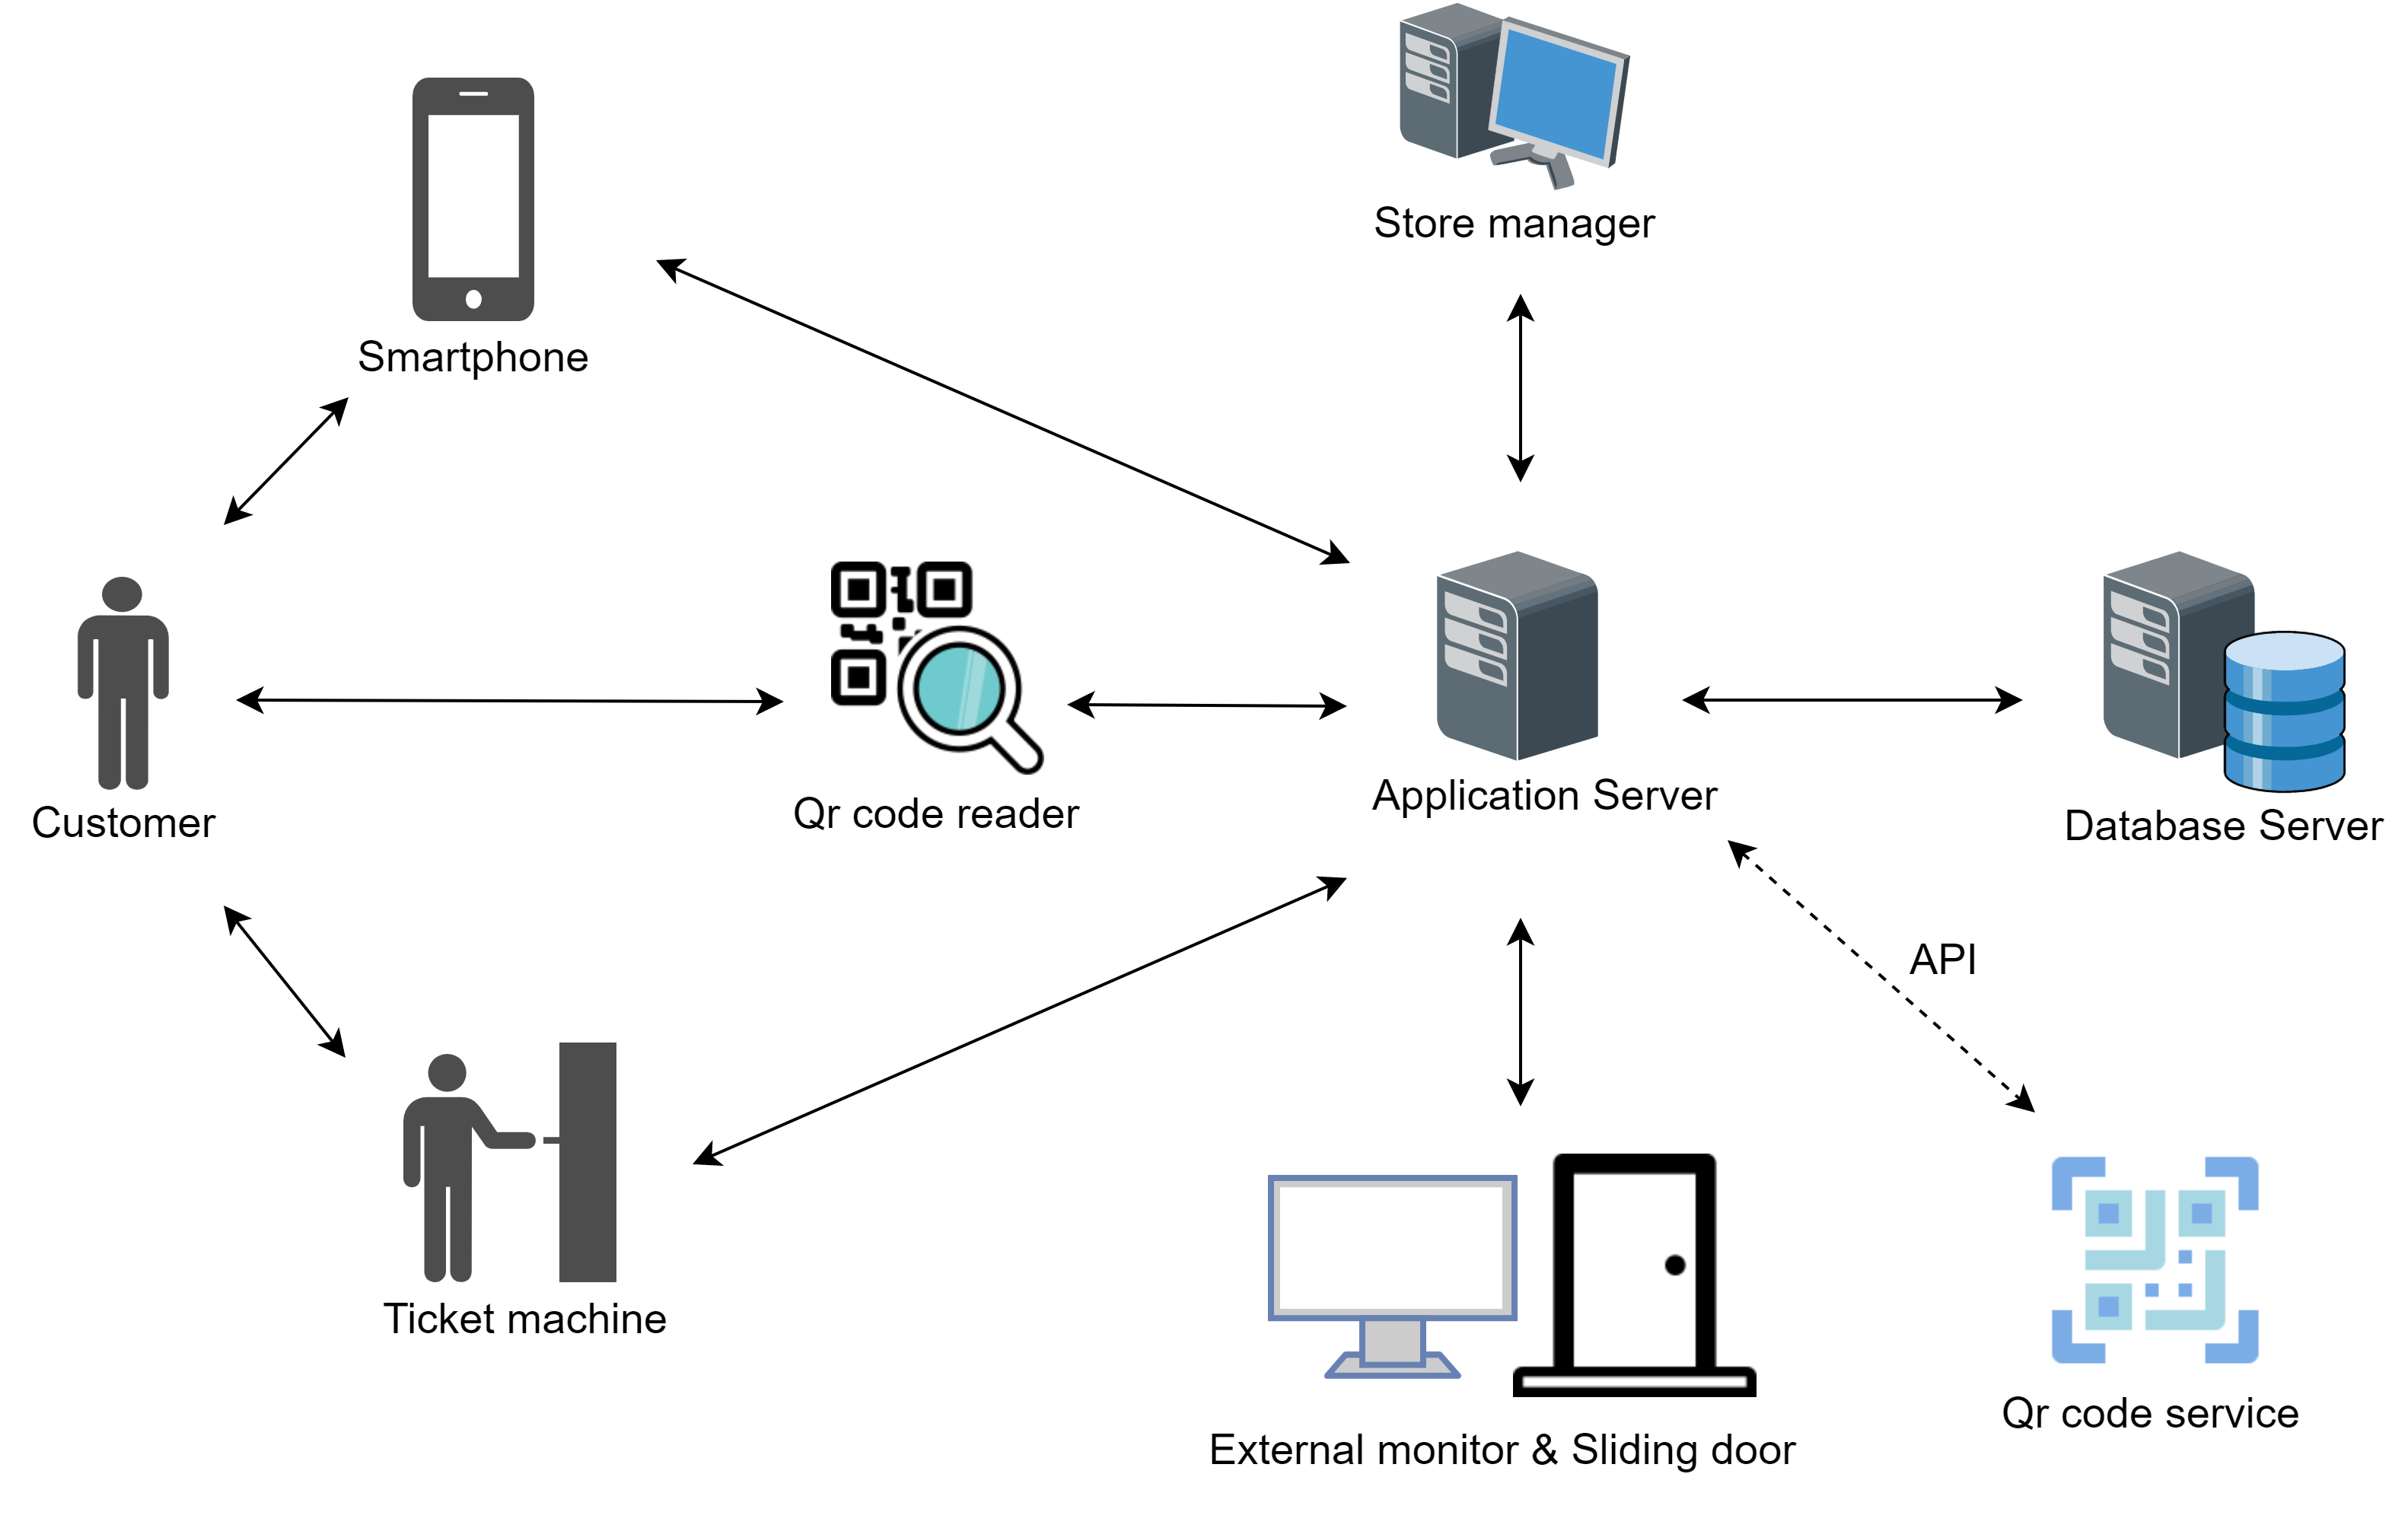
\includegraphics[scale=0.8]{HighLevelDiagram}
		\caption{CLup high Level architecture diagram}
	\end{figure}


\newpage
				

				

	\subsection{Component view}
	\textbf{} \newline
	\textbf{Component Diagram} \newline
	In the current section will be explained the interactions of the various components that the system contains. The component view diagram allows to better understand the flow in the \textbf{Application Server}, which is organized in multiple subsystems so that the different competence areas are properly divided with respect to the functionality they’re built for. A top-down approach has been used to define the properties and the functionalities of the various components of the system: to be more understandable, subsystems identify macro-area sections so that in a second moment they are specifically analyzed and explained.\\
The various components can communicate with each other through different interfaces. 
There are three components in the client side : the \textbf{customer} and the \textbf{store manager apps} and the \textbf{totem} where people take their physical ticket, which is connected to the application server too. The \textbf{Router} takes care to redirect to the proper subsystem or component the requests and responses that are generated during the lifetime of the system.\\
In the Application Server the \textbf{StoreHandler} and the \textbf{CustomerHandler} components are made so that they can handle the basic functions of the communication between the system and the store on one hand and between the system and the customer on the other one. General apps notifications and features that are not included in the ones that populate the queuing and book a visit subsystems rely here. They can both handle information requested by the users and retrieve the results they ask for, for example they can show what are the available stores in the neighborhood or retrieve current updated data from the stored statistics. In this way, if the system will handle and implement in the future some other small possible functions, these two components could be the ones that could handle the communications to guarantee to the store managers and the customers the best experience possible in the application.\newline\newline
What’s more, the application server is connected to:\\
	\begin{itemize}
		\item 	\textbf{QRcodeManager}: it cares about the generation/recognition of the tickets.
		
		\item 	\textbf{StoreSlidingDoors}: it allows to open the doors of the shop.
		
		\item 	\textbf{GoogleMapsService}: computes the time and the distance between the costumer and the store.	
	
	\end{itemize}
	
	\textbf{} \newline
For the sake of completeness it has been shown also the \textbf{DBMS service}, but the main focus is made towards the Application Server, which is the core of the application’s logic. \newline\newline
In the following paragraphs the various subsystems will be briefly explained.\\


	\newpage \textbf{}\\\\
\bigskip \bigskip \bigskip
	\begin{figure}[H]
			\centering
			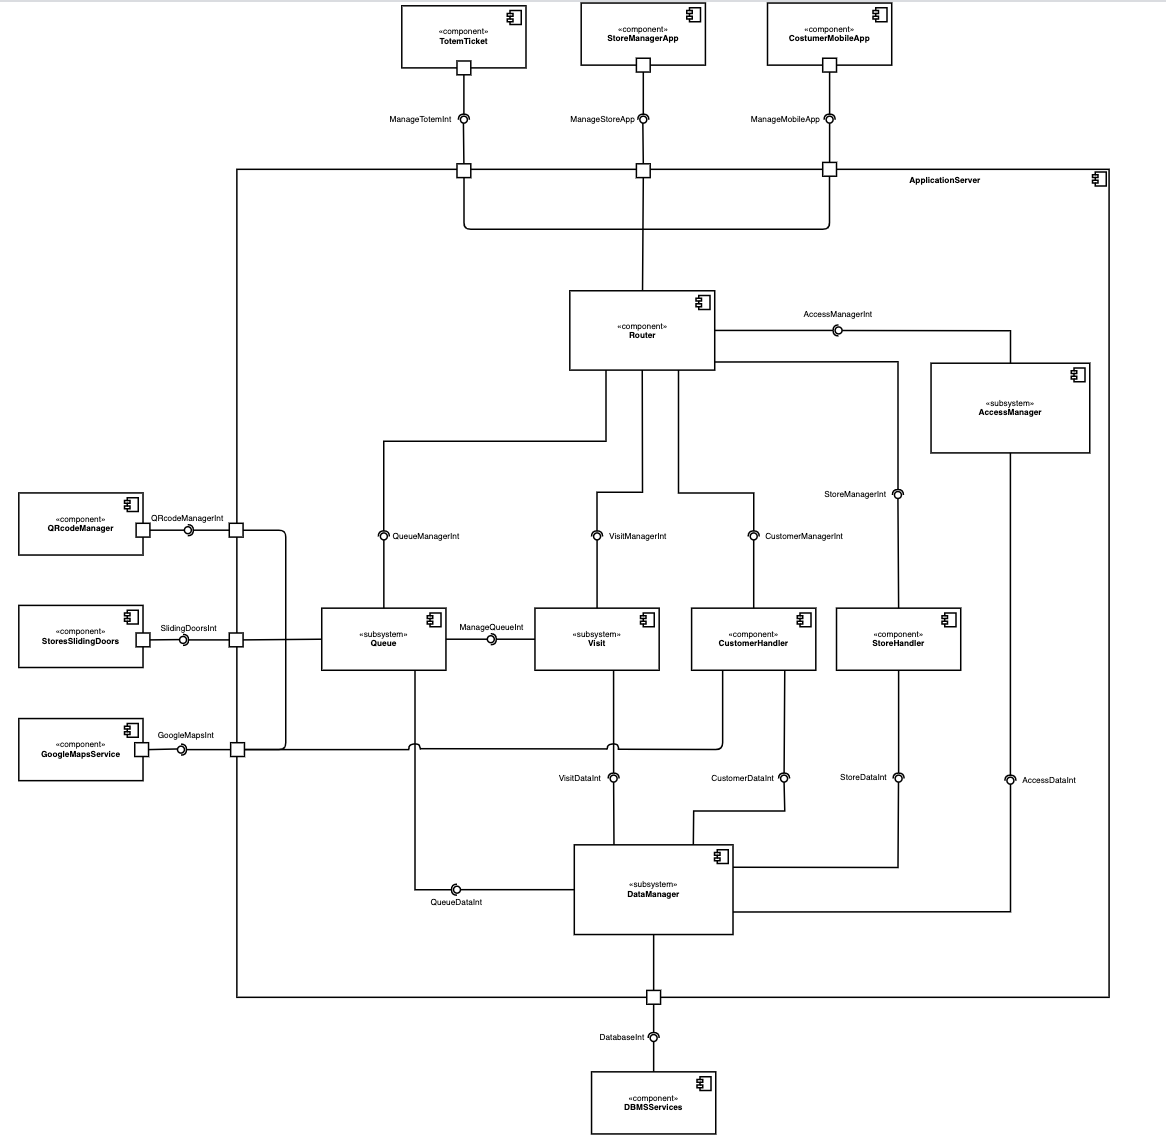
\includegraphics[scale=0.3]{ComponentView/ComponentViewDiagram.png}
			\caption{General Component Diagram}
			\label{fig:ComponentDiagram}
		\end{figure}
		\bigskip\bigskip
	\newpage
	\noindent
	\textbf{Access Manager subsystem} \newline
	The access manager cares about the sign up and the login of the users, both the customers and the store managers. The access is handled differently for the two entities (\textbf{AccessStoreManager} and \textbf{AccessCustomer}), that have to provide different kind of information (the signing up and the authentication is different if the user is a store, because the system needs to accurately verify through some given documents the validity and the existence of the shop, while the sign up of a customer is more immediate because an existent valid email and a password would be sufficient), and the access to the data manager can be made with different purposes: with the sign up data are stored in the database, so that users are registered to the system, while with the login the validity of the inserted data (username and password) are checked with the ones that are already stored in the DB. 
	\bigskip
	\begin{figure}[H]
			\centering
			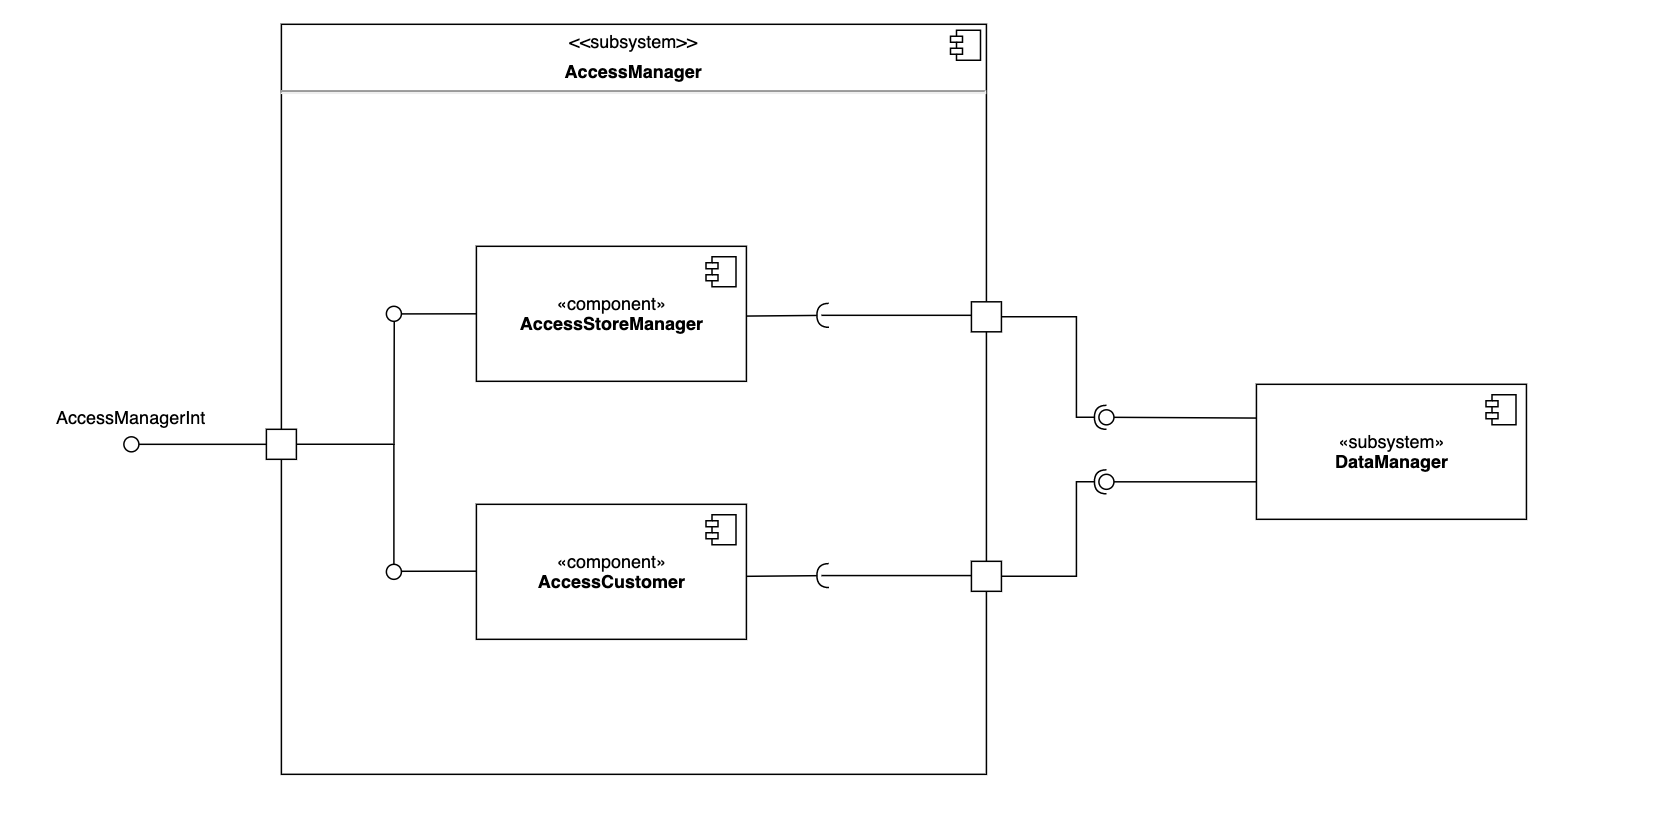
\includegraphics[scale=0.6]{ComponentView/AccessManagerComponent.png}
			\caption{AccessManager subsystem component diagram}
			\label{fig:AccessManagerDiagram}
		\end{figure}
		\bigskip\bigskip
	\newpage
	\noindent
	\textbf{Queue subsystem} \newline
	The Queue subsystem is the part of the system devoted to handle the people queueing to the store.
	Its responsabilities concern updating and managing the queue of people to a certain store, provide notification to users when they need to start approaching the store and handle the creation/recognition of Qr code tickets interfacing with an external module.
	The Queue subsystem is composed of three main components:
	
	\begin{itemize}
		\item 	\textbf{QueueHandler} is devoted to handling the queue logic beside of the application. It is responsible for putting users in the queue as well as removing them when their turn has come. It interacts with the Data Manager to store data about the queue and with the Sliding door interface to lock/unlock the door accordingly to Qr code scannings.
		
		\item 	\textbf{NotificationService} takes care of notifing CLup users when they need to reach the store. It interfaces with GoogleMapsAPI in order to estimate the time a user needs to reach the store given his position and transport mean.
		
		\item 	\textbf{Ticket Manager} is responsible for interfacing with the external software component \textit{QrcodeManager} in order to create, assign and recognize Qr codes.
		
	
	\end{itemize}

	\bigskip
	\begin{figure}[H]
			\centering
			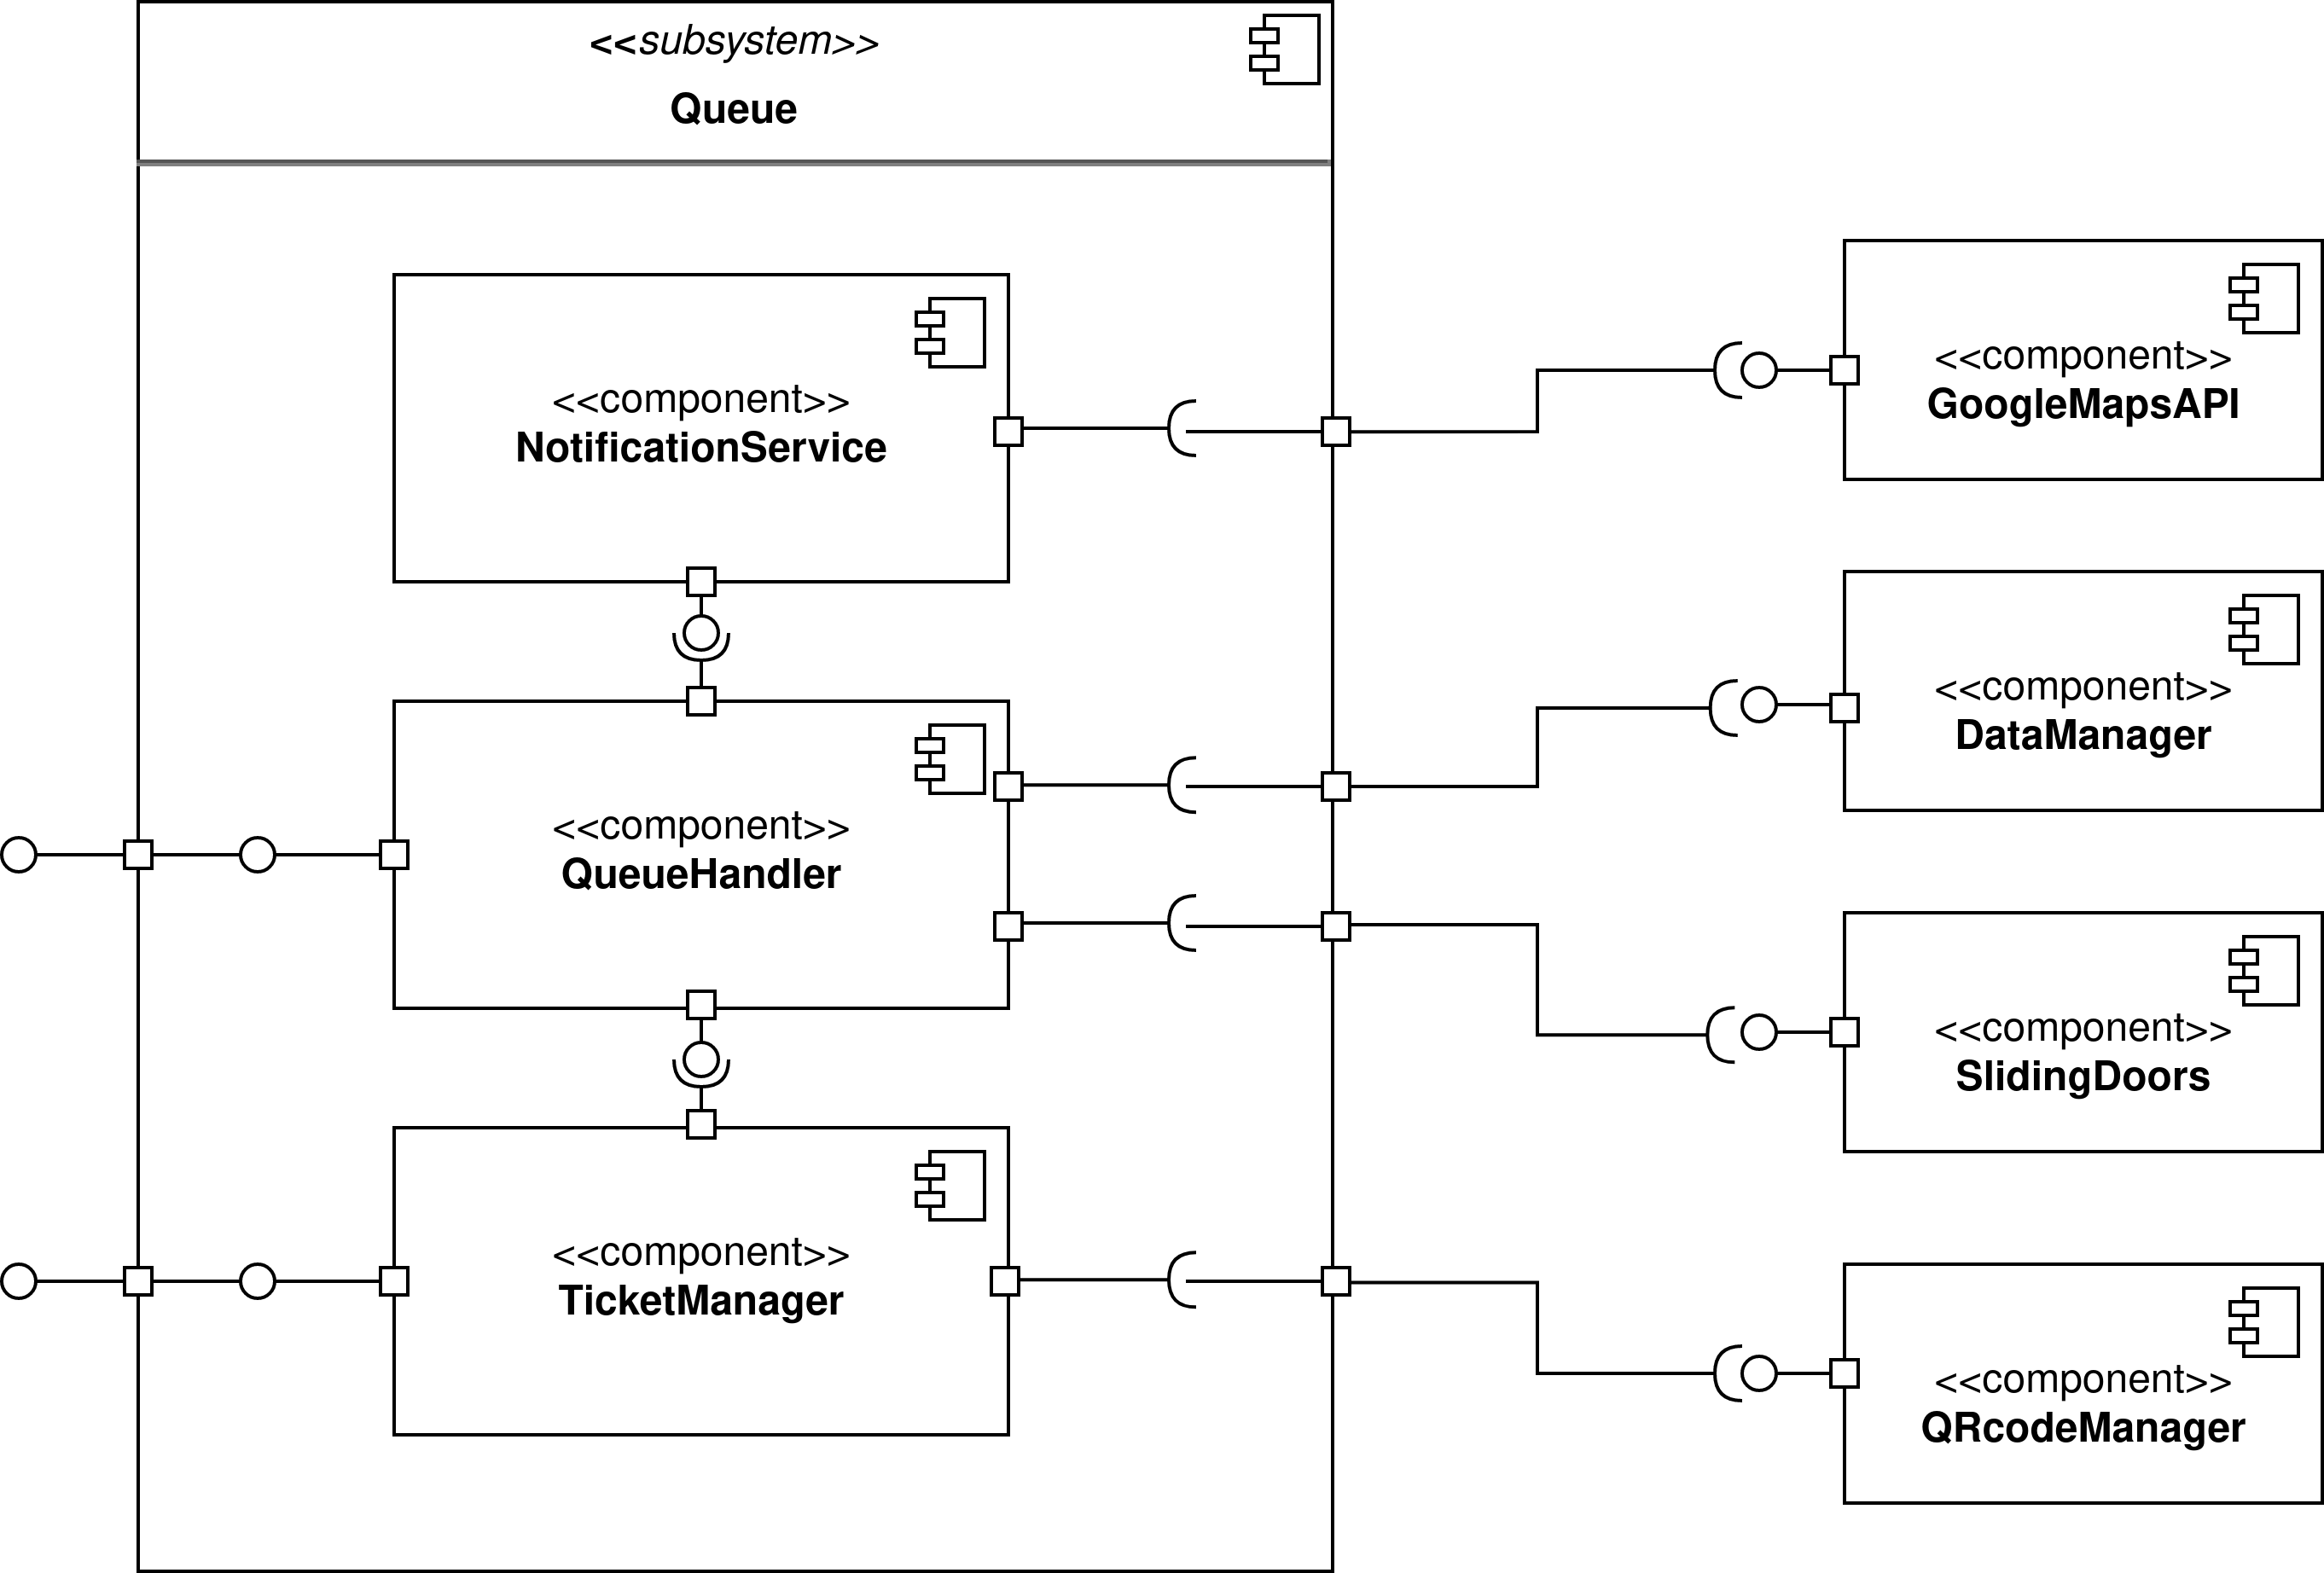
\includegraphics[scale=0.9]{ComponentView/queueComponent.png}
			\caption{Queue subsystem component diagram}
			\label{fig:Queuediagram}
		\end{figure}
		\bigskip\bigskip
		
	\newpage
	\noindent
	\textbf{Visit subsystem}
	\medskip \newline
	The visit subsystem aims to handle everything that is related to booking visits. It is composed by 4 components as the reader can see in the picture below. 
	\bigskip
	
	\begin{figure}[H]
		\centering
		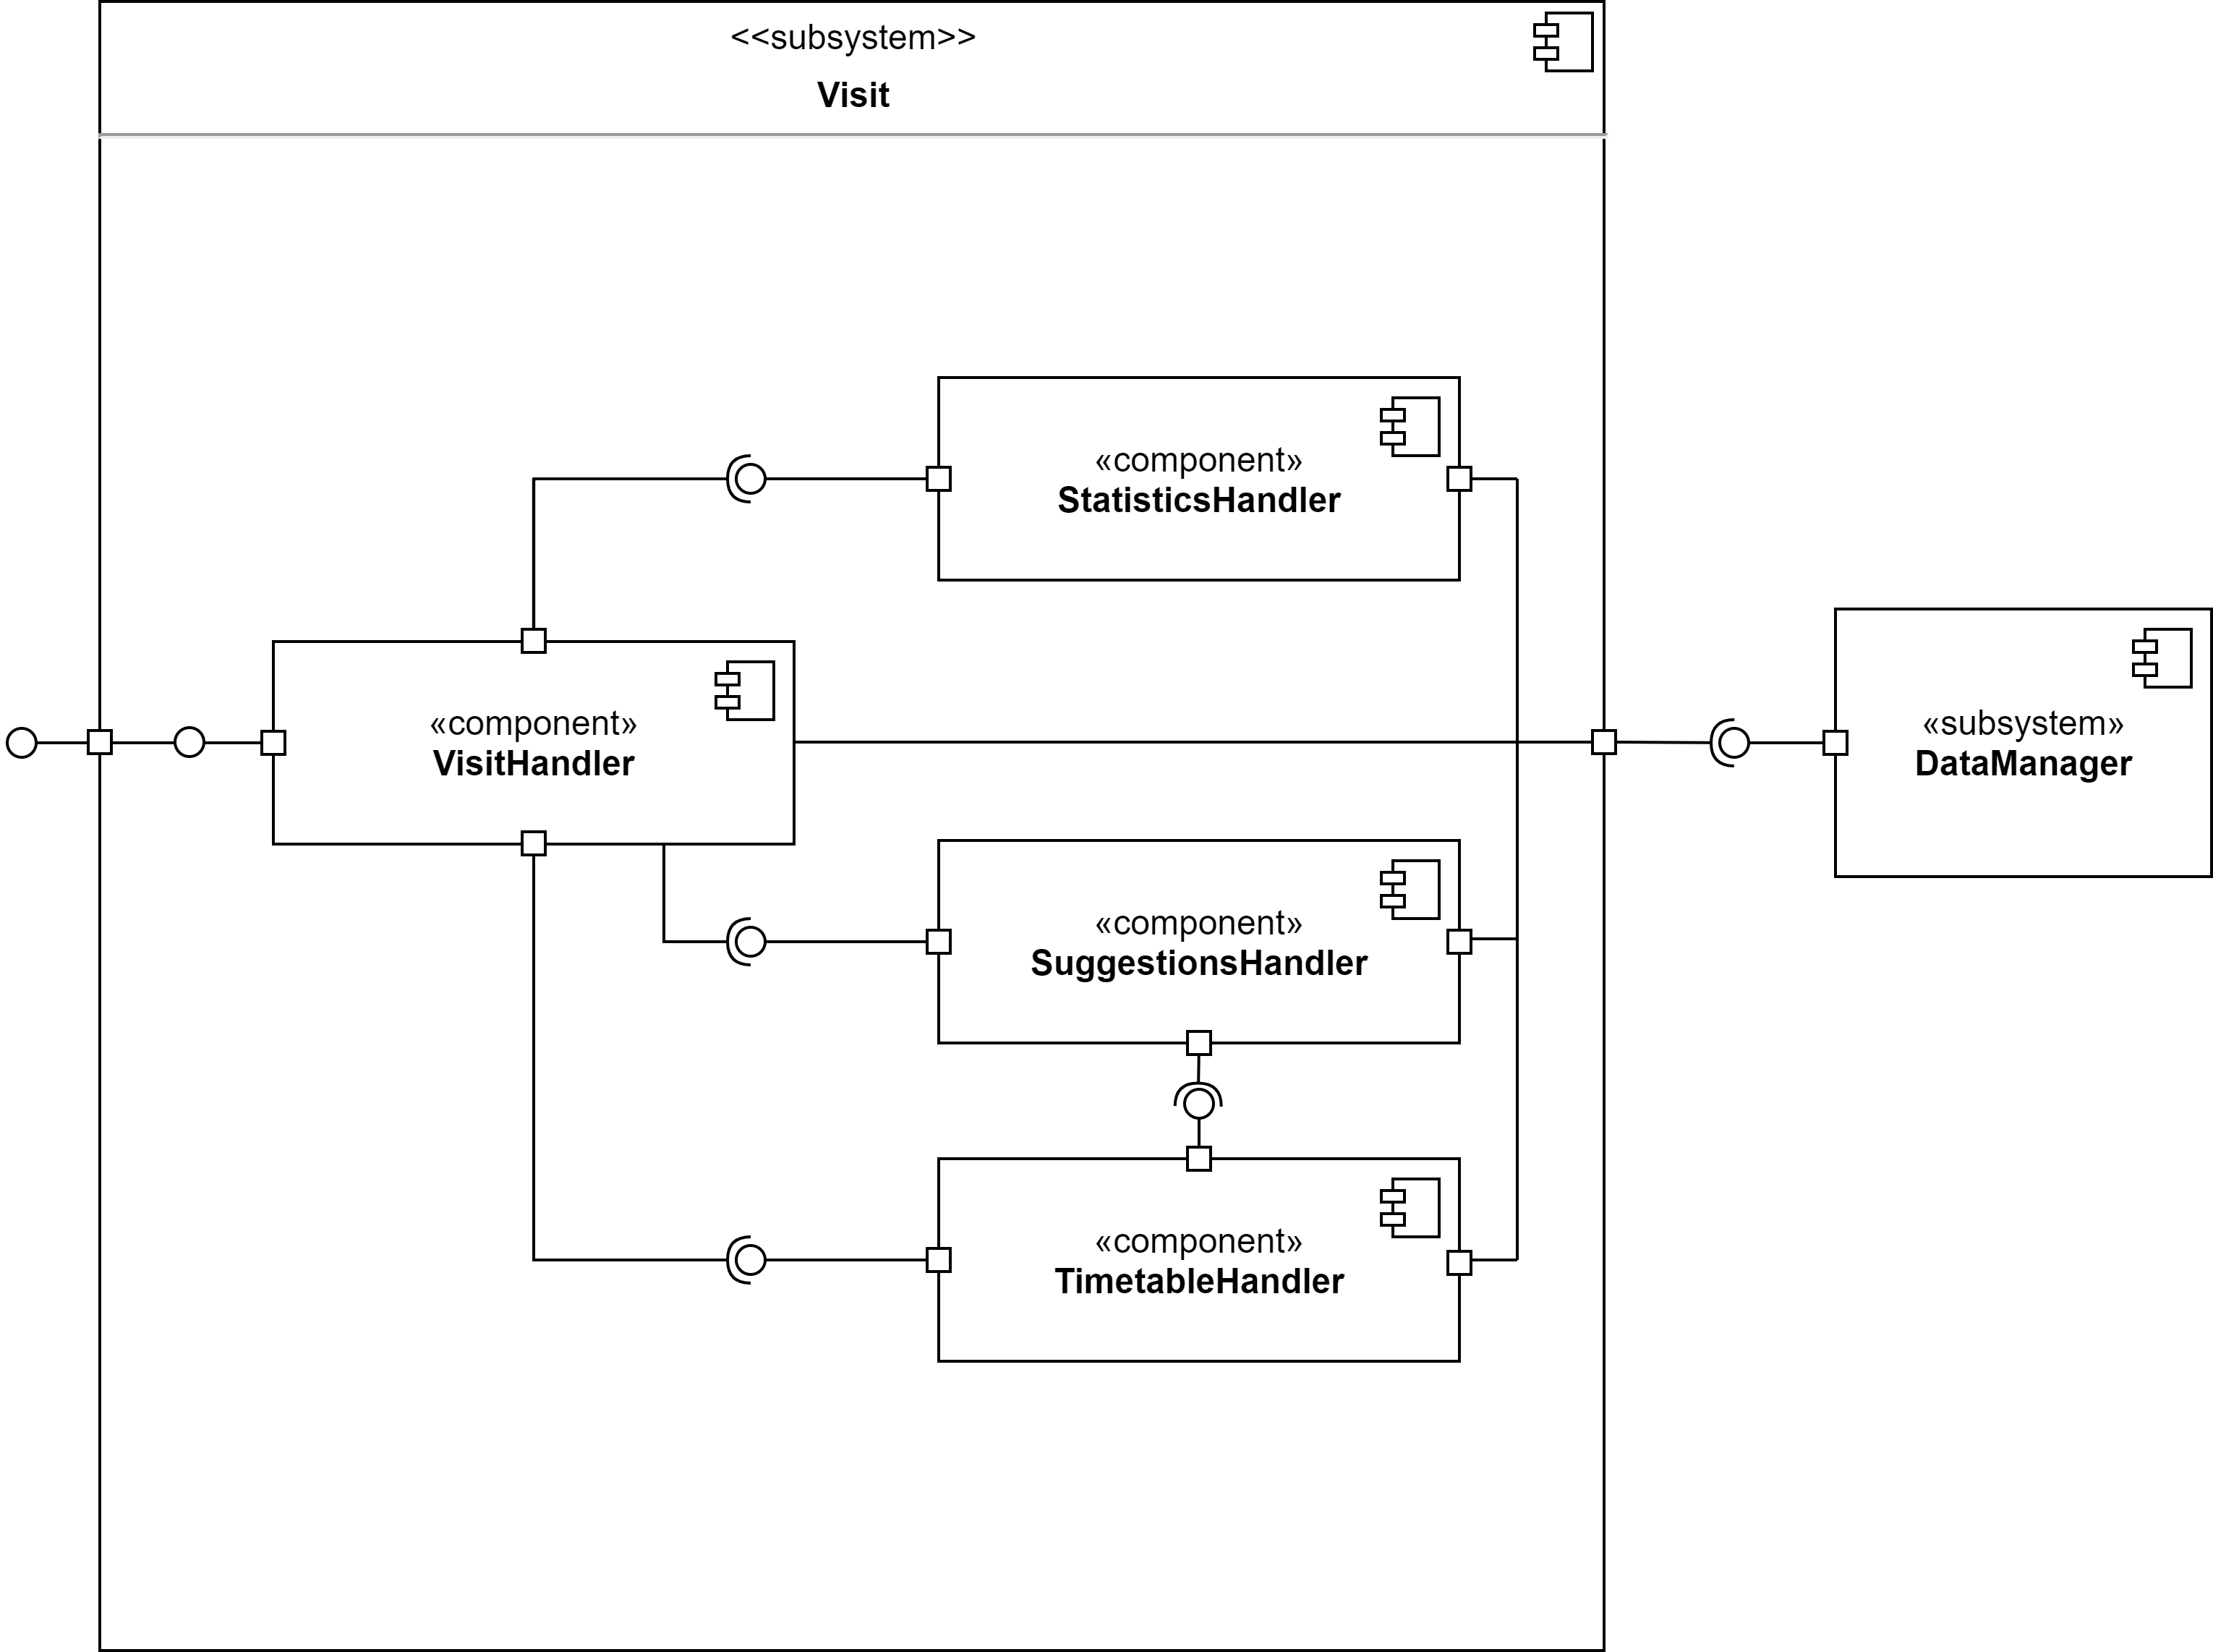
\includegraphics[scale=0.73]{ComponentView/VisitComponent}
		\caption{Visit subsystem}
		\label{fig:visitSubsystem}
	\end{figure}
	\bigskip
	\begin{itemize}
		\item \textbf{VisitHandler} fulfill the main booking visits tasks and works as an "orchestrator" of this subsystem.
		Firstly it handles the requests that comes from outside this subsystem. To performs its tasks VisitHandler combines its "general" capabilities with the more specialized functionalities offered by the other components;
		\item \textbf{StatisticHandler} collects user statistics and provide them to VisitHandler. There's a strong connection with the DataManager component which is a link to the database, where the statistic are stored;
		\item \textbf{SuggestionsHandler} computes the suggestions showed to the user during the booking visit phase;
		\item \textbf{TimetableHandler} take care of the visits timetable. For example it is able to return the available visits time-slot.
	\end{itemize}
	

	
		\newpage
		\noindent		
		\textbf{Data Manager subsystem} \newline
		\noindent
		The purpose of the Data Manager subsystem is creating a common interface, shared with ther whole system, to access data stored in the database. \newline
		Instead of using directly the DBMS API, each component that needs to manipulate data that are stored in the DB is forced to use one of the two components that make the subsystem. \newline
		The reason behind this decision is to \textbf{decouple} our system from the DBMS: a change in the DBMS API or switching DBMS vendor will affect only our Data Manager subsystem instead of the whole application. \newline
		In particular:
		
		\begin{itemize}
		
			\item \textbf{DataRetriever} is devoted to data fetching
			\item \textbf{DataStorer} is responsible for storing data in the DB
		\end{itemize}
		
			\begin{figure}[H]
			\centering
			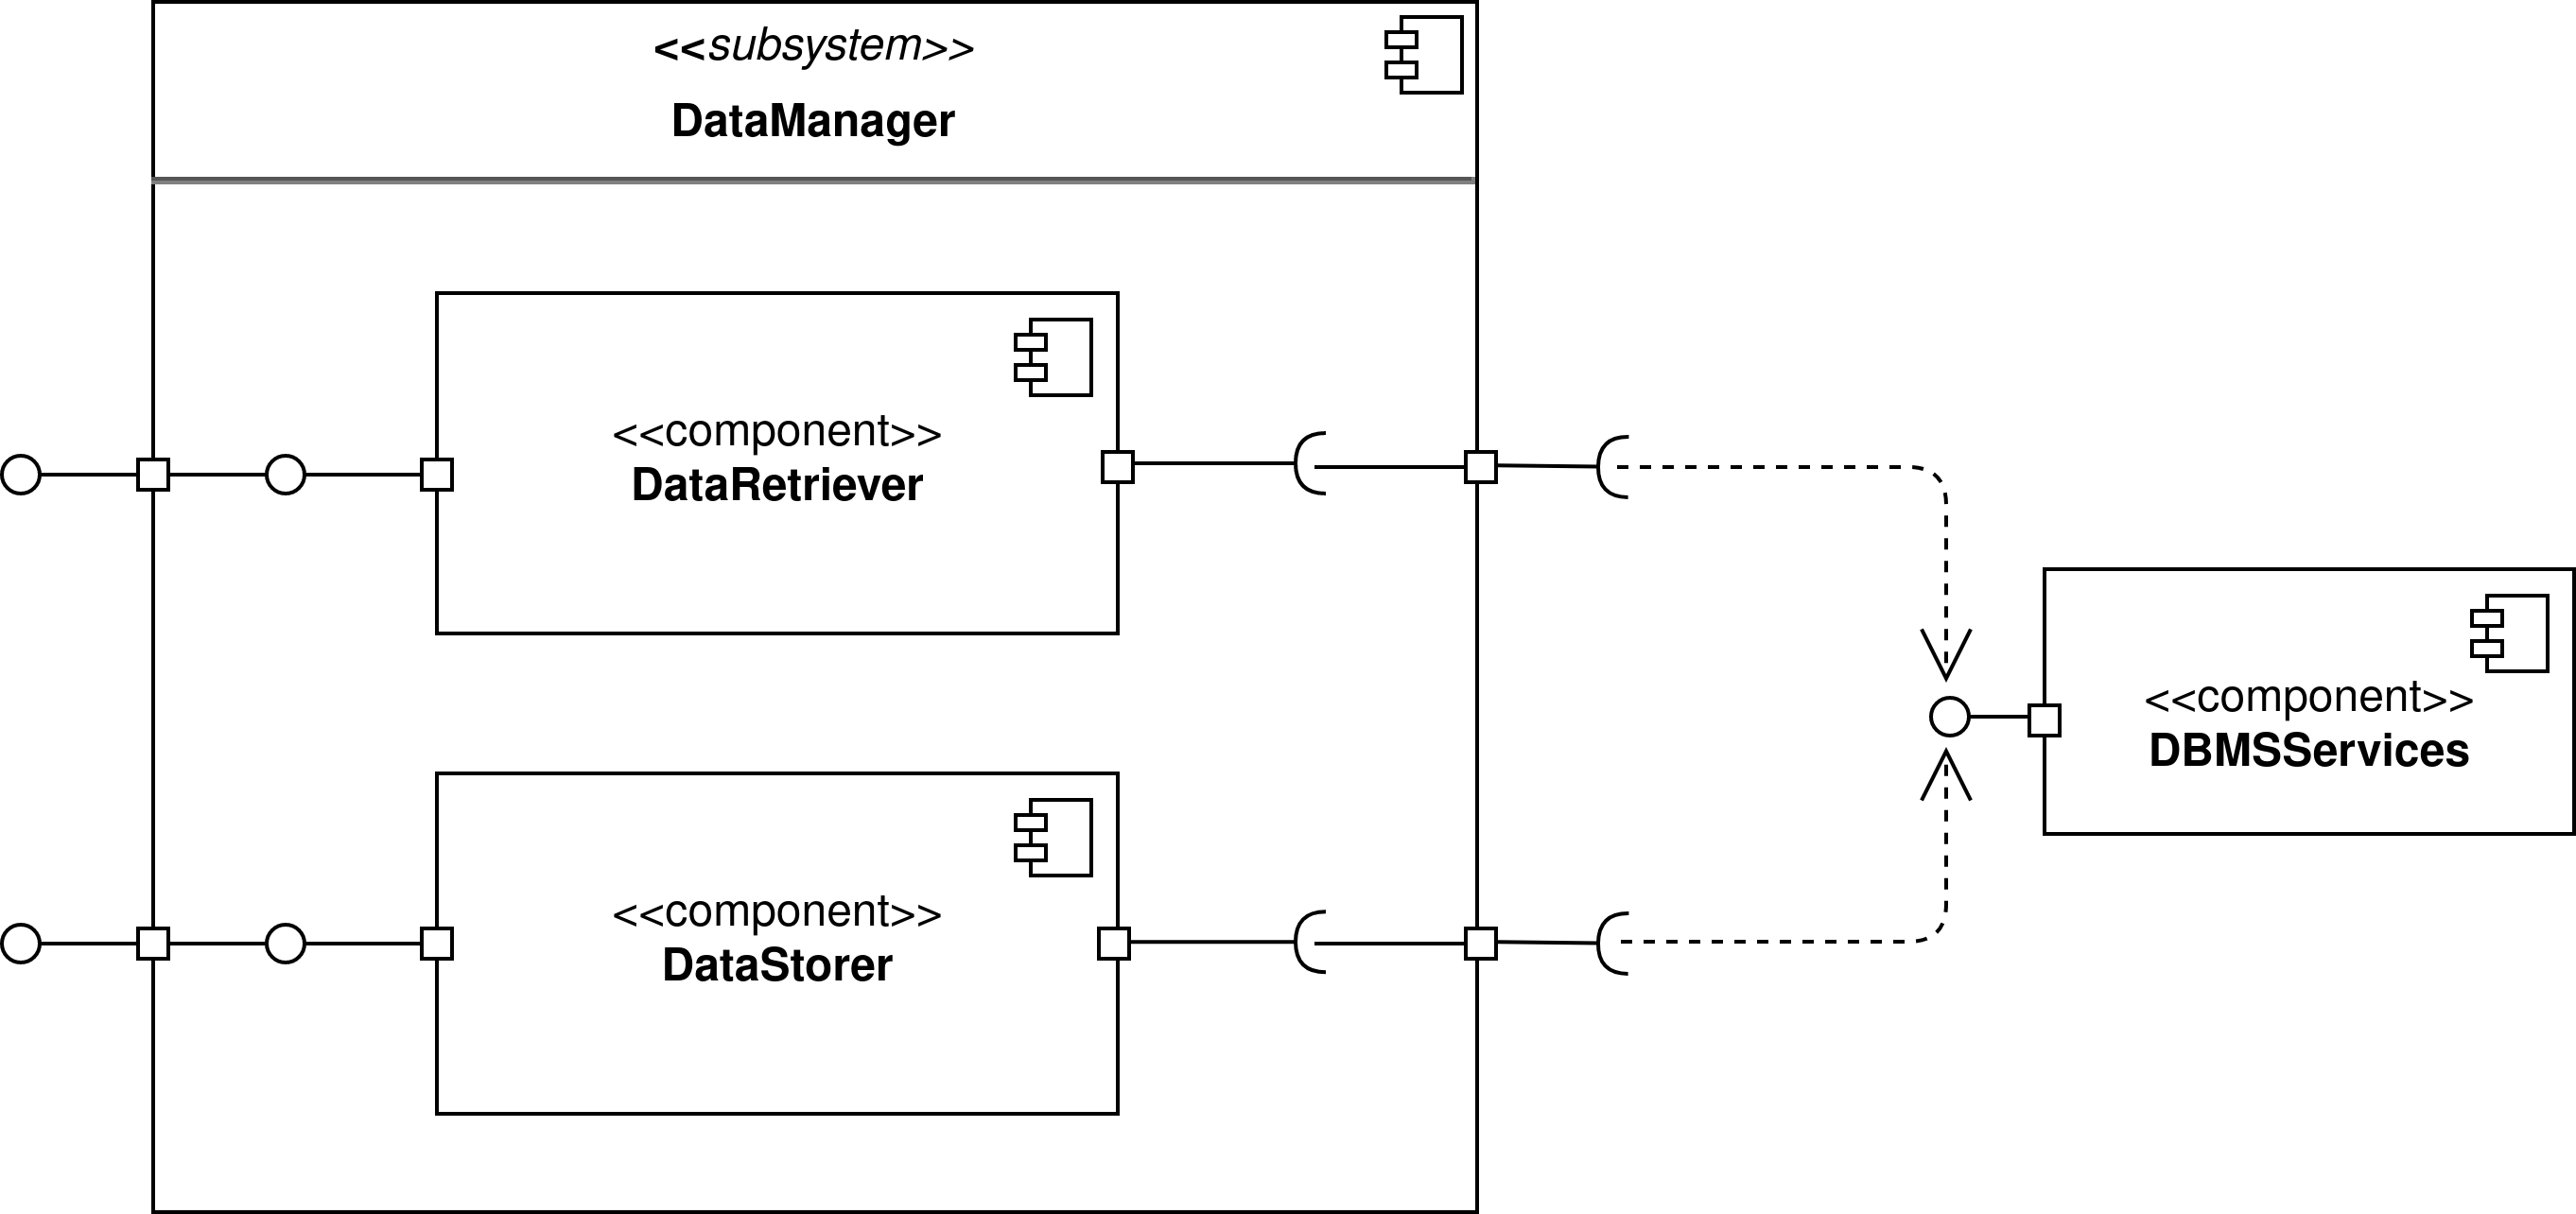
\includegraphics[scale=0.9]{ComponentView/DataManagerComponent.png}
			\caption{Data Manager subsystem component diagram}
			\label{fig:DataManagerDiagram}
		\end{figure}
		
	\bigskip
	\newpage
	\noindent
	\subsubsection{UML - Model Class Diagram}
	Moreover, the following diagram shows a general UML representation of the system's Model. \newline
	Each component that interacts with the Model is supposed to interface with the DataManager component and invoke the methods for retrieving/storing data. \newline
	\bigskip \bigskip
	\begin{figure}[H]
			\centering
			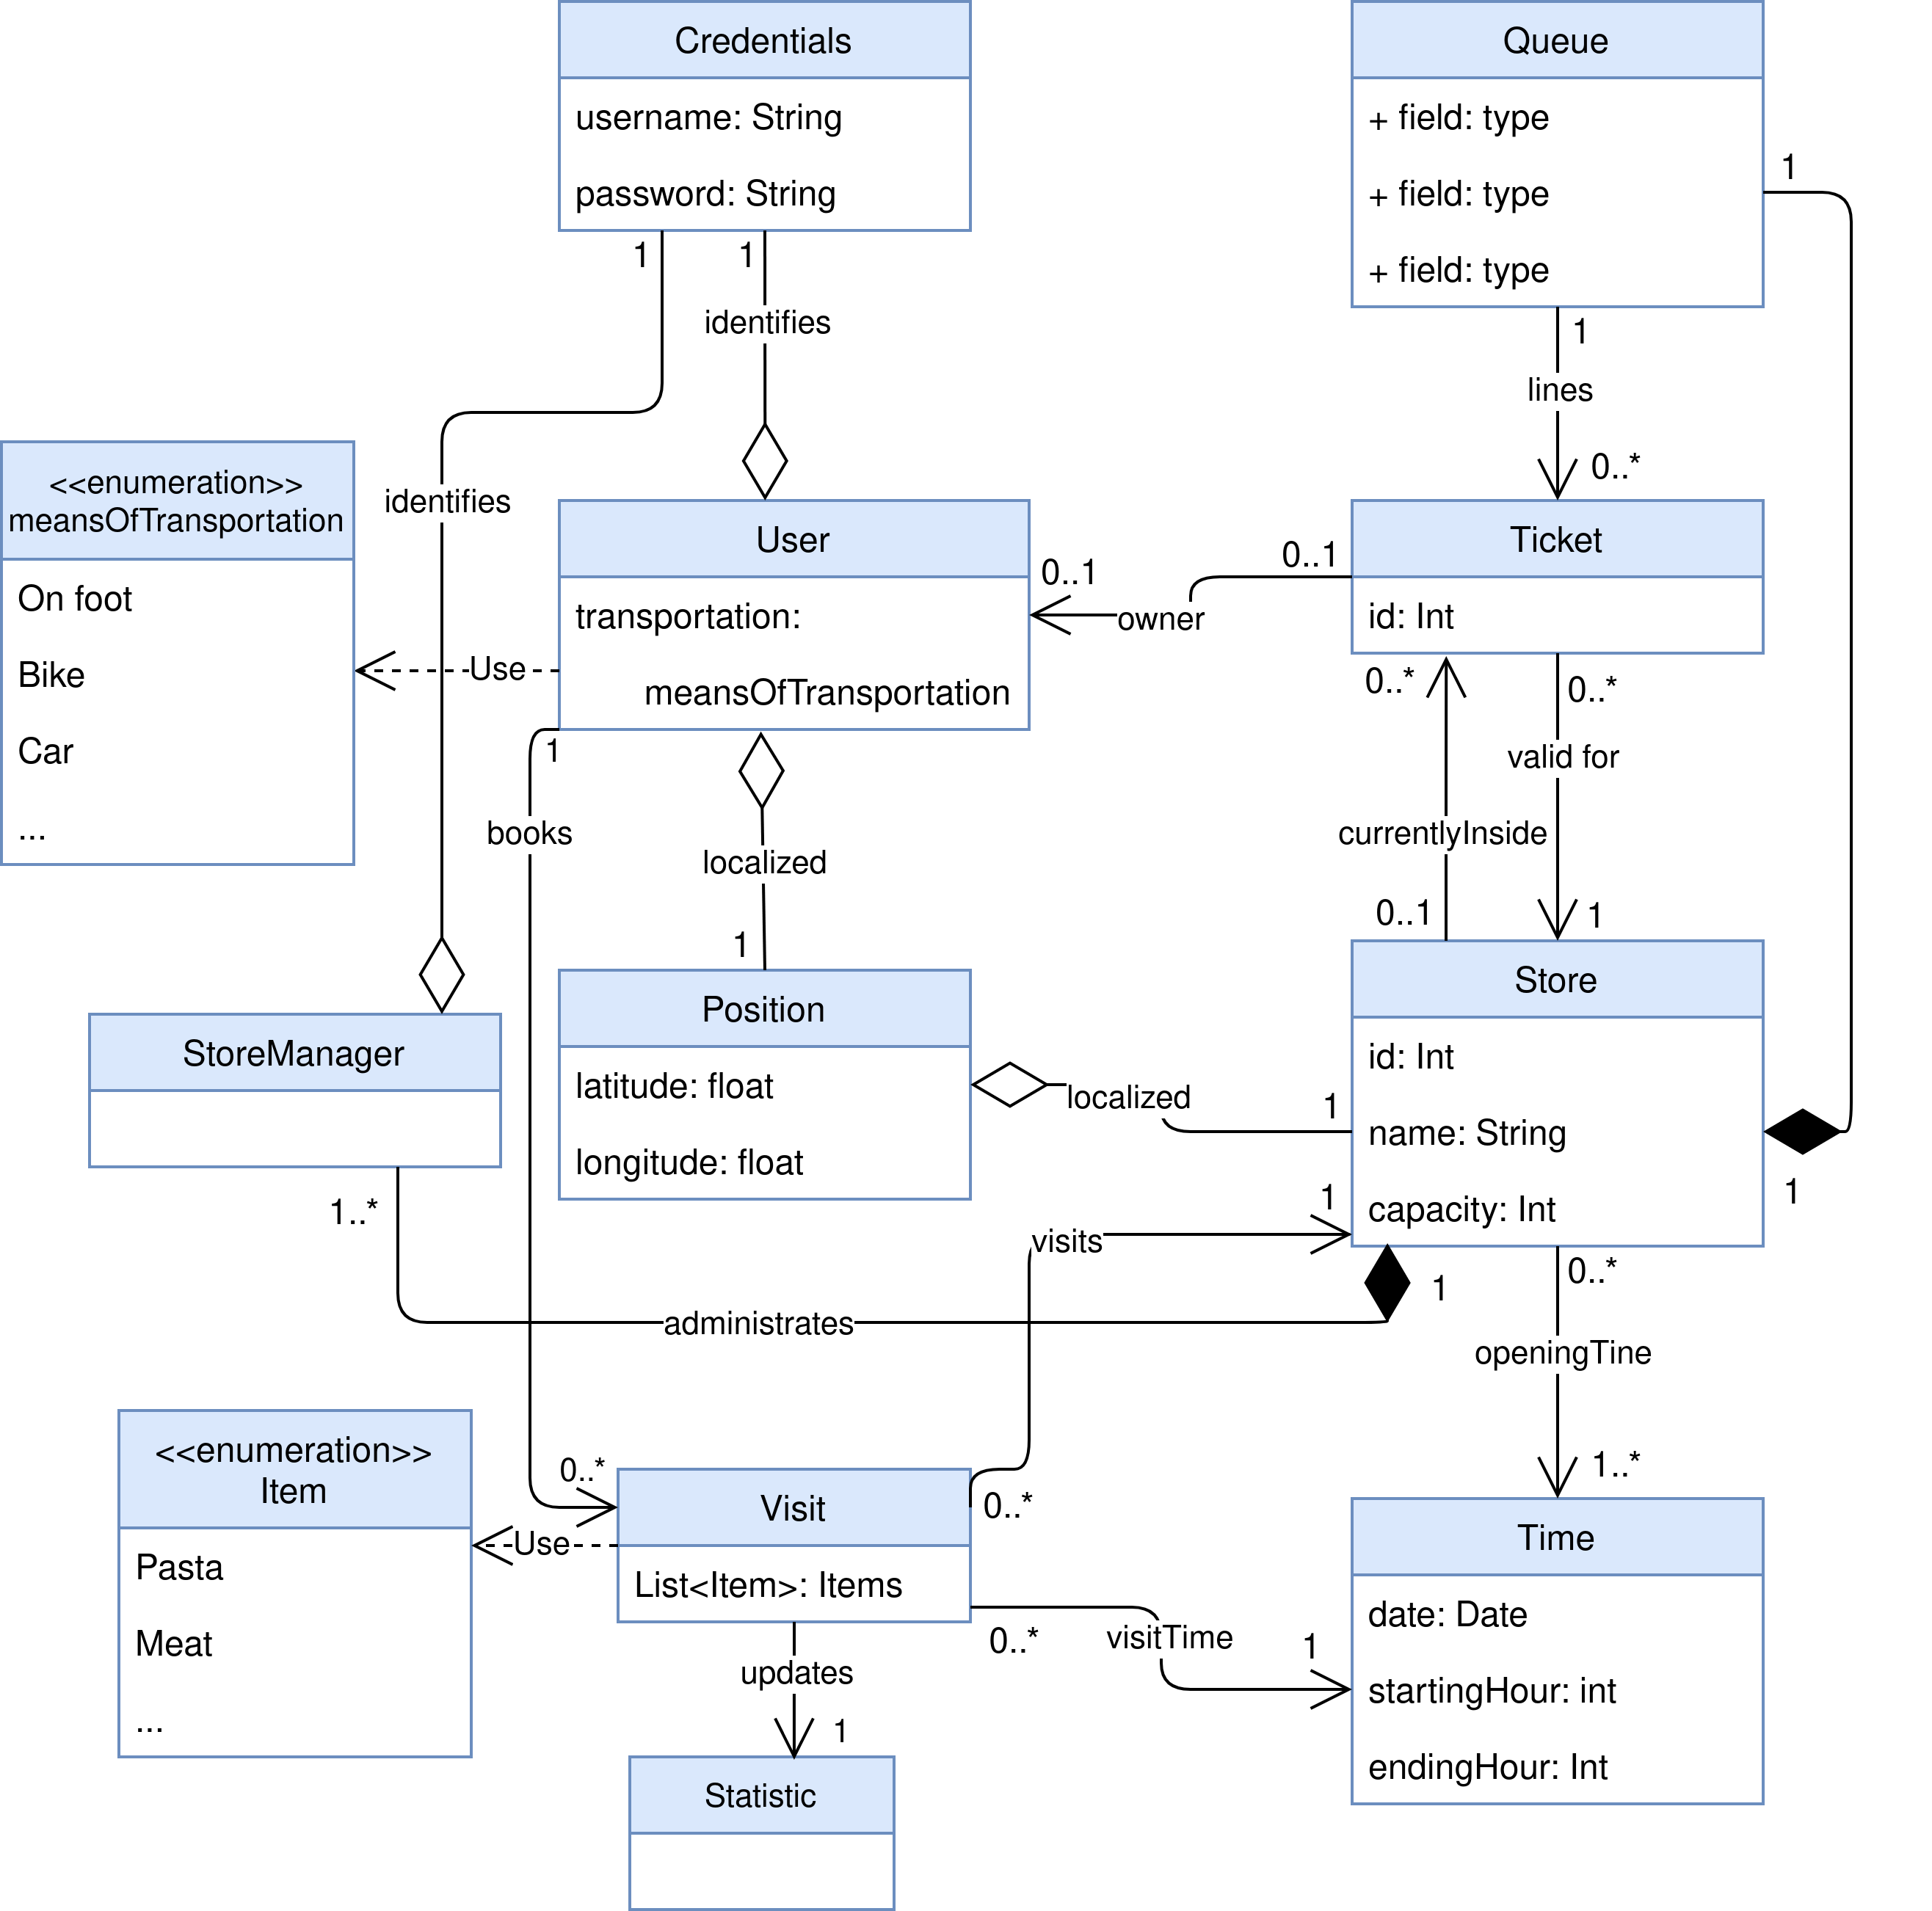
\includegraphics[scale=0.93]{ComponentView/umlDD.png}
			\caption{Model UML diagram}
			\label{fig:ModelUML}
		\end{figure}
	
		
	
	
	
	\newpage
	\subsection{Deployment view}
	The figure below shows the distribution of the CLup components among the hardware ones. Some details are omitted, like the external interfaces, to maintain the focus on the main components of each architecture tier. 
	\newline
	\begin{figure}[H]
		\centering
		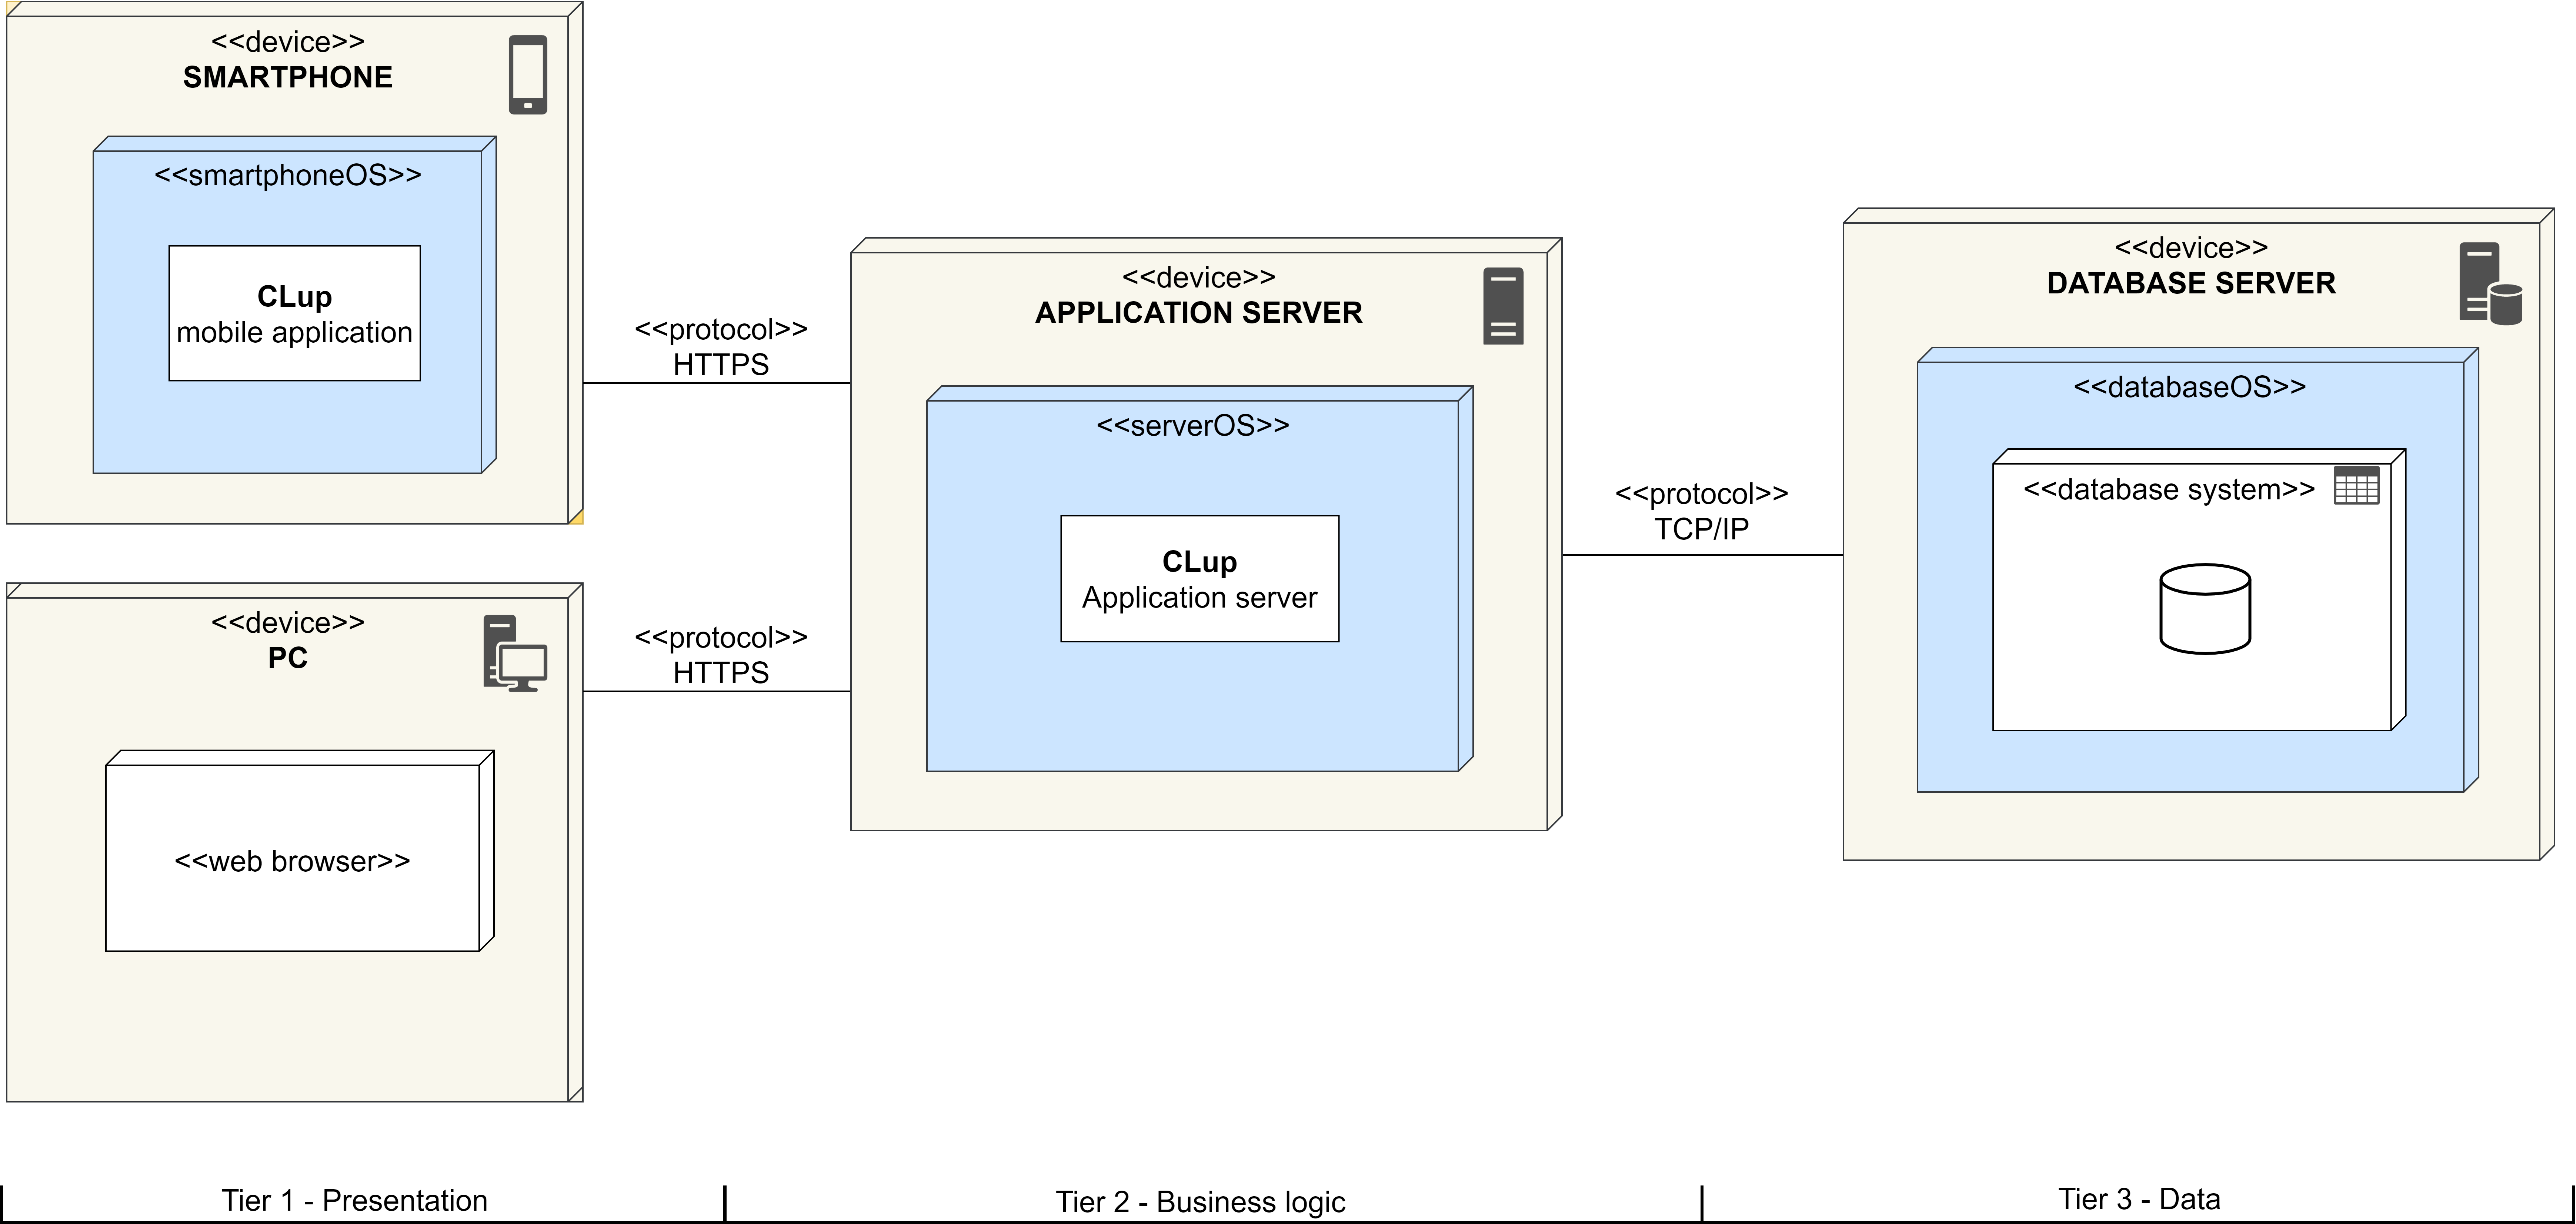
\includegraphics[scale=0.38]{deployment}
		\caption{CLup deployment view}
		\label{fig:deployment}
	\end{figure}


	\bigskip
	\noindent	
	The presentation tier contains the devices by which costumers and store managers can interact with the system. Costumer can use their own smartphones where they have to install the CLup mobile application. There are no restrictions about the operating system of the device, the app must be developed both for Android and IOS, for being compatible with the almost totality of the smartphone. 
	\\On the other side, store managers can interact with CLup with any personal computer by means of the CLup web application, therefore they don't have to install anything but a web browser.
	The reader should notice the communication protocol between the personal devices and the Application Server: HTTPS.
	\newline\newline
	The intermediate tier contains the core of the CLup software system. Firstly, as the reader can see in the component diagram, the Application Server performs all the tasks related to the business logic. 
	Secondly, this tier has the task of manage all the requests that come from the users devices. 
	In this case the technology involving the server device and its operating system are left to the developers.
	\newline\newline
	Finally, in the third tier, Database Server, is located the data management. Whenever the Application Server has to store or retrieve data it has to exploit the components of this tier. As in the second tier, the choice of the device of this server and its operating system is left to the developers. The only recommendation is about the nature of the database. A relational one must be preferred for a better general organization of the CLup data. 
	
	\newpage
	
	\subsection{Component interfaces}
	
	The following diagram describes the main interfaces of the system. \newline
	They are not necessarily supposed to be developed as they are but their goal is to give an overview of what type of methods the interfaces are going to need. \newline
	Some minor interfaces were omitted while the \textit{RouterInterface} and \textit{DataManagerInterface} are not described as they are directly correlated to the other interfaces and can be easily derived. \newline
	The interfaces below represent the API of subsystems of components as shown in Figure \ref{fig:ComponentDiagram}. Each method will then be provided by one specific component that belongs to such subsystem.\newline
	\bigskip 
	\begin{figure}[H]
		\centering
		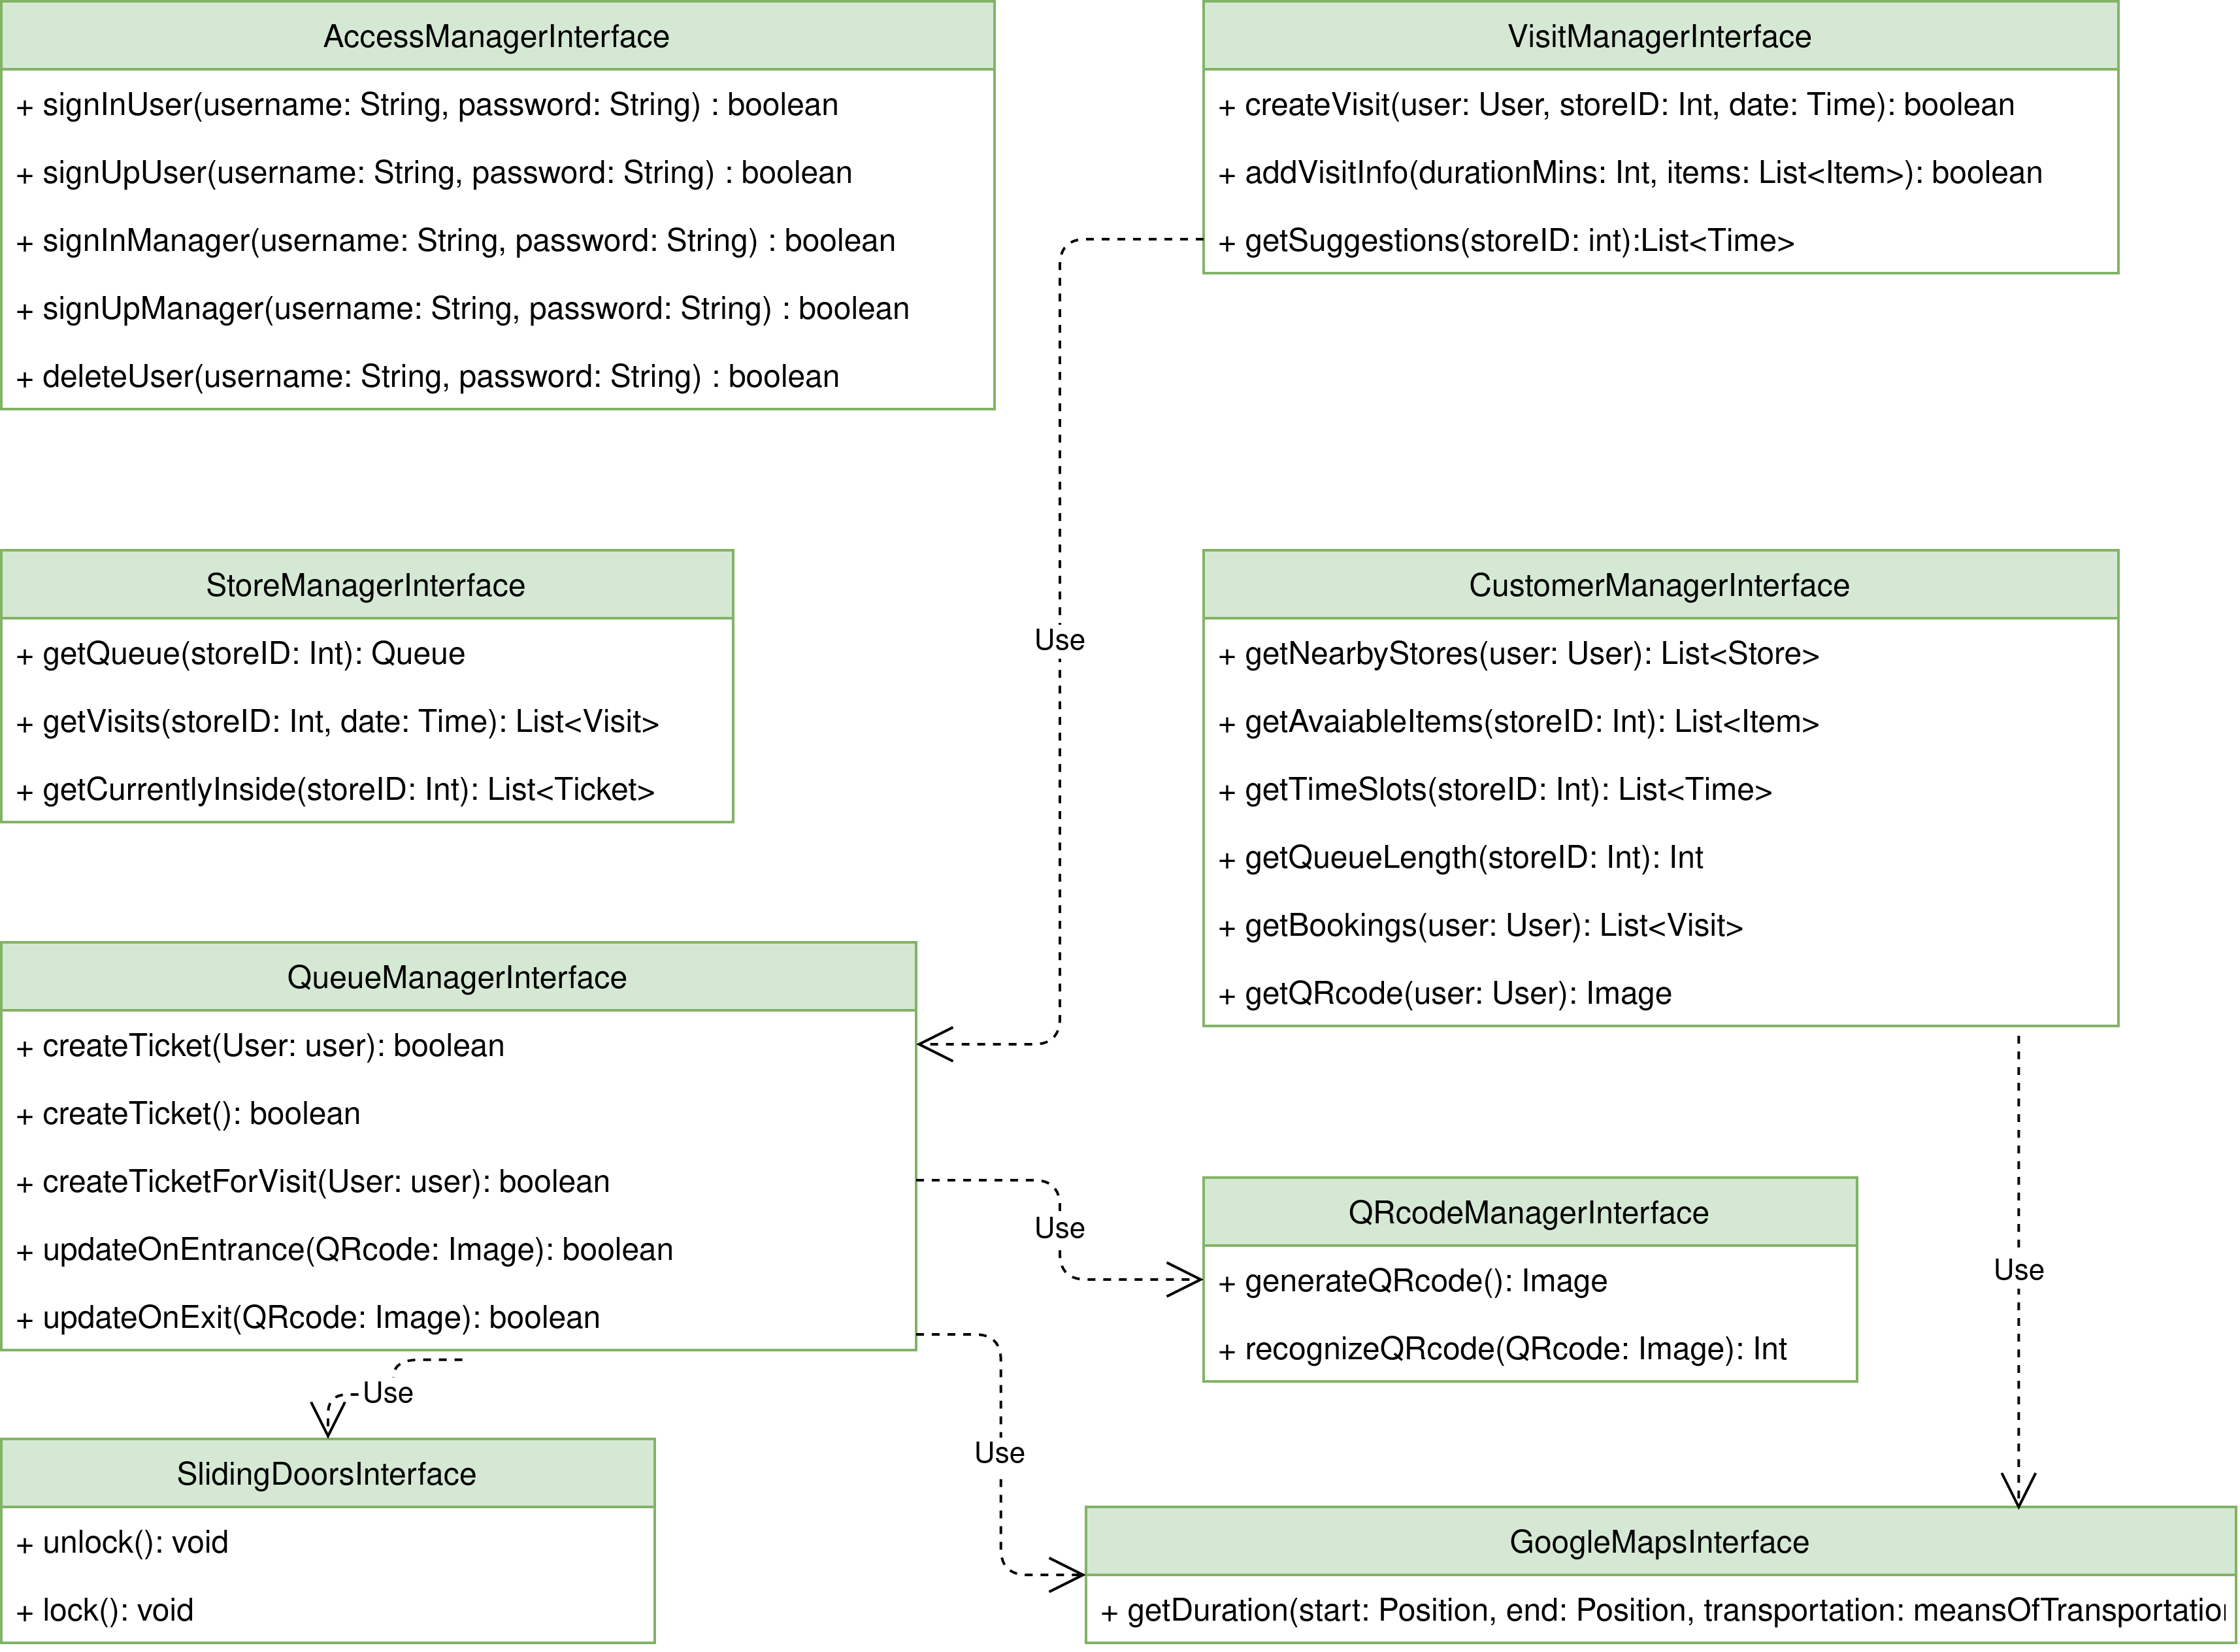
\includegraphics[scale=0.7]{ComponentView/componentInterfaces.png}
		\caption{Component interfaces}
		\label{fig:componentInterfaces}
	\end{figure}
	
	
	\newpage
	
	
	\subsection{Runtime View}
	The sequence diagrams presented below show the behavior of the system, in terms of components interaction. The diagrams are focused on the back-end computations, the interaction between the mobile application and the application server is not considered.
	\newline
	\newline
	\noindent
	\textbf{Line-up}
	\newline \newline
	The first sequence diagram takes into account the remote line-up of a costumer.
	After the costumer chooses the store and communicates the intention of line-up, the system starts the line-up procedure. QueueHandler, according to the data stored in the database, computes the feasibility of the line-up. In the case it is possible, TicketHandler and QRcodeManager generate the QRcodeTicket that is sent to the costumer.
	\bigskip
	\bigskip
	
	\begin{figure}[H]
		\centering
		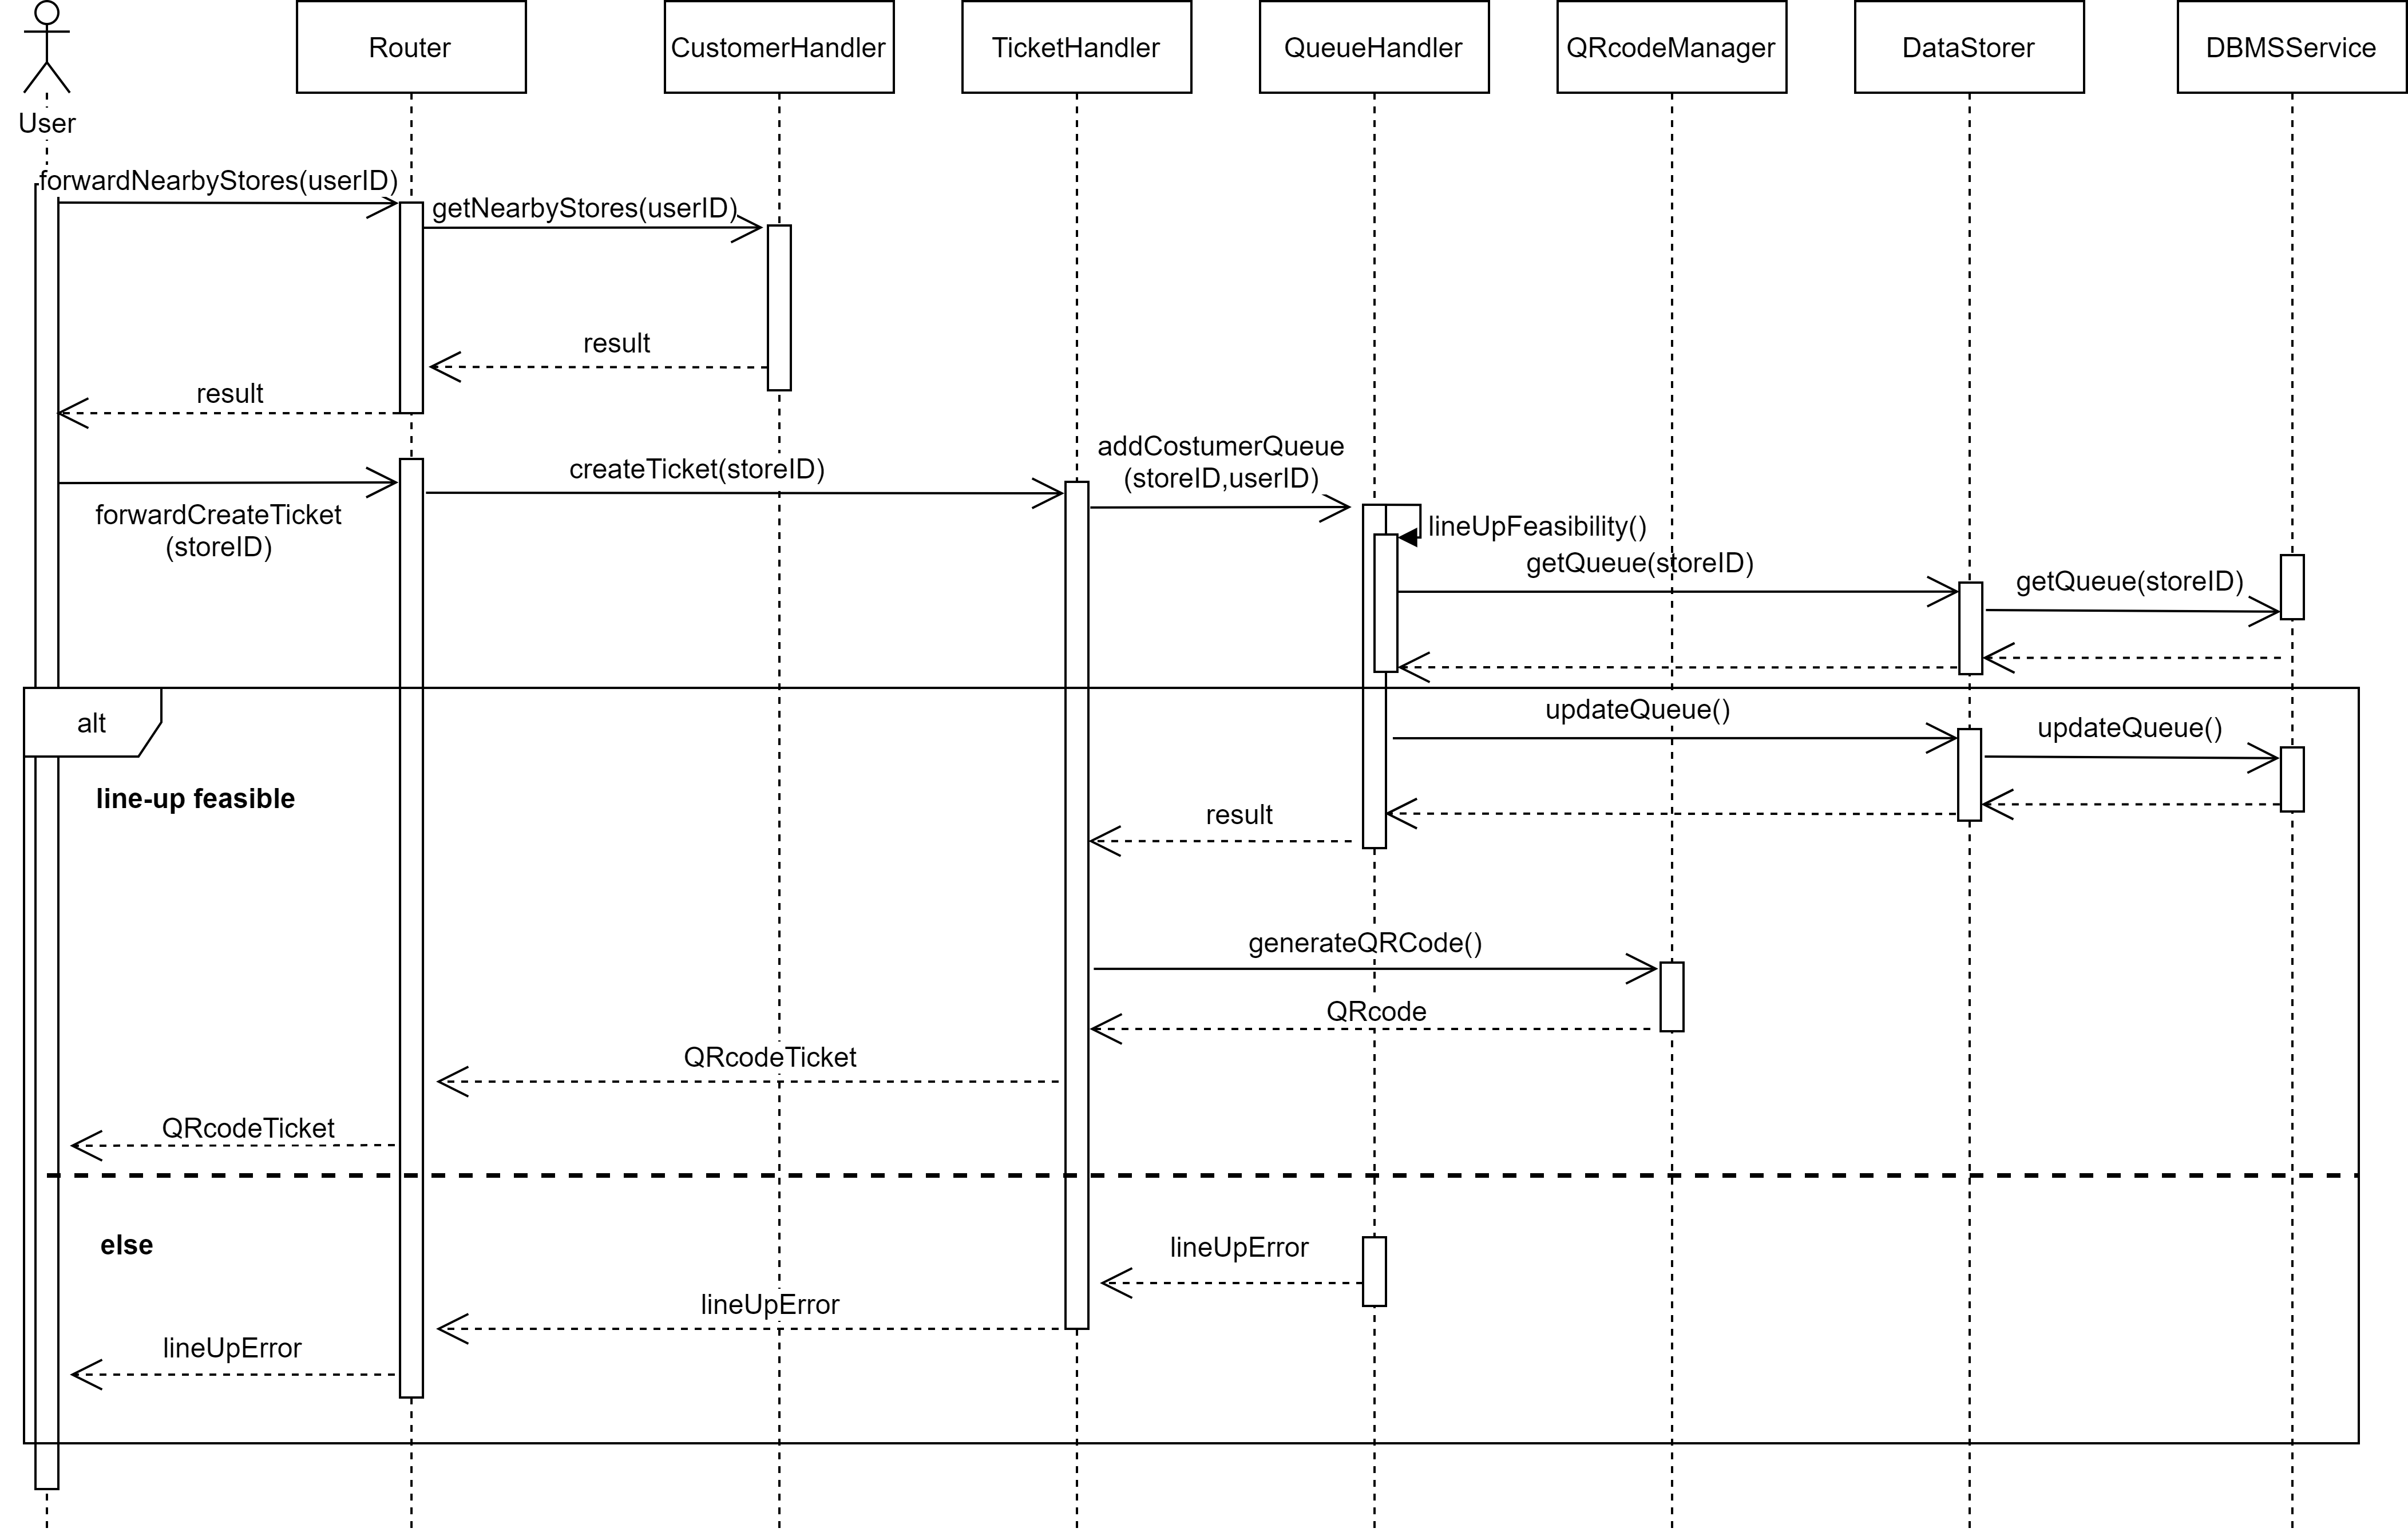
\includegraphics[scale=0.6]{lineupSequence}
		\caption{Line-up sequence diagram}
	\end{figure}
	
	\newpage
	\noindent
	\textbf{Physical Line-up}
	\newline \newline
	Everything starts with the costumer that requires a ticket at the totem outside the store. From this point the flow of events is the same as the previous diagram. The unique difference is that the ticket is not sent to the costumer mobile phone but is returned by the totem, if the costumer is allowed to line-up.
	\bigskip
	
	\begin{figure}[H]
		\centering
		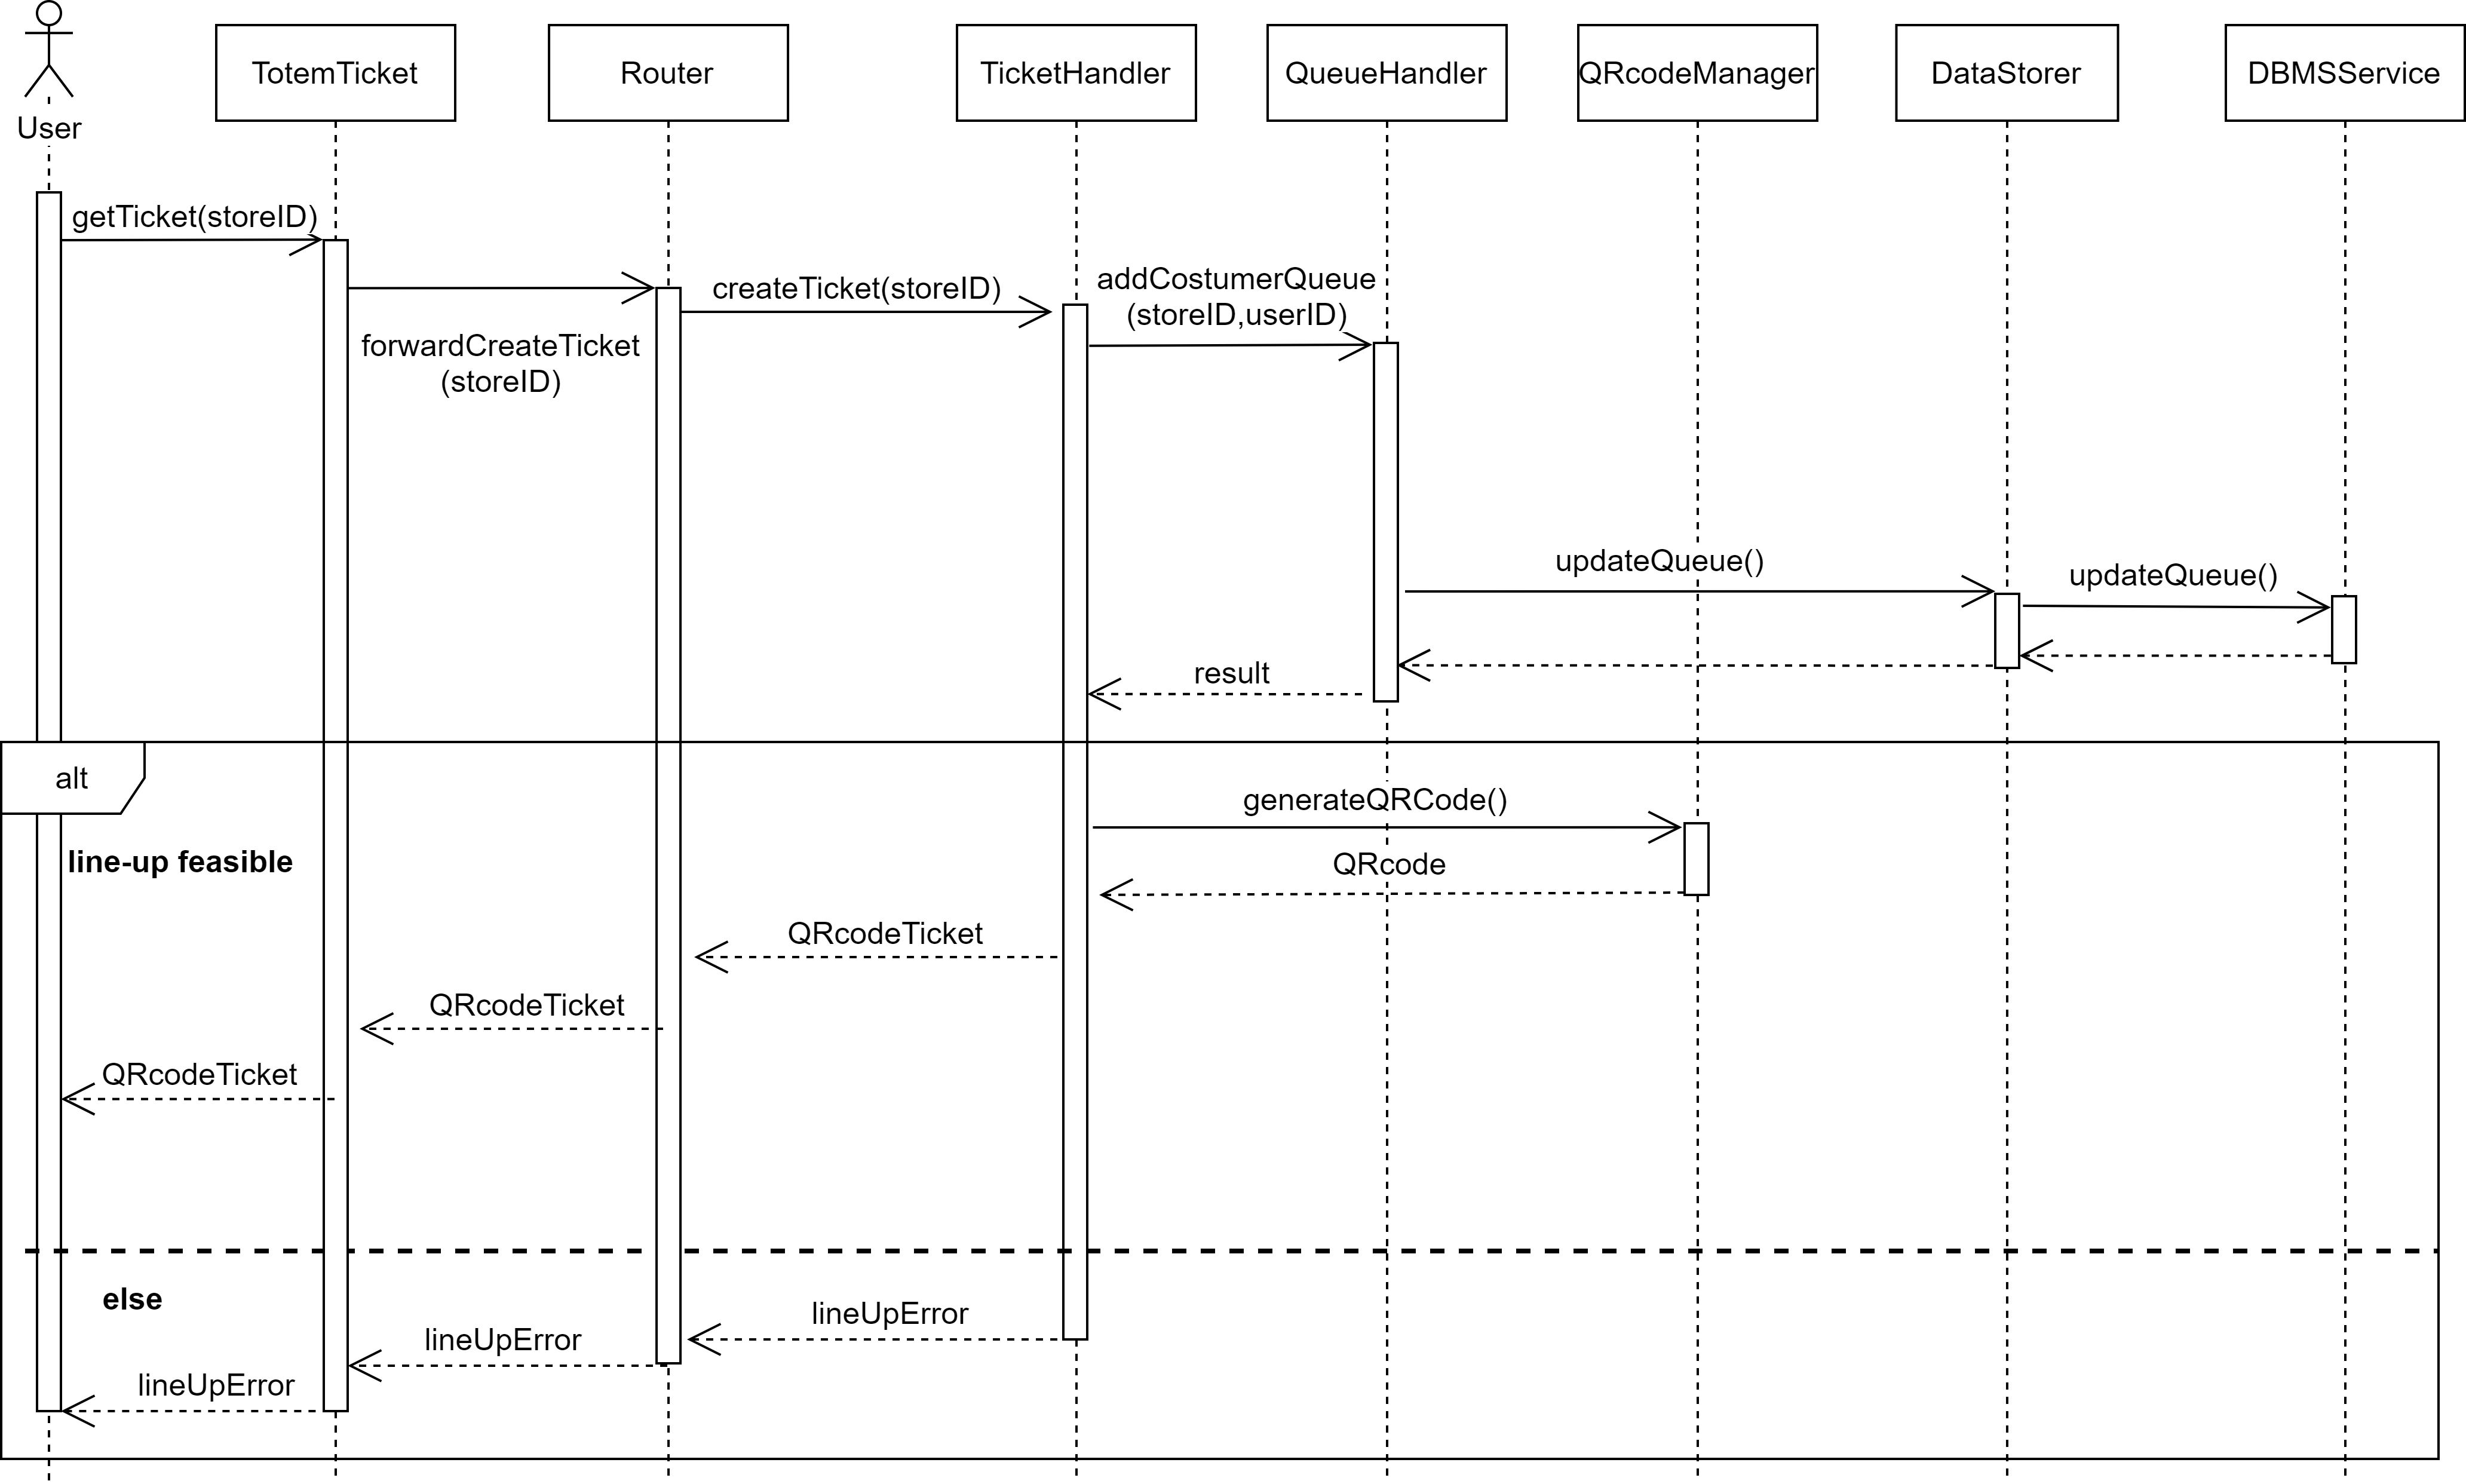
\includegraphics[scale=0.6]{lineupphysicalSequence}
		\caption{Physical Line-up sequence diagram}
	\end{figure}

	\noindent
	\textbf{User enters into the store}
	\newline \newline
	When the user scans his QRcode (either via his mobile app or physical ticket), the request is handled by TicketManager that retrieves the virtual ticket associated with the code. \newline
	Afterwards, QueueHandler checks whether the scanned ticket is actually the next user in the line. 
	If so, the automatic doors are unlocked and the queue is update, otherwise an error message is reported to the user.
	\medskip
	
	\begin{figure}[H]
		\centering
		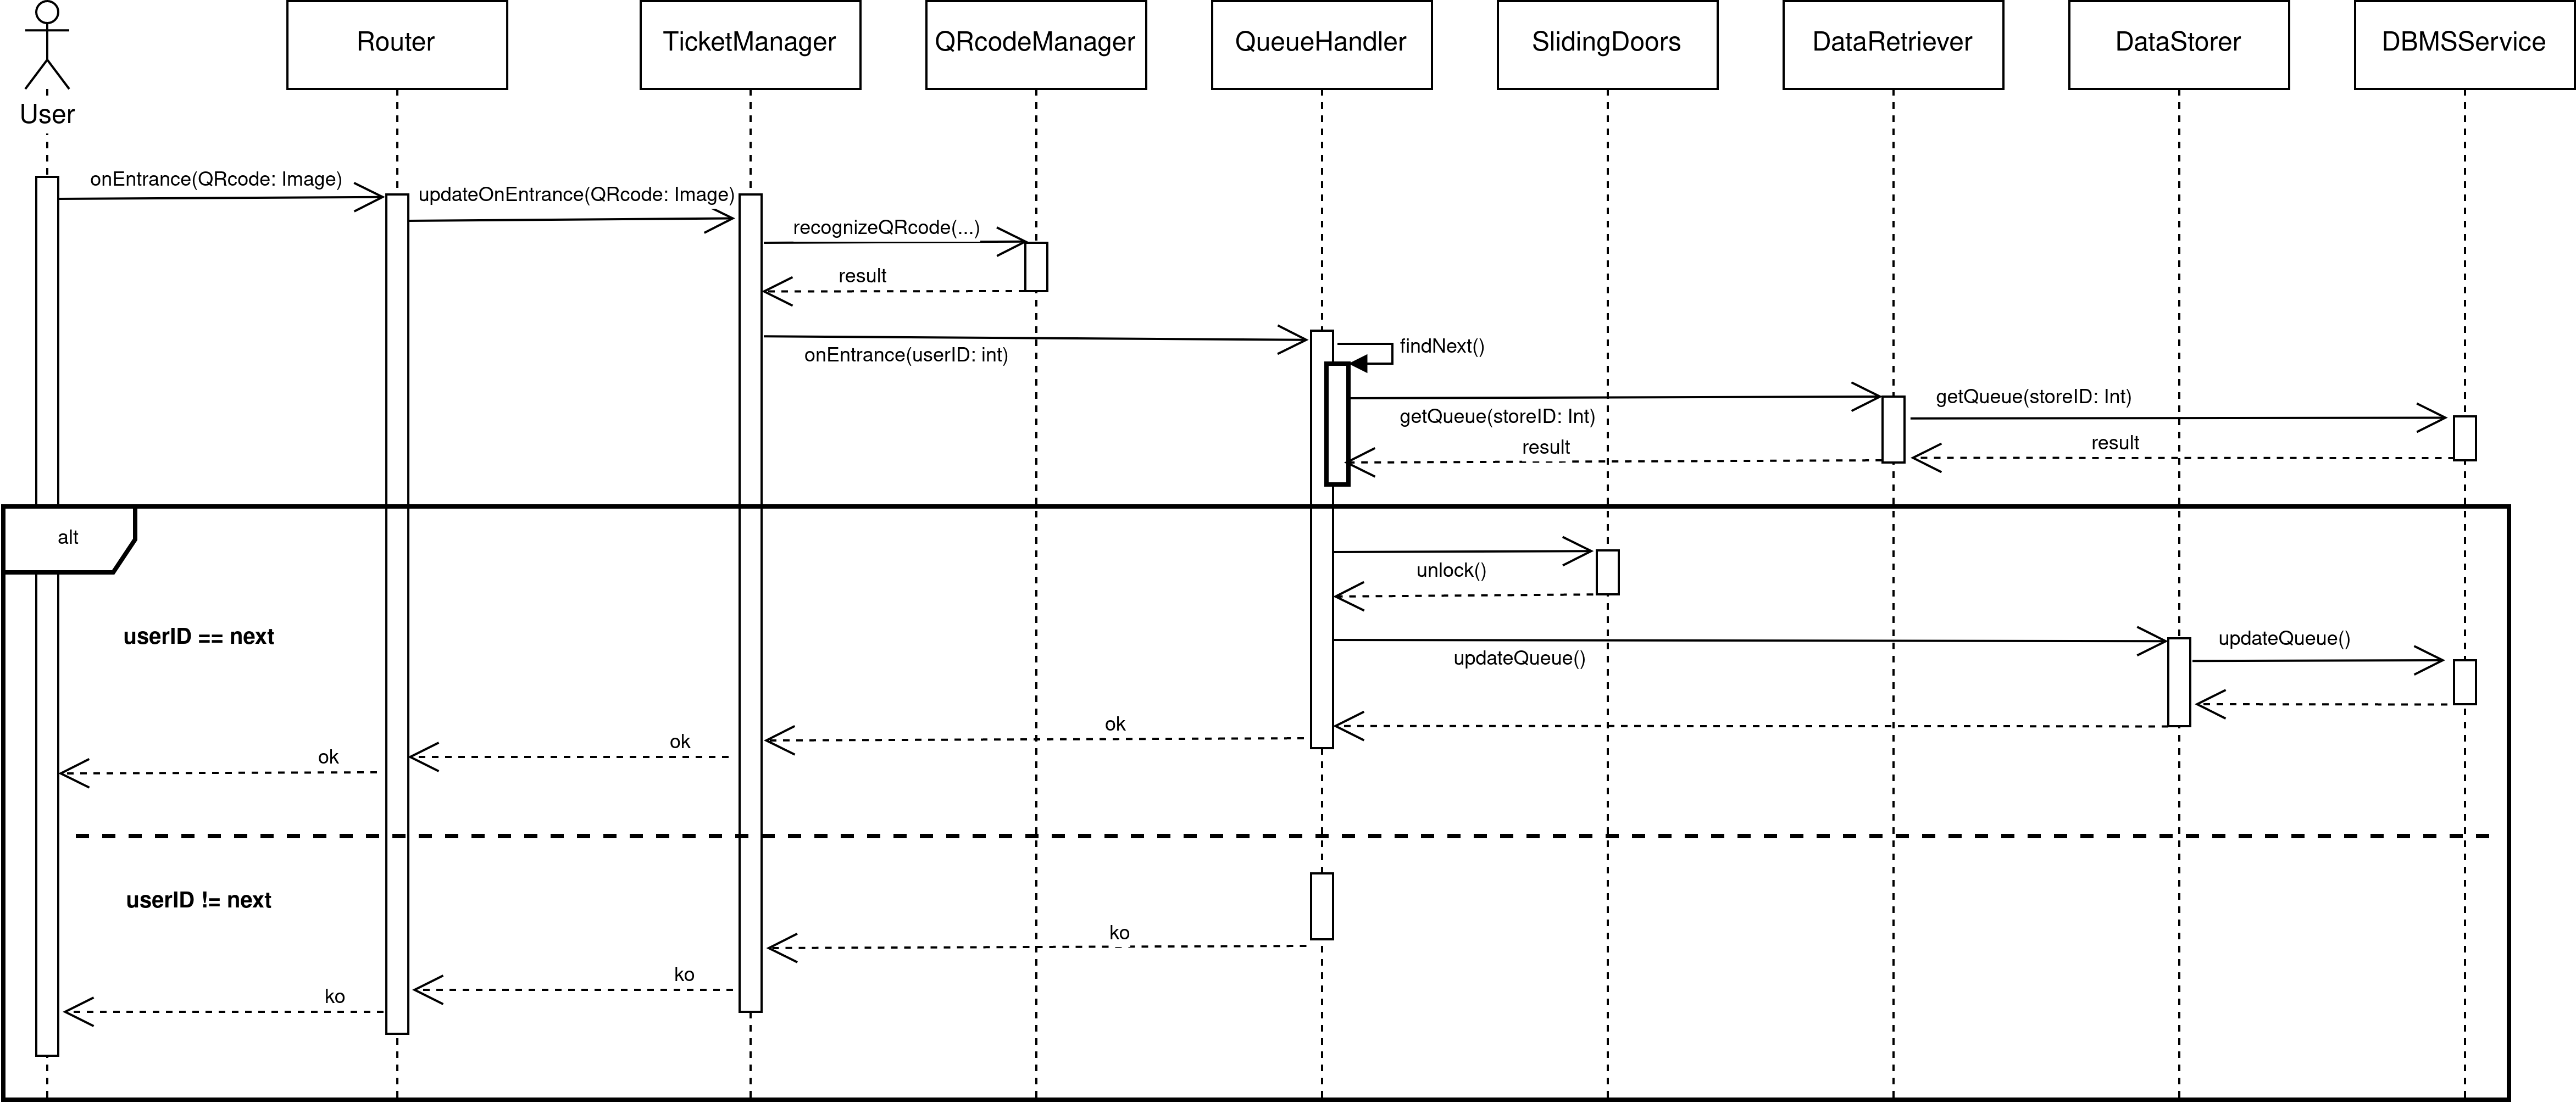
\includegraphics[scale=0.58]{ComponentView/userEnters.png}
		\caption{User enters into the store sequence diagram}
	\end{figure}
	
		\noindent
	\textbf{User books a visit}
	\newline \newline
	The user starts by indicating the item that he is going to buy among the available ones and the preferred time slot. \newline
	The system checks if the visit is feasible (visit overlapping, store opening time etc.) and creates a visit object in the database along with some statistics. An error is reported to the user if some checks went wrong.
	\bigskip \bigskip
	
	\begin{figure}[H]
		\centering
		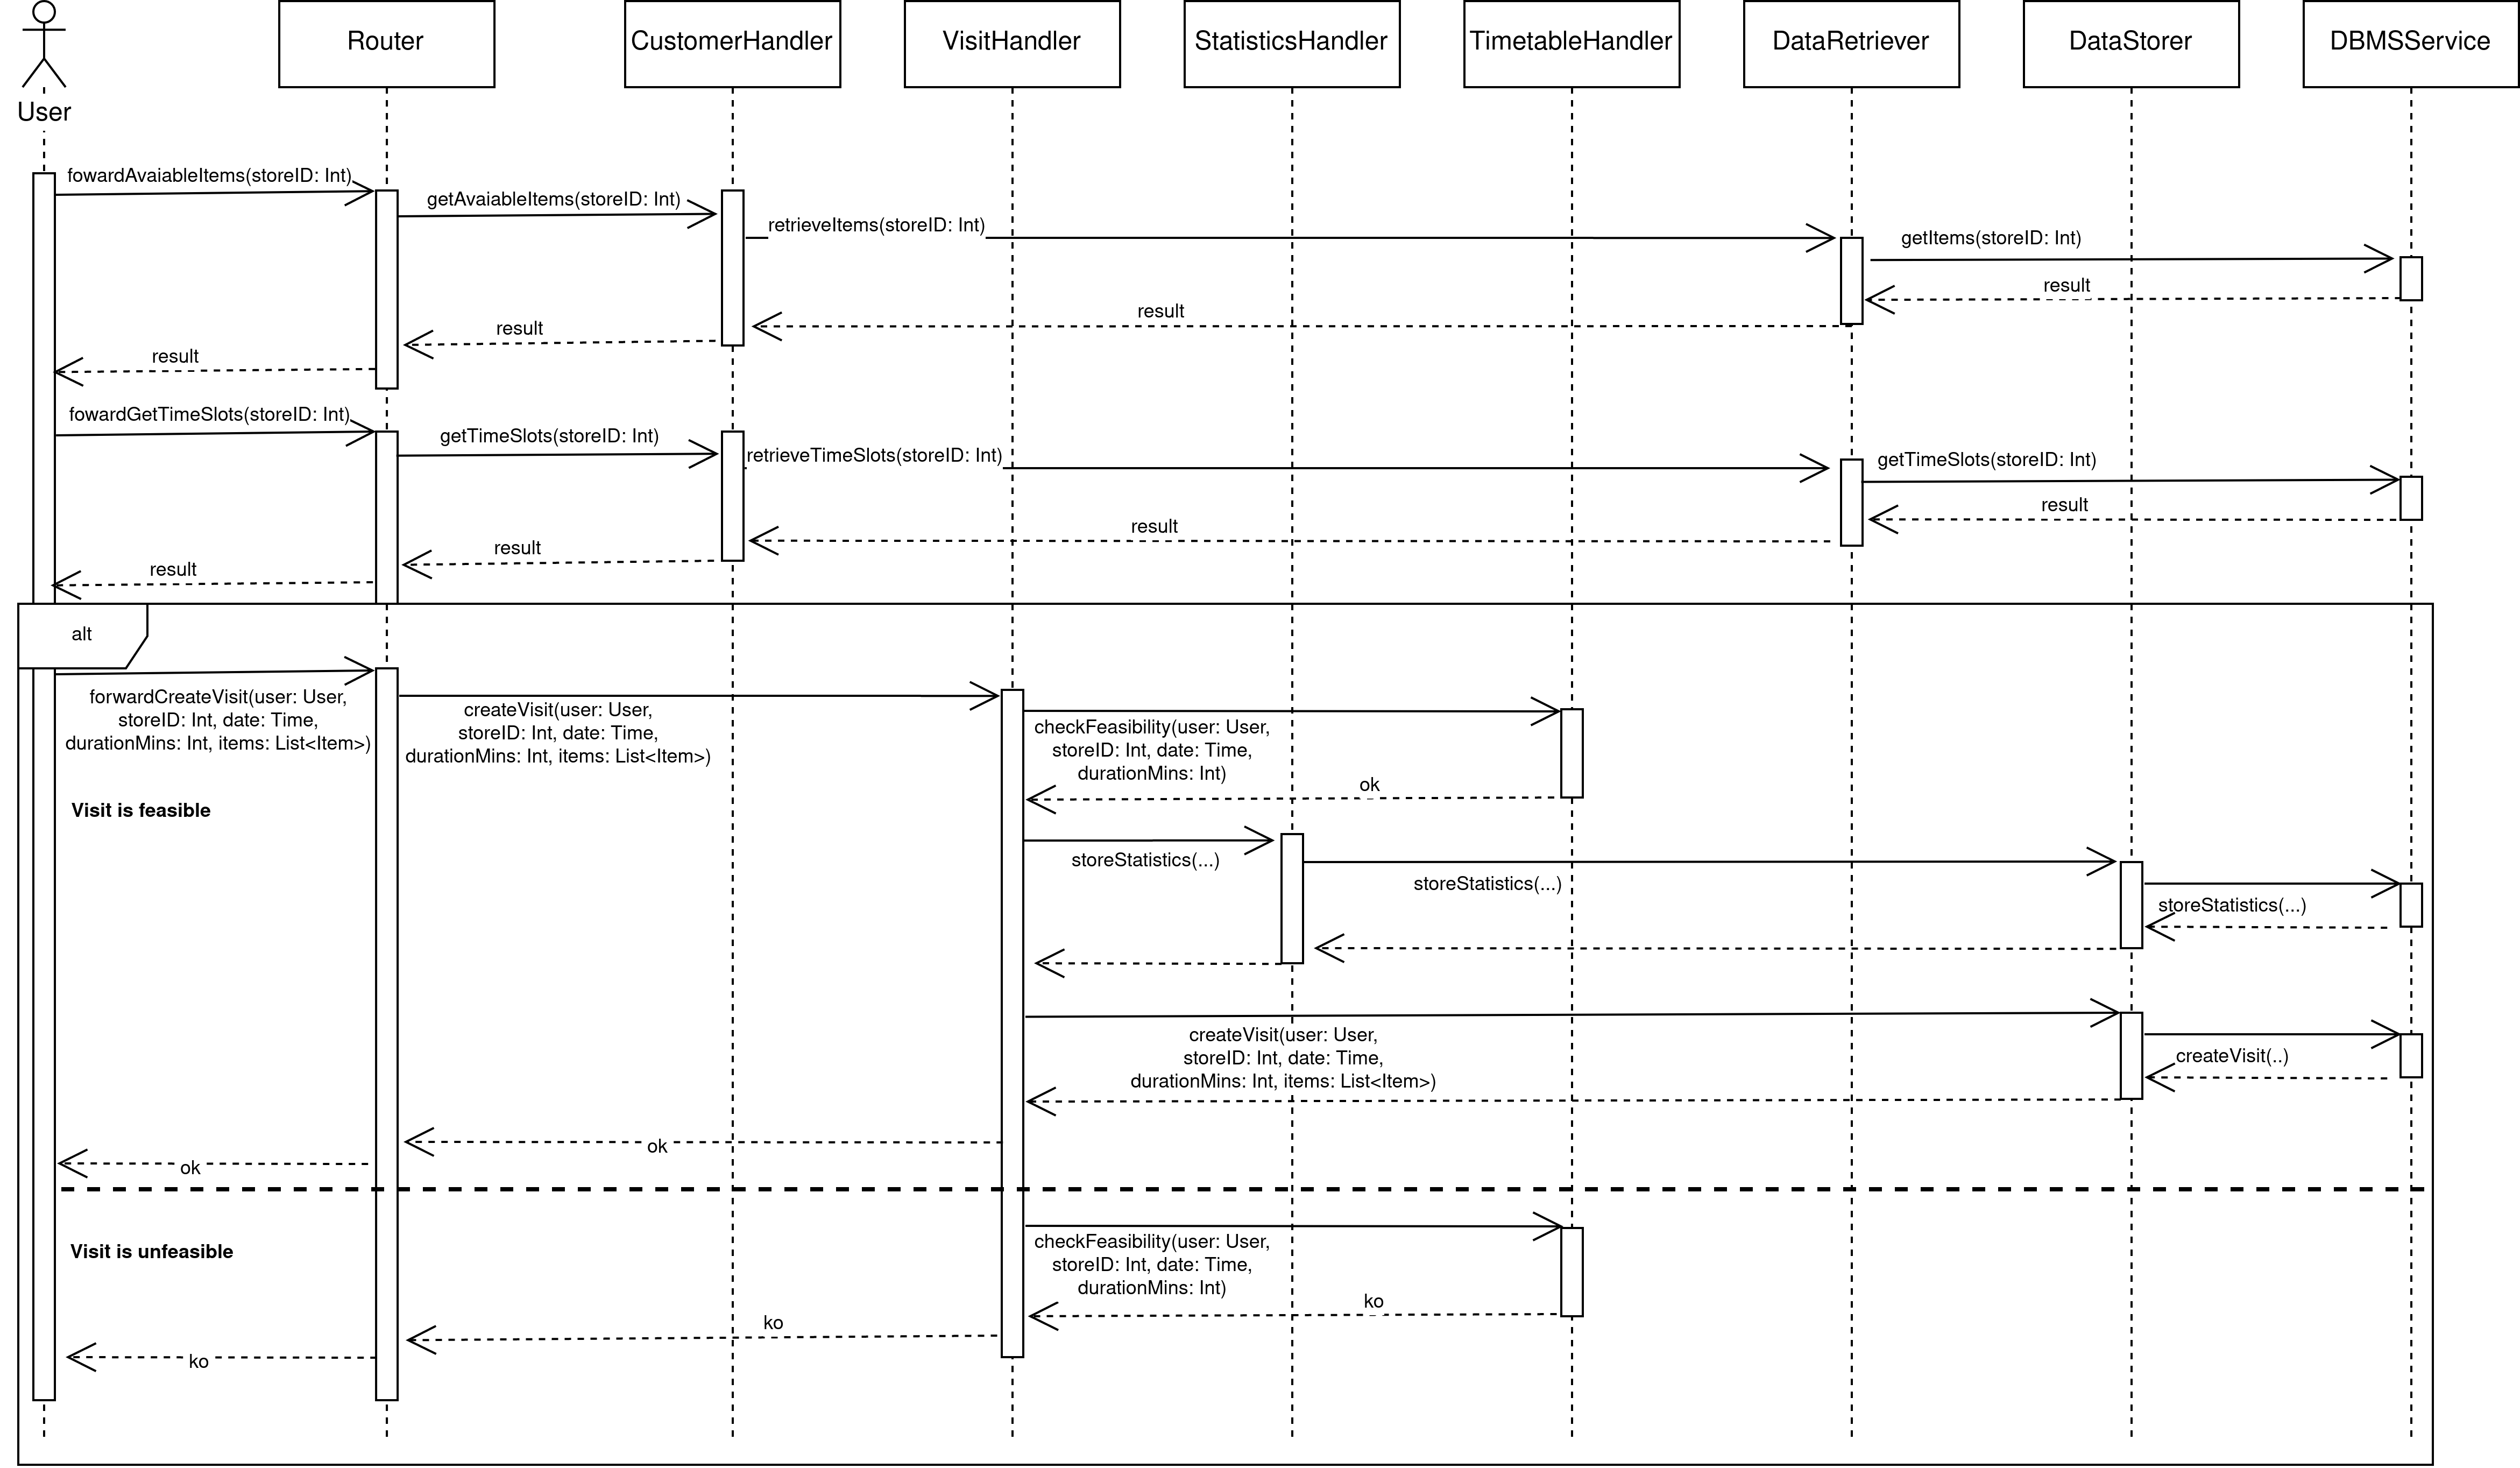
\includegraphics[scale=0.57]{ComponentView/bookAVisitRuntimeView.png}
		\caption{User enters into the store sequence diagram}
	\end{figure}
	
	\newpage
	\noindent
	\textbf{Increase store capacity}
	\newline \newline
	The increase of the capacity starts when the store manager clicks on the correspondent button (this interaction is omitted as said in the section opening). The critical component involved in this scenario is StoreHandler that according to the store data and to the store defined policy (see section 2.4.2 \textit{RASD}), retrieved from the database, decides if the capacity can be increased or not.
	\bigskip \bigskip
	\begin{figure}[H]
		\centering
		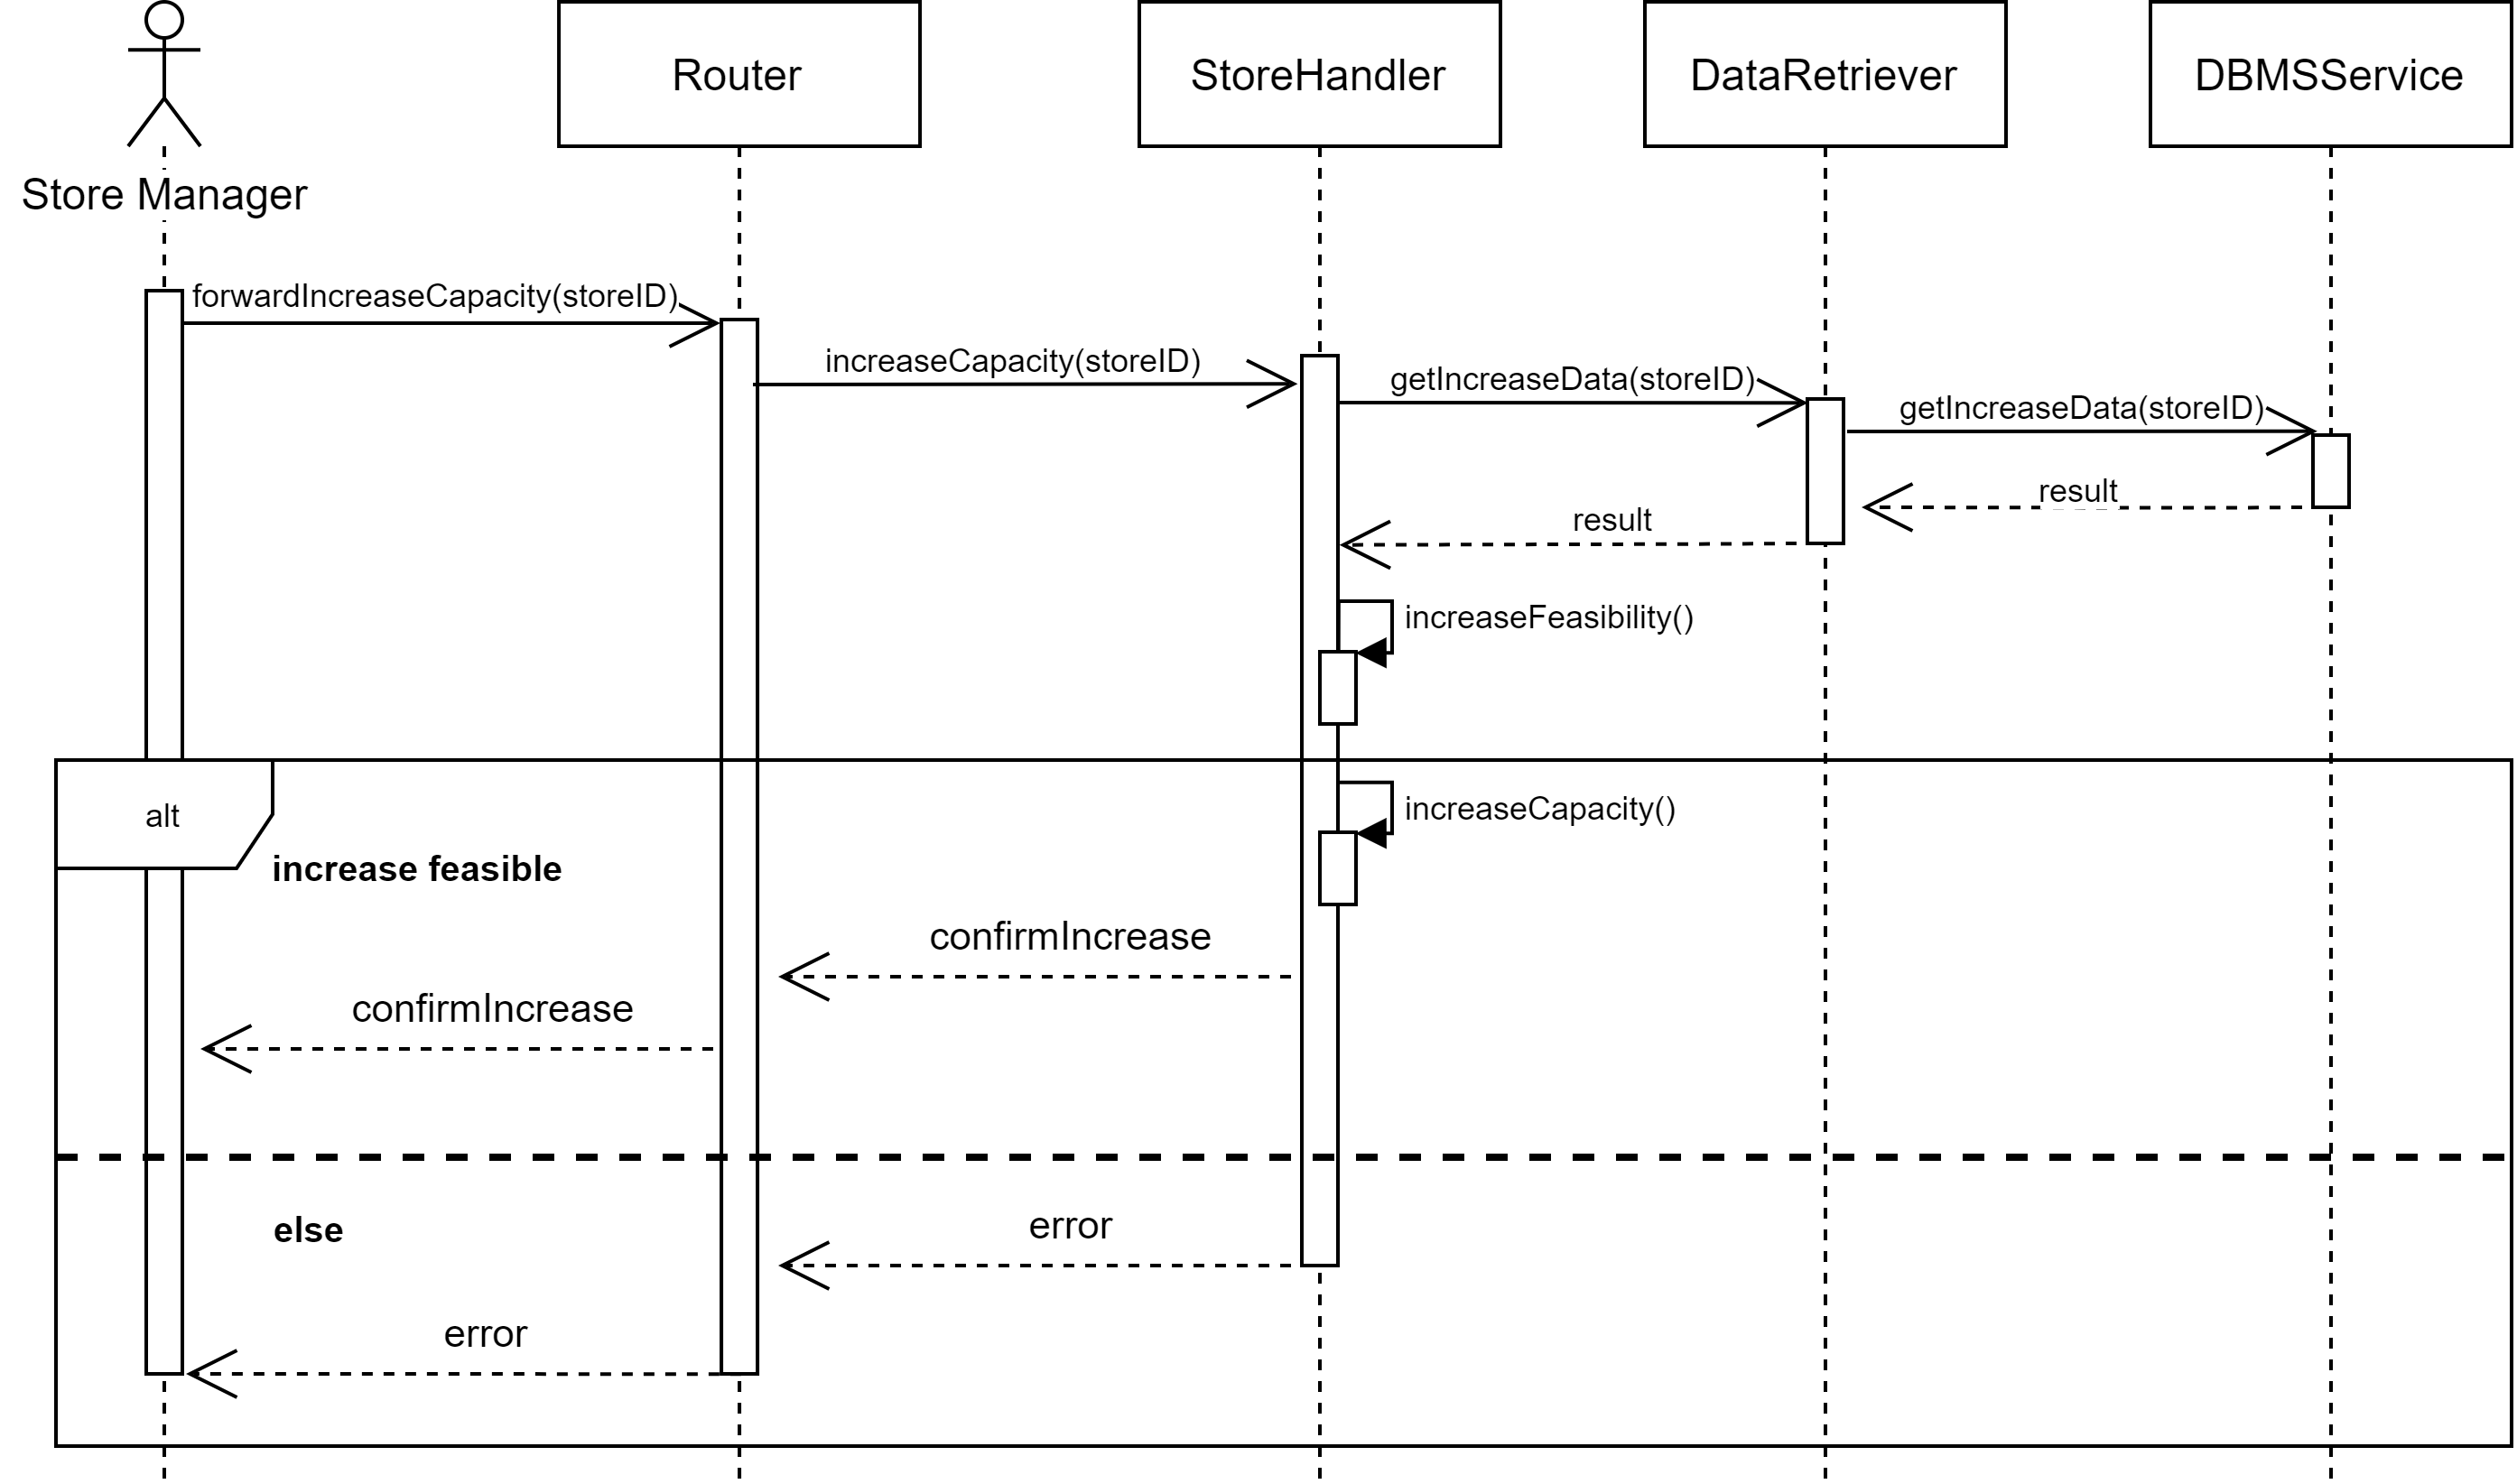
\includegraphics[scale=0.75]{increaseSequence}
		\caption{Increase store capacity sequence diagram}
	\end{figure}
	
	
	\newpage
	
	
	
	\newpage
	\subsection{Selected architectural styles and patterns}
	\medskip
	
	\subsubsection{High level architecture}
	The CLup system adopts a 3 tier architecture. 
	How it works and how it is mapped on the system components is explained in section 2.1, where the reader is invited for further explanations.
	
	\subsubsection{Client-Server}
	The client-server paradigm is the one that better fits the CLup system.
	\\The client is represented by users devices, smartphones for costumers and Personal Computers for store managers. In particular the chosen style is thin client, in fact, all the computations are done server side, the client has only to display something to the user and to catch interactions.
	\\On the other side, the server is represented by the Business Logic tier and the Data tier. As just said, the server does all the computations and handles all the requests that come from the client. 
	
	\subsubsection{MVC - Model View Controller}
	Another important pattern implemented in the CLup software system is the Model-View-Controller.
	The pattern is mapped along the client and the server. 
	The View is located in the client. Users devices have the unique task of display information and allow interactions with the system, as said in the previous paragraph.
	\\The Controller and the Model are located server-side.
	The Controller is composed by all the components of the Application Server except the DataManger subsystem. These components handle clients (View) requests and update the Model data. 
	\\The Model is represented by the DataManger subsystem and by the Data tier. The first is the link between the controller and the Database where all the data are stored, as explained in section 2.2.
	\newline
	\newline
	\newline
	In the following diagram is shown how the three architectural patterns just explained are integrated with each other.
	\bigskip
	\begin{figure}[H]
		\centering
		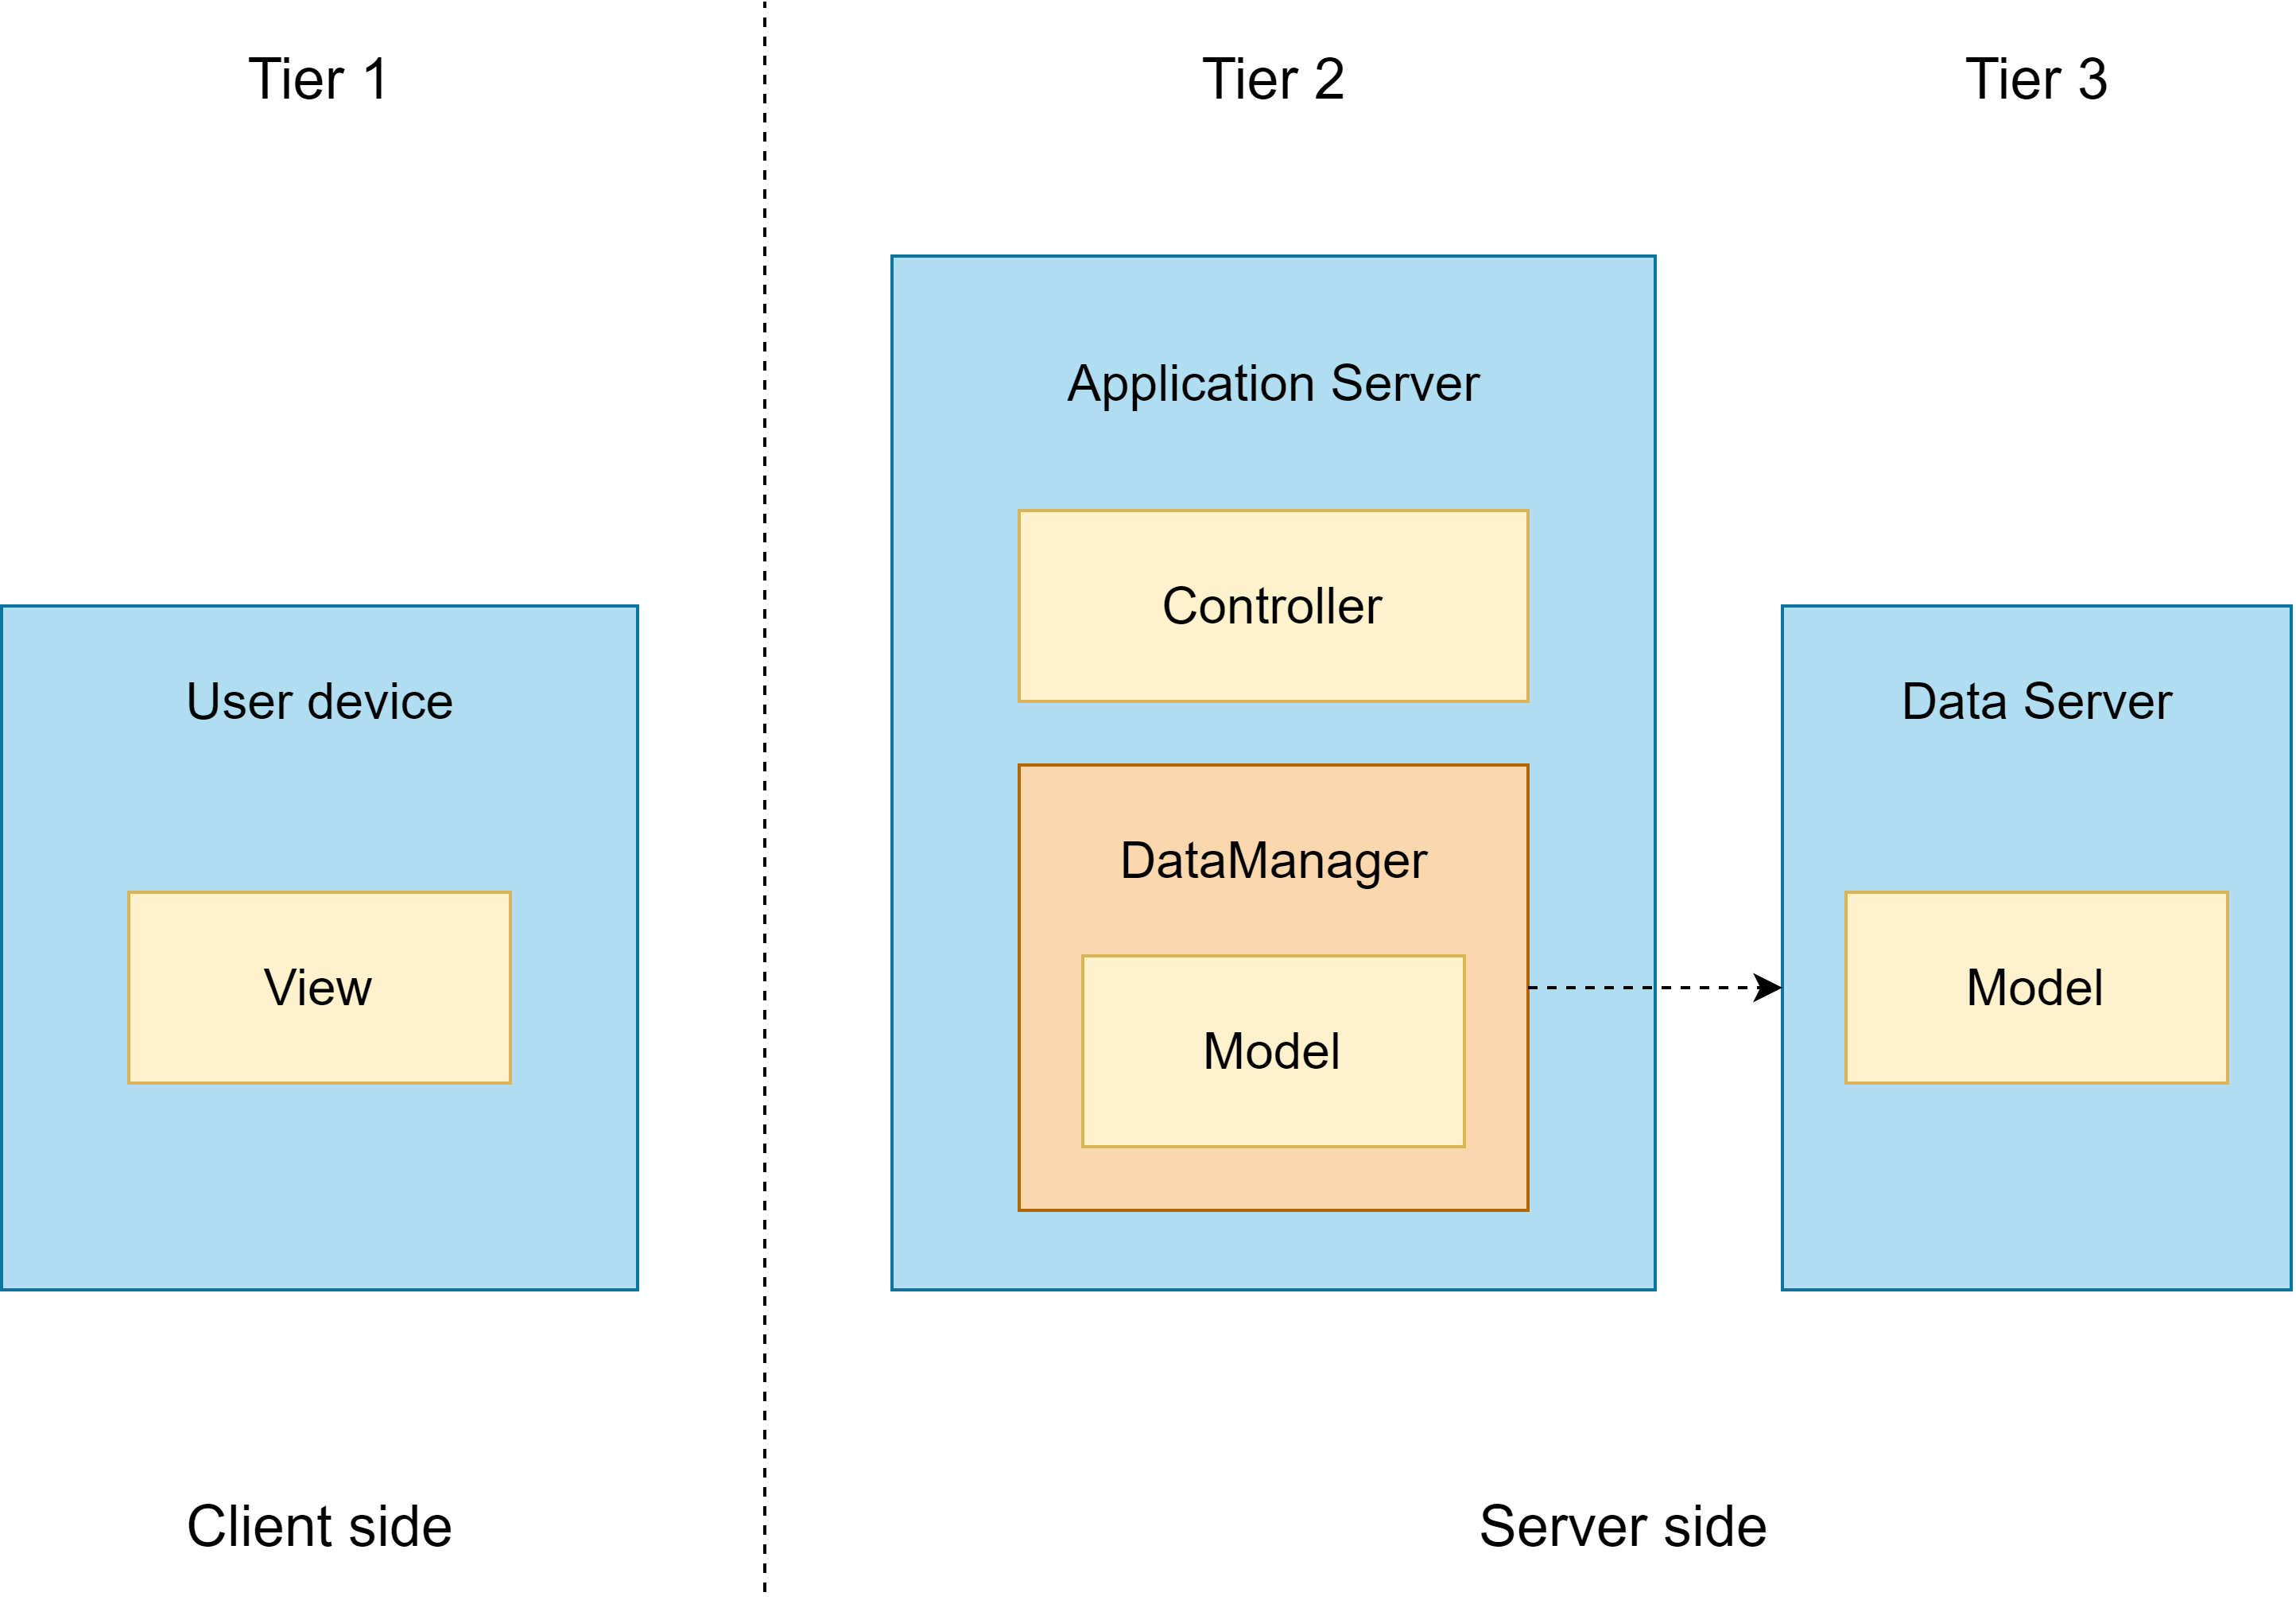
\includegraphics[scale=0.8]{MVC}
		\caption{}
	\end{figure}
	
	
	\subsection{Algorithms and data structures}
	\subsubsection{Queue}
	One of the challenges faced when designing the system is how to properly integrate, in the same virtual queue, in person customers, CLup users that lined up with the mobile app and CLup users that booked a visit. \newline
	In order to manage the line as smoothly as possible, booked visits are being treated similarly to a normal line up. \newline
	\textbf{Visit Handler} needs a routine that, once the time of the booked visit is reached, inserts our booked user in the queue. \newline
	This insertion however is not like other insertions because the user is virtually inserted as the first of our queue.\newline \newline
	In order to achieve this behavior and ease the integration between different type of users, the data structure of the queue should be a  \textit{priority-driven FIFO queue}. \newline
	The ordering policy of the queue is the following: entities are ordered firstly based on their priority (i.e. no entities can be preceded by an entity of lower priority) and secondly in a \textit{first come first served} manner (i.e. FIFO ordering between entities of the same priority). \newline \newline
	This design is exploited as follows: given two priority values \textbf{H} and \textbf{L} (with priority(H) $>$ priority(L)), requests to line up (either physically or through the CLup app) are served by inserting the user in the queue with the L priority (this creates a plain FIFO queue if only this types of requests are present). \newline
	Instead, booked visits are inserted in the queue with the H priority, placing them before other L entities. \newline \newline
	The following example shows the queue logic explained above.\newline 
	The queue is intended to be read from left to right (i.e. the leftmost item is the first of the queue). \newline
	
		\begin{figure}[h!] 
		\centering
		\subfloat[Initial state of the queue]
		{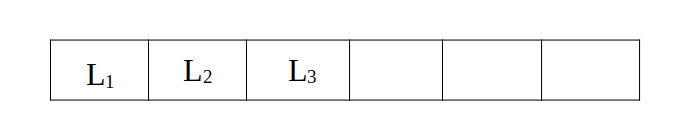
\includegraphics[width=.42\textwidth]{ComponentView/queue1}}
		\qquad\qquad
		\subfloat[H1 enters the queue]
		{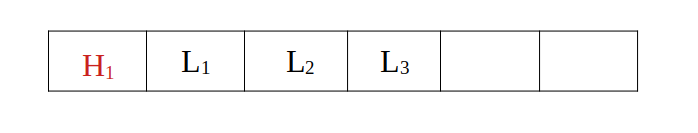
\includegraphics[width=.42\textwidth]{ComponentView/queue2}}
		\qquad\qquad
		\end{figure}
	
		\begin{figure}[h!] 
		\centering
		\subfloat[L4 enters the queue]
		{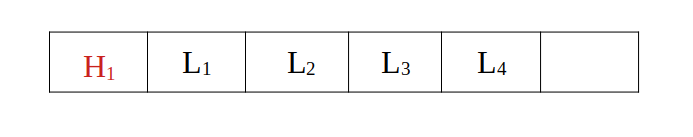
\includegraphics[width=.42\textwidth]{ComponentView/queue3}}
		\qquad\qquad
		\subfloat[H2 enters the queue]
		{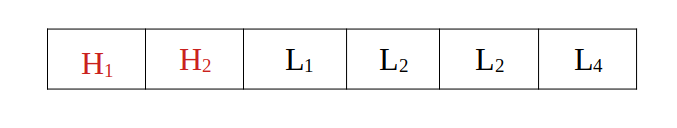
\includegraphics[width=.42\textwidth]{ComponentView/queue4}}
		\qquad\qquad
		\end{figure}
	 \noindent
	 With this policy, once a visit time has come, the related user is inserted in the queue with the H priority making him the first (or among the first if many booked users are in queue) to enter as soon as a customer exits the store. \newline
	 This queue can be implemented in several ways, two of them are:
	 \begin{itemize}
	 	\item Two different FIFO queues, one for the H priority and one for the L. The next() method of the queue could be as follows:
	 	\begin{lstlisting}[language=java]
	 	/*Java example: consider H and L declared as follows
	 	import java.util.LinkedList<E>
	 	LinkedList<Ticket> H = new LinkedList();
	 	LinkedList<Ticket> L = new LinkedList(); */
	 	
	 	public Ticket next() {
	 		if (H.peekFirst() != null) return H.pollFirst();
	 		return L.poolFirst();
	 	}
	 	\end{lstlisting}
	 	\item A unique list/array where every item has a flag that specifies his priority. Insert operation will put items in the structure as described by the logic explained above while the next() function will simply retrieve the first element.
	 \end{itemize}
	
	\subsubsection{Timetable}
	When the system is handling the generation of a visit it has to check whether or not the user has other visits that would overlap with the new one. \newline
	This can be done by retrieving all user future booked visits and using the following function checkOverlapping(). \newline
	Note that the function's inputs are Time objects previously defined in the UML class diagram. \newline
	
	 \begin{lstlisting}[language=java]
	//Java example
	import java.util.Date;
	
	//true if t1 and t2 are overlapping, false otherwise	
	public boolean checkOverlapping(Time t1, Time t2) {
		if (t1.getDate().equals(t2.getDate())) {
			return (t1.getStartingHour() <= t2.getEndingHour() &&
				t2.getStartinHour() <= t1.getEndingHour());
		} 
		return false;
	}
	\end{lstlisting}
	\newpage
	\section{User Interface Design}
	This chapter aims to give a general idea of the user interface, both of the costumer mobile application and the store manager webapp. 
	This is done by means of mockups and UX diagrams.
		
		\subsection{Mockups}
		In the design process of the user interface the main guideline was the Requirement R2 (\textit{The user and manager applications are clear, intuitive and simple to use} - RASD). Therefore, the screen contains only the necessary components and the interaction with them is limited to a few of intuitive form and buttons.
		\\The presented mockups cover almost the totality of the screens you will find on the completed user interface. They show only the components needed to address the CLup goals, buttons such as "return to the previous screens" are not usually taken into account.
		\\\\\\
			\subsubsection{Mobile Application Mockups}
			\bigskip \bigskip
			\begin{figure}[h!] 
				\centering
				\subfloat[Sign-in screen]
				{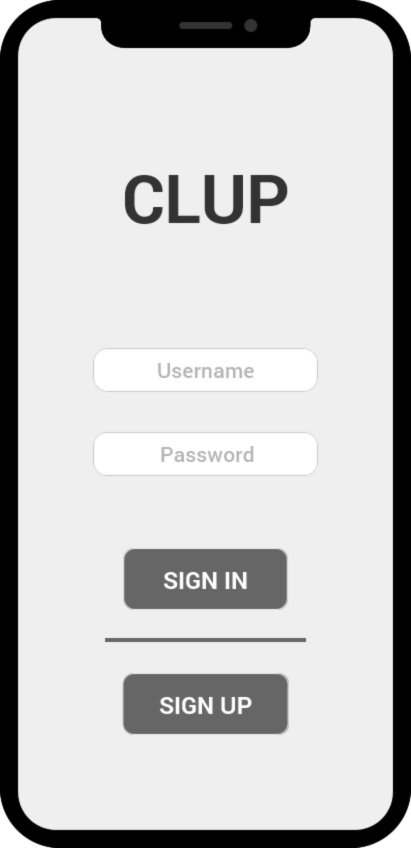
\includegraphics[width=.25\textwidth]{Mockups/signIn}}
				\qquad\qquad
				\subfloat[Sign-up screen]
				{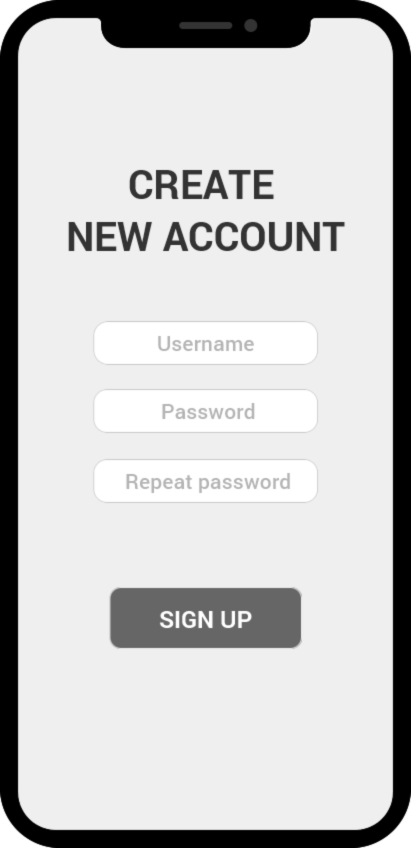
\includegraphics[width=.25\textwidth]{Mockups/signUp}}
				\qquad\qquad
				\subfloat[Store selection/booking check screen]
				{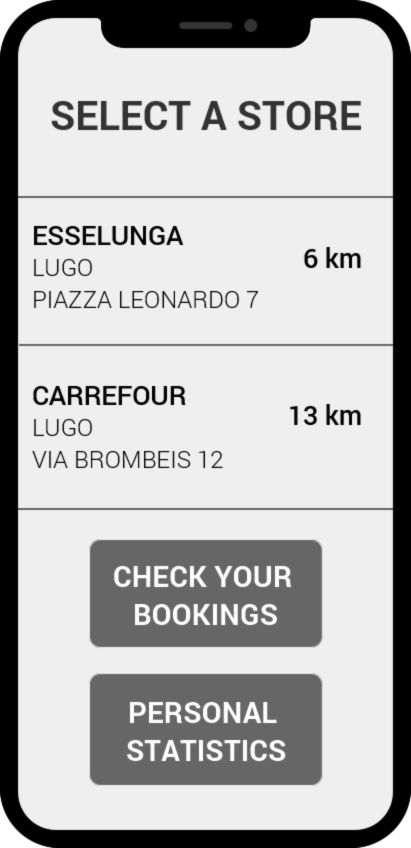
\includegraphics[width=.25\textwidth]{Mockups/selectStore}} 
			\end{figure}
		
			\newpage
			\textbf{}\\
			\bigskip \bigskip \bigskip
			\begin{figure}[h!]\ContinuedFloat
				\centering
				\subfloat[Booking check screen]
				{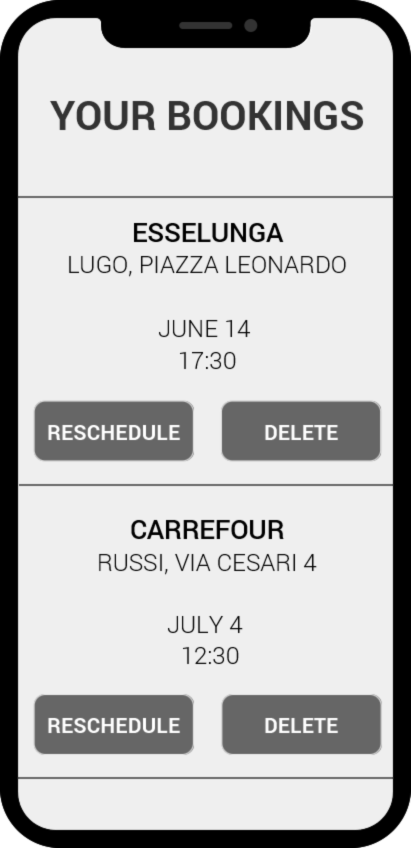
\includegraphics[width=.25\textwidth]{Mockups/bookingCheck}}
				\qquad\qquad
				\subfloat[Store available actions screen]
				{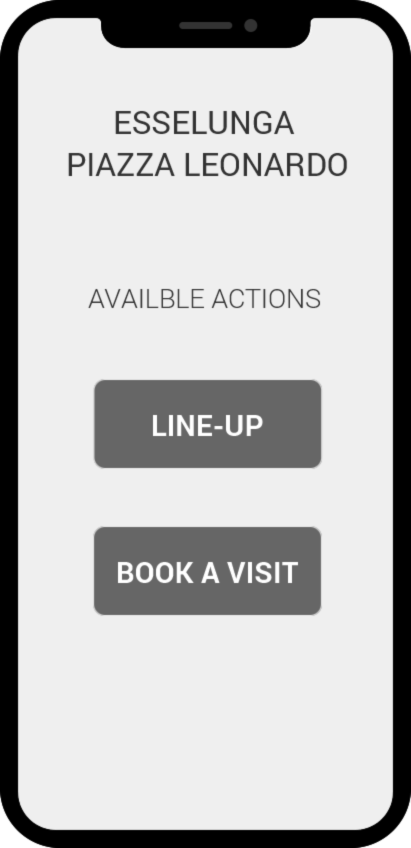
\includegraphics[width=.25\textwidth]{Mockups/storeAvailableActions}}
				\qquad\qquad
				\subfloat[Queue status screen]
				{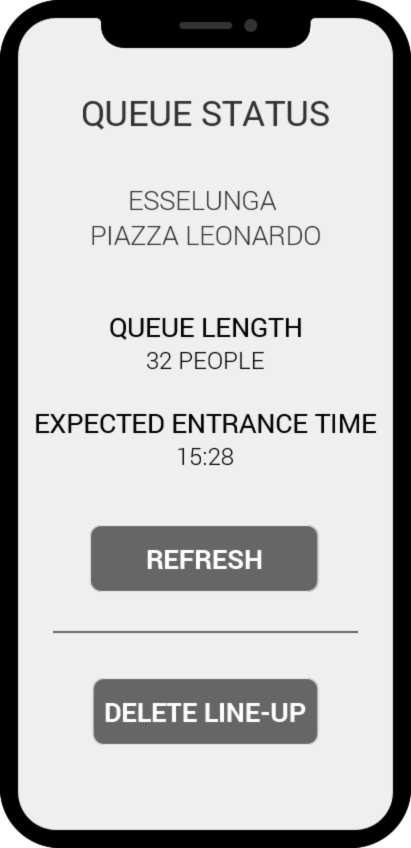
\includegraphics[width=.25\textwidth]{Mockups/queueStatus}} 
				
				\bigskip \bigskip \bigskip
				
				\subfloat[Book a visit screen]
				{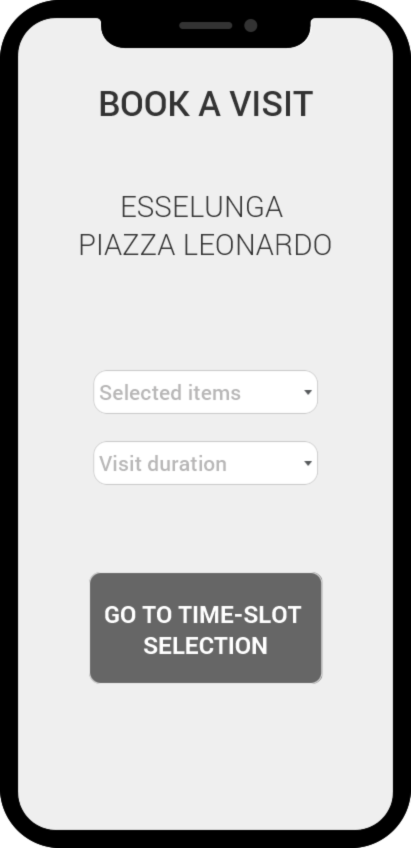
\includegraphics[width=.25\textwidth]{Mockups/bookVisit}}
				\qquad\qquad
				\subfloat[Time-slot selection screen]
				{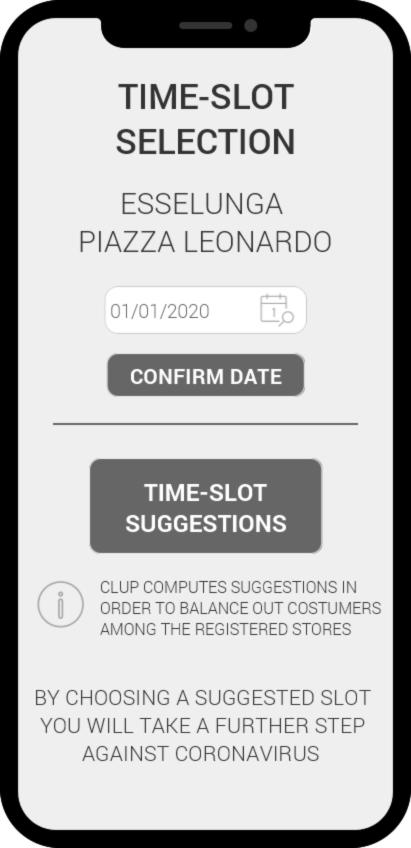
\includegraphics[width=.25\textwidth]{Mockups/timeSlotSelection}}
				\qquad\qquad
				\subfloat[CLup notification]
				{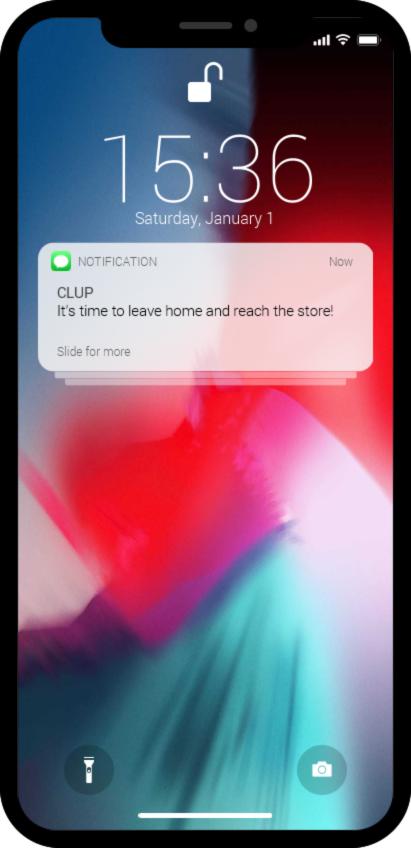
\includegraphics[width=.25\textwidth]{Mockups/notification}} 
			\end{figure}
		
			\newpage
			\subsubsection{WebApp Mockups}
			\bigskip
		
			\begin{figure}[H]
				\centering
				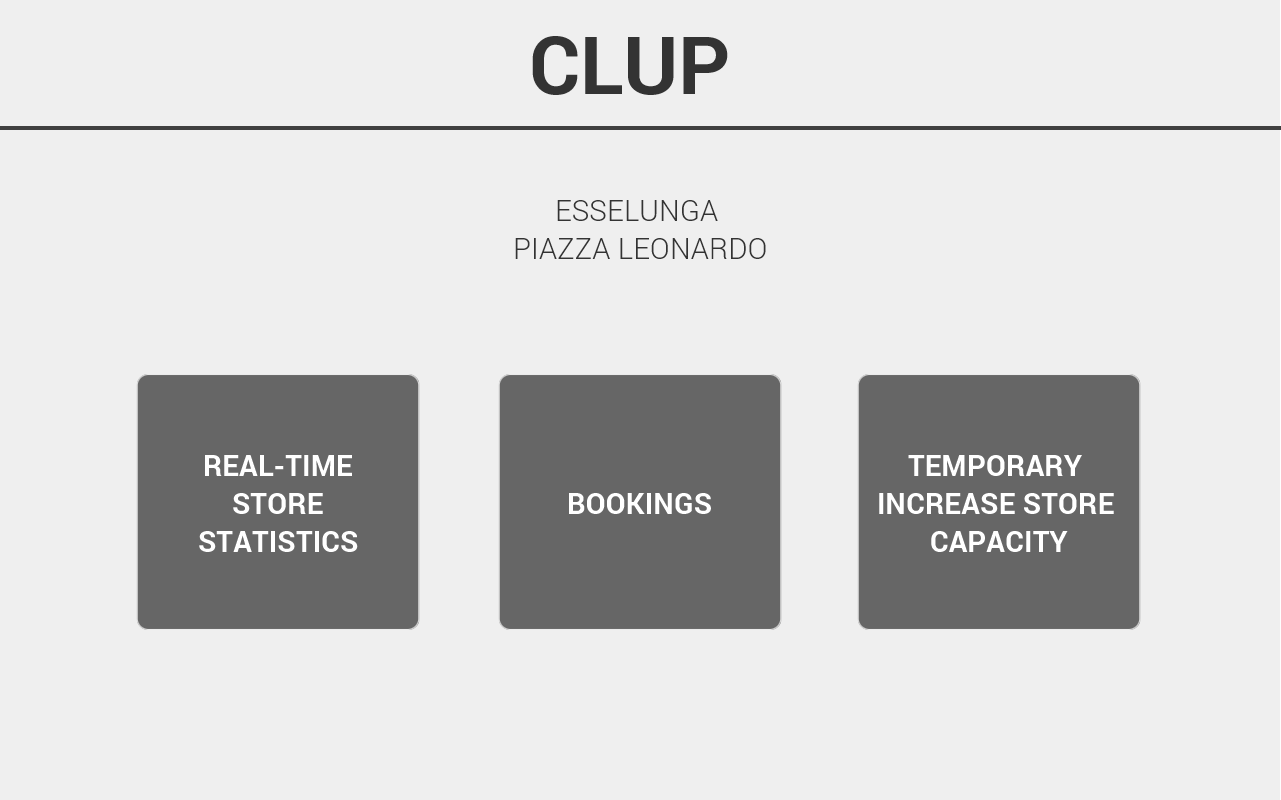
\includegraphics[scale=0.3]{Mockups/webAppHome}
				\caption{Home screen}
				\label{fig:homeScreen}
			\end{figure}
			\bigskip
			
			\begin{figure}[H]
				\centering
				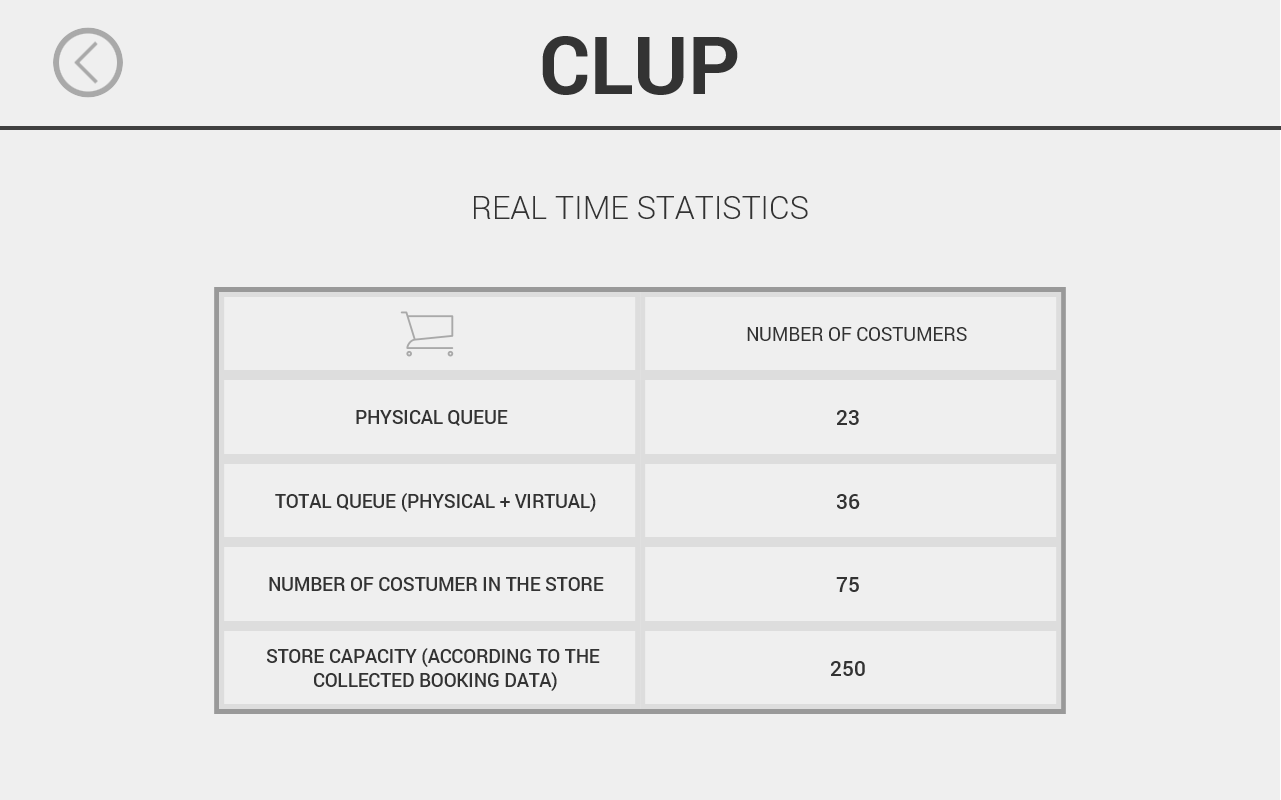
\includegraphics[scale=0.489]{Mockups/storeStatistics}
				\caption{Store statistics screen}
				\label{fig:Storestatisticsscreen}
			\end{figure}
		
			
			\begin{figure}[H]
				\centering
				\includegraphics[scale=0.3]{Mockups/storeBookings}
				\caption{Store bookings screen}
				\label{fig:ManagerHomeMockup}
			\end{figure}
		
		\newpage
		\subsection{UX diagrams}
		The chapter ends with two UX diagrams. They show the general flow of the screens giving more details on the user experience. "General" because some link between screens where omitted, like the "return" from a screen to the previous.
		
		\begin{figure}[H]
			
\includegraphics[scale=0.7]{UX diagrams/legend}
			\label{fig:MobileAppUXdiagram}
		\end{figure}
		\begin{figure}[H]
			\centering
			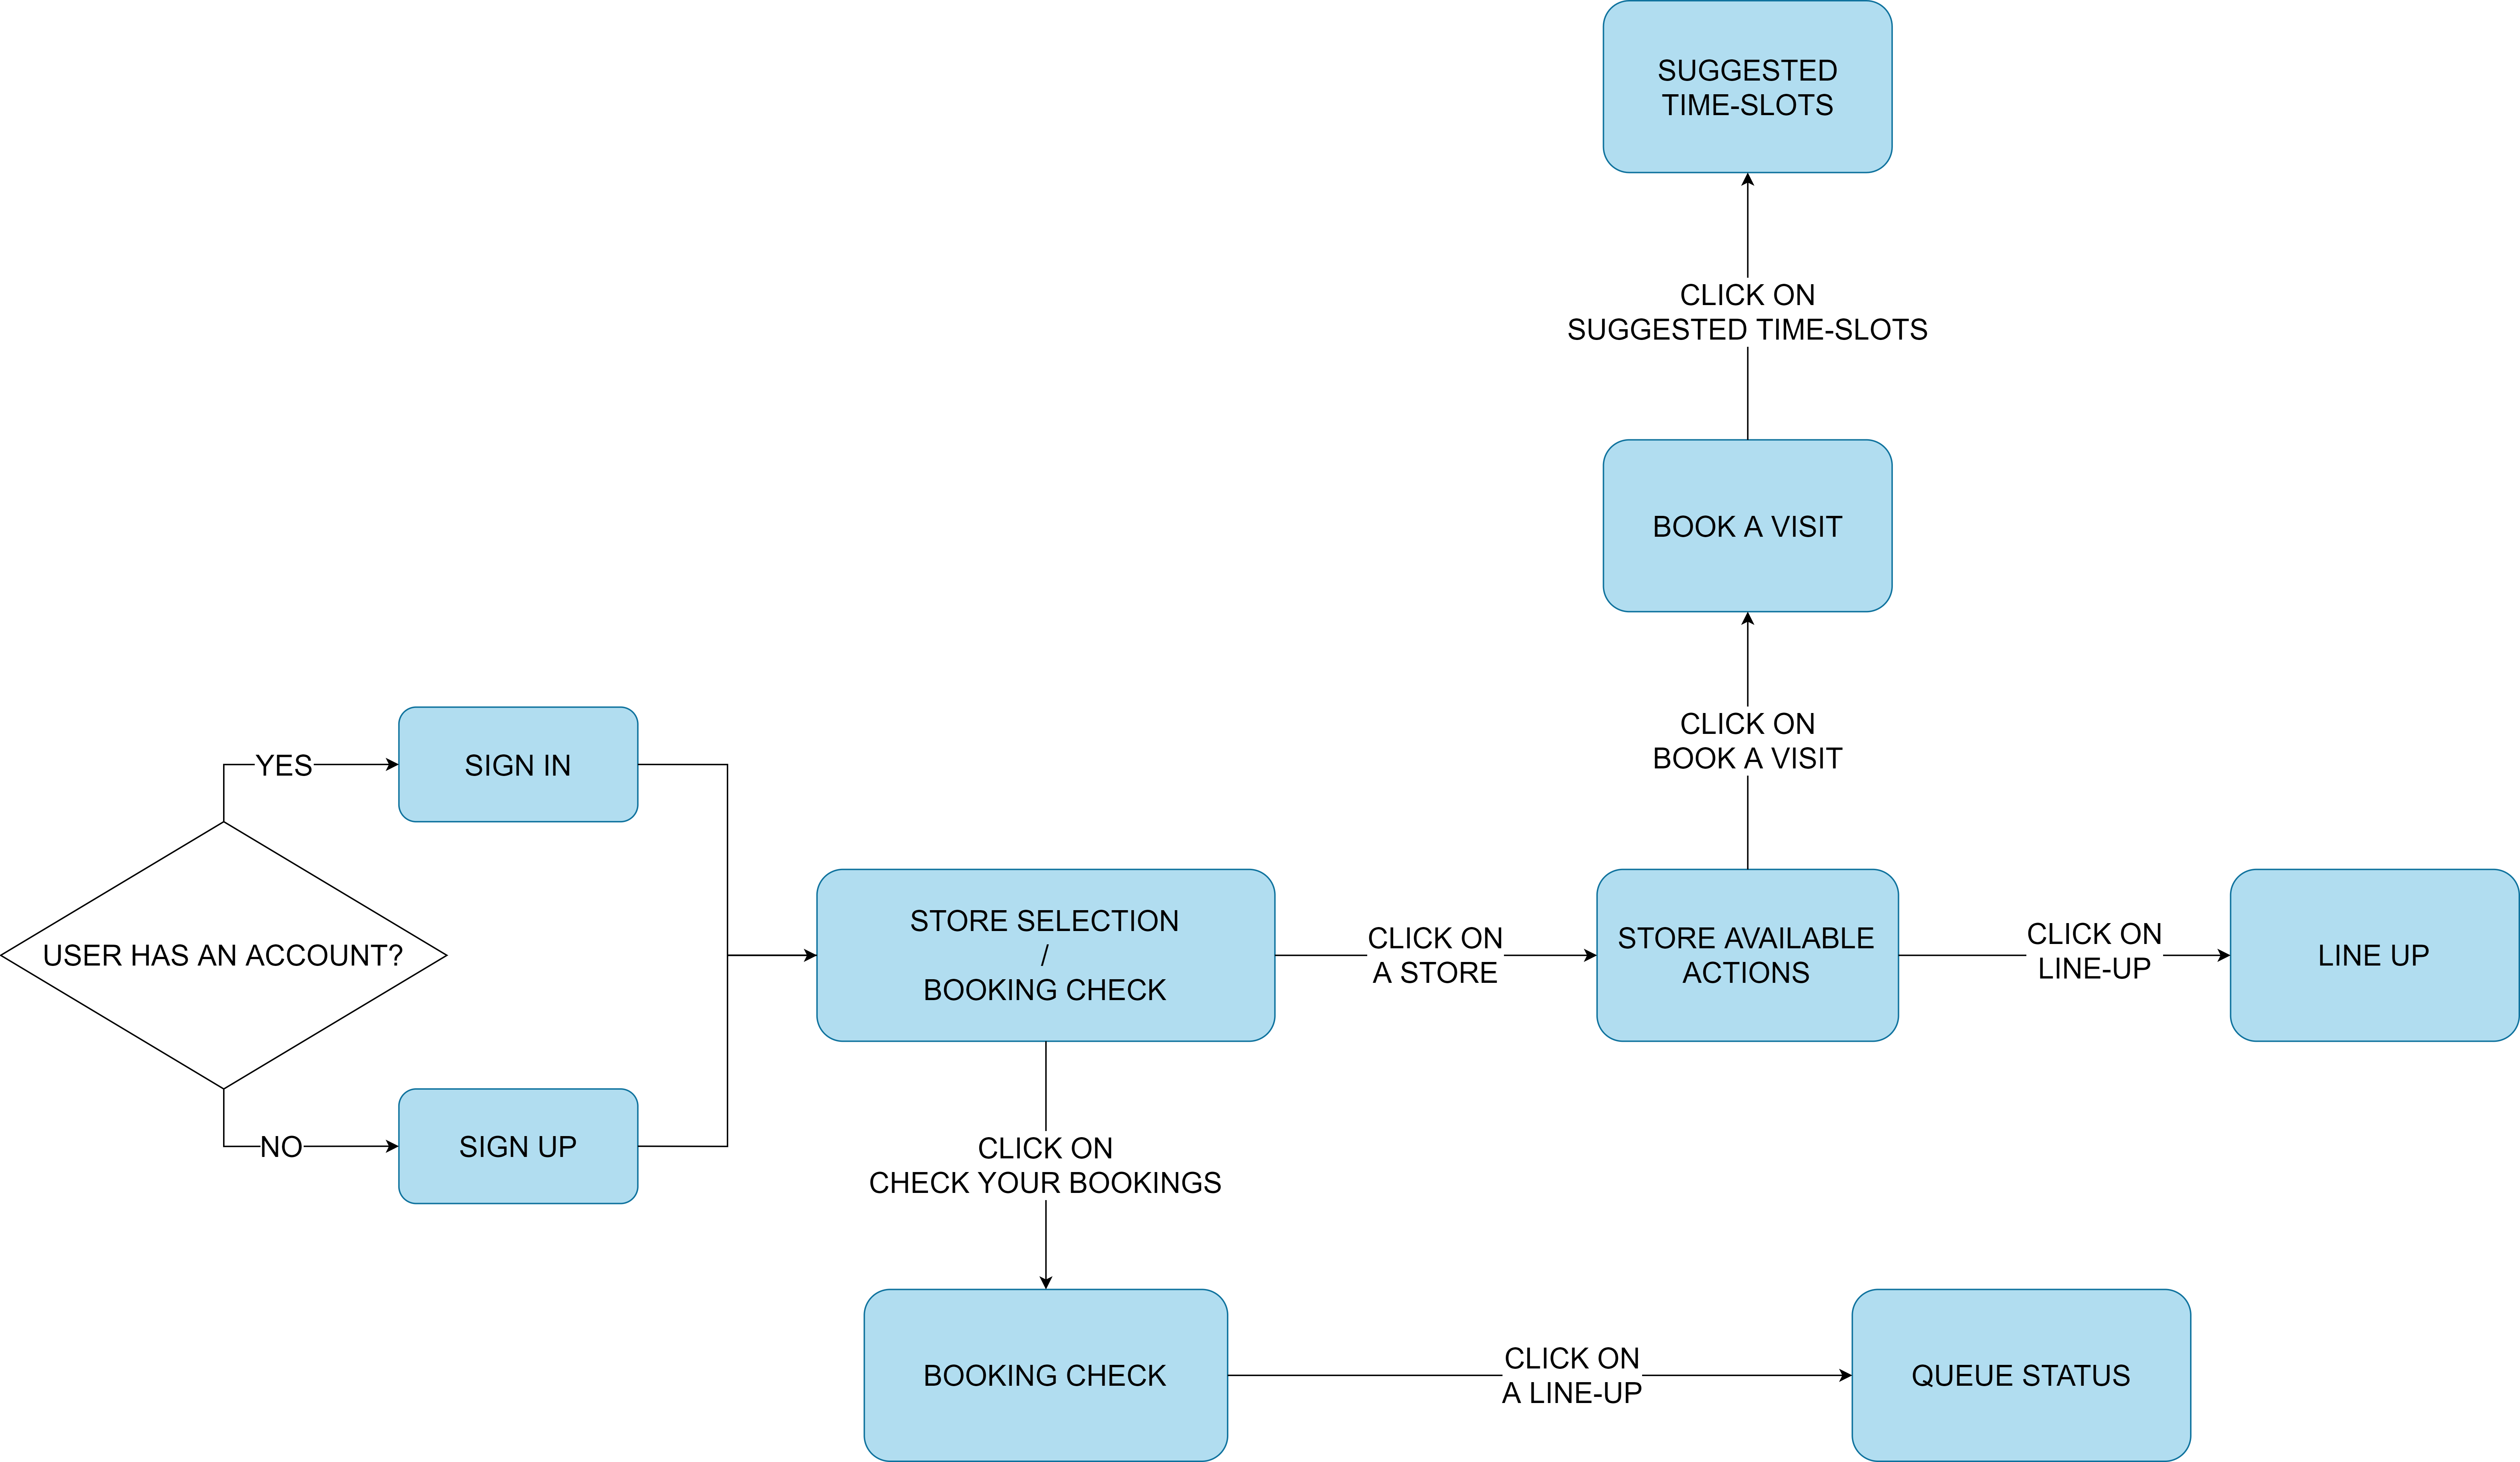
\includegraphics[scale=0.38]{UX diagrams/mobileApp}
			\caption{Mobile App UX diagram}
			\label{fig:MobileAppUXdiagram}
		\end{figure}
		\bigskip \bigskip \bigskip \bigskip
		\begin{figure}[H]
			\centering
			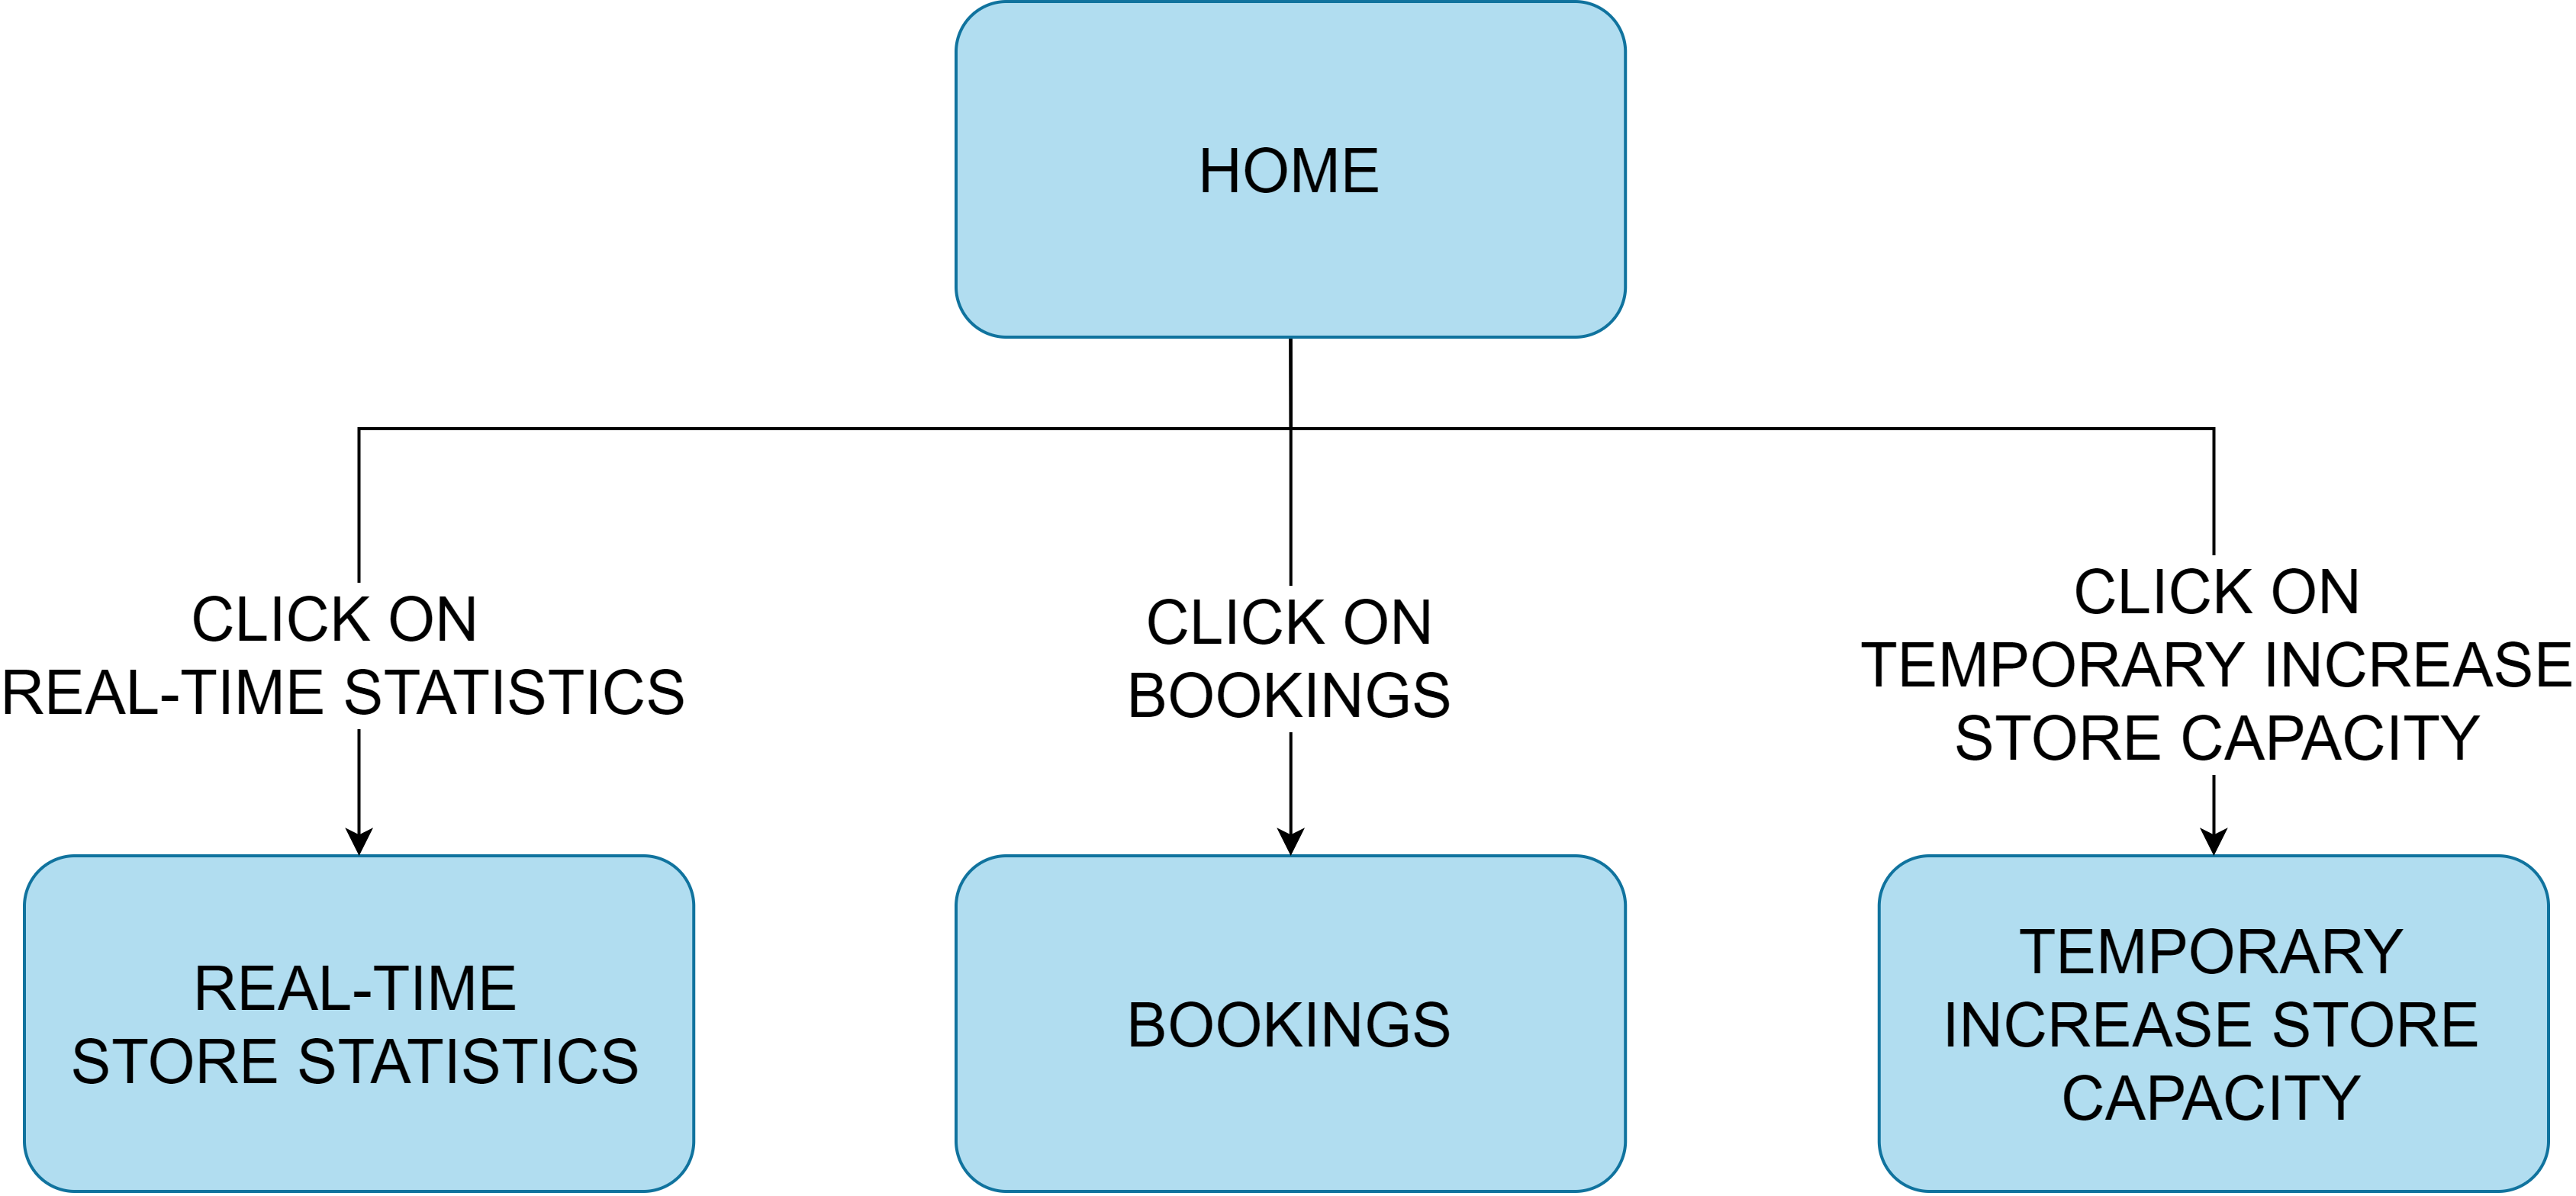
\includegraphics[scale=0.38]{UX diagrams/webAppHome}
			\caption{WebApp UX diagram}
			\label{fig:MobileAppUXdiagram}
		\end{figure}
			
		\newpage
		
			\section{Requirements Traceability}
		
		In this section is presented a mapping between the CLup requirements (the reader can find them in the RASD - section 3.2.1) and the software components - section 2.2. The mapping is made looking for the components that perform the main operations in the satisfaction of a specific requirements. For example, when a costumer line-up in a store a lot of components are involved but the fundamental one, that manages the line-up, is the QueueHandler.
		\bigskip  
		\newline
		\begin{tabular}{|c|l|}
			\hline
			\textbf{REQUIREMENT} & \textbf{MAPPED COMPONENTS} \\ \hline
			R1 & AccessCostumer \\ \hline
			R2 & CostumerMobileApp \\ \hline
			R3 & 
			\begin{minipage}[t]{10cm}
				VisitHandler\\\\
				CostumerHandler\\ 
			\end{minipage} \\ \hline
			R4 & 
			\begin{minipage}[t]{10cm}
				VisitHandler\\\\
				SuggestionsHandler\\\\
				TimetableHandler\\ 
			\end{minipage} \\ \hline
			R5 & QueueHandler \\ \hline
			R6 & 
			\begin{minipage}[t]{10cm}
				VisitHandler\\\\
				SuggestionsHandler\\ 
			\end{minipage} \\ \hline
			R7 & 
			\begin{minipage}[t]{10cm}
				TicketManager\\\\
				QRcodeManager\\ 
			\end{minipage} \\ \hline
			R8 & 
			\begin{minipage}[t]{10cm}
				NotificationsService\\\\
				QueueHandler\\ 
			\end{minipage} \\ \hline
			R9 & NotificationService \\ \hline
			R10 & 
			\begin{minipage}[t]{10cm}
				StatisticsHandler\\\\
				SuggestionsHandler\\ 
			\end{minipage} \\ \hline
			R11 & StatisticsHandler\\ \hline
			R12 & 
			\begin{minipage}[t]{10cm}
				QueueHandler\\\\
				TicketManager\\\\
				QRcodeManager\\ 
			\end{minipage} \\ \hline
		\end{tabular}
		
		\newpage
		\noindent
		\begin{tabular}{|c|l|}
			\hline
			\textbf{REQUIREMENT} & \textbf{MAPPED COMPONENTS} \\ \hline
			R13 & 
			\begin{minipage}[t]{10cm}
				QueueHandler\\\\
				TicketManager\\ 
			\end{minipage} \\ \hline
			R14 & 
			\begin{minipage}[t]{10cm}
				QueueHandler\\\\
				TicketManager\\ 
			\end{minipage} \\ \hline
			R15 & 
			\begin{minipage}[t]{10cm}
				CostumerMobileApp\\\\
				CostumerHandler\\ 
			\end{minipage} \\ \hline
			R16 & 
			\begin{minipage}[t]{10cm}
				VisitHandler\\\\
				StatisticsHandler\\\\
				TimetableHandler\\ 
			\end{minipage} \\ \hline
			R17 & CostumerHandler \\ \hline
			R18 & QueueHandler \\ \hline
			R19 & CostumerHandler \\ \hline
			R20 & 
			\begin{minipage}[t]{10cm}
				VisitHandler\\\\
				StatisticsHandler\\ 
			\end{minipage} \\ \hline
			R21 & 
			\begin{minipage}[t]{10cm}
				QueueHandler\\\\
				TicketManager\\ 
			\end{minipage} \\ \hline
			R22 & StoreHandler \\ \hline						R23 & StoreHandler \\ \hline
			R24 & 
			\begin{minipage}[t]{10cm}
				VisitHandler\\\\
				TimetableHandler\\ 
			\end{minipage} \\ \hline
		\end{tabular}
		
		
		\newpage
		
		\section{Implementation, Integration and Test Plan}
			 \bigskip
			 
			 \subsection{Overview}
			 \medskip
			 Testing is an important practice to make sure that the system behaves as we expect and is able to fulfill the requirements and reach the goals that it is supposed to do. For this reason, the system should be divided in more than a unique block when it is implemented: testing the whole system only when its design has been finished is definitely not a good practice and will lead with every probability to high costs of repair. \\The various components of the system need to be checked independently and then gradually integrated one with the other, with other tests that are subsequent to their integration to make sure that the behavior is exactly what it is expected to be. Of course, it is impossible to find all the bugs in our system through testing, as we know that program testing can be used to show their presence, but not their absence. \\This is the reason why this part of verification and validation is very important: release an application that is as much bug-free as possible. It is important that the verification and validation phases start as soon as the development of the system begins in order to find errors as quickly as possible.\newline\newline
			
			\subsection{Implementation Plan}
			\medskip
			As a consequence of what has been said above and also taking into account that the CLup system is a relatively small one, then it needs to be implemented, tested and integrated following a bottom-up approach. As in unit testing, drivers must be constructed for each leaf module and then, as the system is built up, they will be replaced by higher level components that could use the lower level subsystems’ functionalities. Following this approach, it will be possible to parallelize implementation and the testing procedures.\newline
\noindent
The external components can be assumed to be already reliable, as they are implemented and used without any specific improvements. So, this assumption can be valid for the GoogleMapsService, the StoreSlidingDoors and QRcodeManager components. The integration with the subsystems that interface with them has to be accurately tested and validated.\newline
\noindent
The other components and subsystems that should be considered are the same ones that have been described and shown in the Component View section, that are listed below for the sake of reading them more confortably (the last three ones belong to the client side of the system):
				\begin{itemize}
					\item DBMS Services
					\item Data Manager subsystem
					\item Access Manager subsystem
					\item Store Handler
					\item Customer Handler
					\item Visit subsystem
					\item Queue subsystem
					\item Router
					\item CustomerMobileApp
					\item StoreManagerApp
					\item Ticket Totem
				\end{itemize}
\noindent
The first components that have to be considered are the DBMSServices, because they are the ones that allow to keep system’s data updated to the last version and they allow to write on the Database, always recalling to make it persistent.\\ \newline
The procedure then deals with the Data Manager subsystem, that directly interfaces from the application server towards the DBMS Services and allows to ask and retrieve data through appropriate queries, or to send new data of new info collected during the users’ registrations or their submitted preferences.
Once the Data Manager has been completed, then the other subsystems can be built: Access Manager is independent from the other components, so it can be developed in parallel with other tasks. Because of its purpose, the only role that he has is to guarantee that accesses to the system are authenticated, and this function is perfectly isolated from the others.\\ \newline
In fact, when a customer wants to line up, he has only to face and interact with the Visit and Queue subsystems. Data that are necessary for the bookings and for queuing are retrieved from the Data Manager that takes them from the DB, and then inside the components are elaborated and proposed to the users. The two subsystems – Visit and Queue – do not interact with each other because as the more independent they are, the easier would be in the future to repair and modify them without having to handle other components as a cascade unwanted effect. The only exception is made when the Visit subsystem directly interfaces with the Queue subsystem to update the store’s queue with the addition of a new customer.\\ \newline
Then comes the turn of the Customer Handler and Store Handler components. As the functionalities to store data of a visit have been already implemented and they should properly work, now all the other type of queries of the customers and the store managers can be managed and processed (e.g. booked visits, real time statistics, temporarily increasing the store capacity, …), as their information can be already be stored in the DB.\\ \newline
The Router is the last component that is implemented and tested: its only role is to dispatch messages coming from different parts of the system and assures that they arrive to the right subsystem or component. It has only one main function, but it is very important for the correct behavior of the whole application.
From the point of view of the client components, they can be implemented in parallel to the application server and once the AS has been completely tested, then the two parts can be merged to see if the whole system complies with the requirements and the overall goals.\\ \newline
Finally, we can list what is the strict sequence of constraint of component implementation that must be fulfilled (the client side components and the Access Manager are not included in the following list because their implementation, as previously said, can be done in parallel with the others): 
				\begin{itemize}
					\item DBMS Service
					\item DataManager
					\item Queue subsystem
					\item Visit subsystem
					\item CustomerHandler and StoreHandler
					\item Router
				\end{itemize} 
				\textbf{} \newpage	
				
				
				\subsection{Integration Strategy}
				\medskip
As previously said in the chapter above, the system needs to be implemented with a \textbf{bottom-up approach}. In the following lines there will be a better explanation of how to deal with this procedure, with the different components that will be progressively integrated once they’ve been tested. Drivers are added on the top of the tree-components building because in this way different requests to apply some functions can be done.
\noindent
The first components that have to be unit tested with the DBMSServices are the ones of the Data Manager subsystem. They are the first one that have to be implemented because storing and retrieving data from the DBMS is fundamental for every functionality of the system, that always deals with the most updated state of the system. 
				\begin{figure}[H]
					\centering
					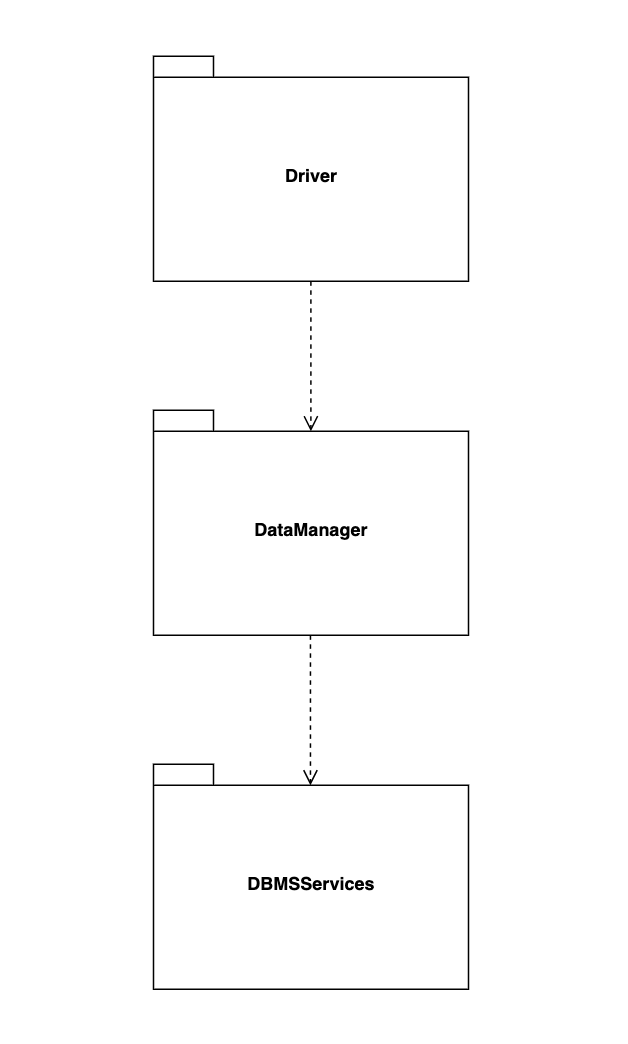
\includegraphics[scale=0.7]{Testing/Testing1.png}
					\caption{}
					\label{fig:Testing}
				\end{figure}
			\newpage
\noindent
It is then the turn of the other components. The Access Manager subsystem can be tested linking it to the Data Manager and testing its functionalities in parallel with the other components that will be explained below. This can happen because it has no direct interaction with the other components.
				\begin{figure}[H]
					\centering
					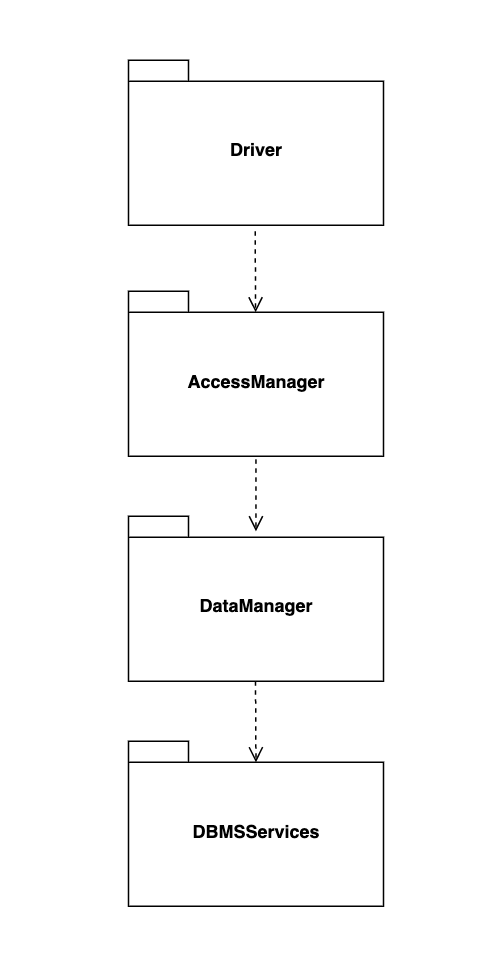
\includegraphics[scale=0.7]{Testing/Testing2.png}
					\caption{}
					\label{fig:Testing}
				\end{figure}
			
		\newpage
\noindent
The external components to which the application server interfaces are supposed to be already tested and validated by their production companies, so the Queue subsystem and its components are the next candidates to be taken into consideration for the unit testing. The testers have to make sure that they can correctly interface to the external components too.
				\begin{figure}[H]
					\centering
					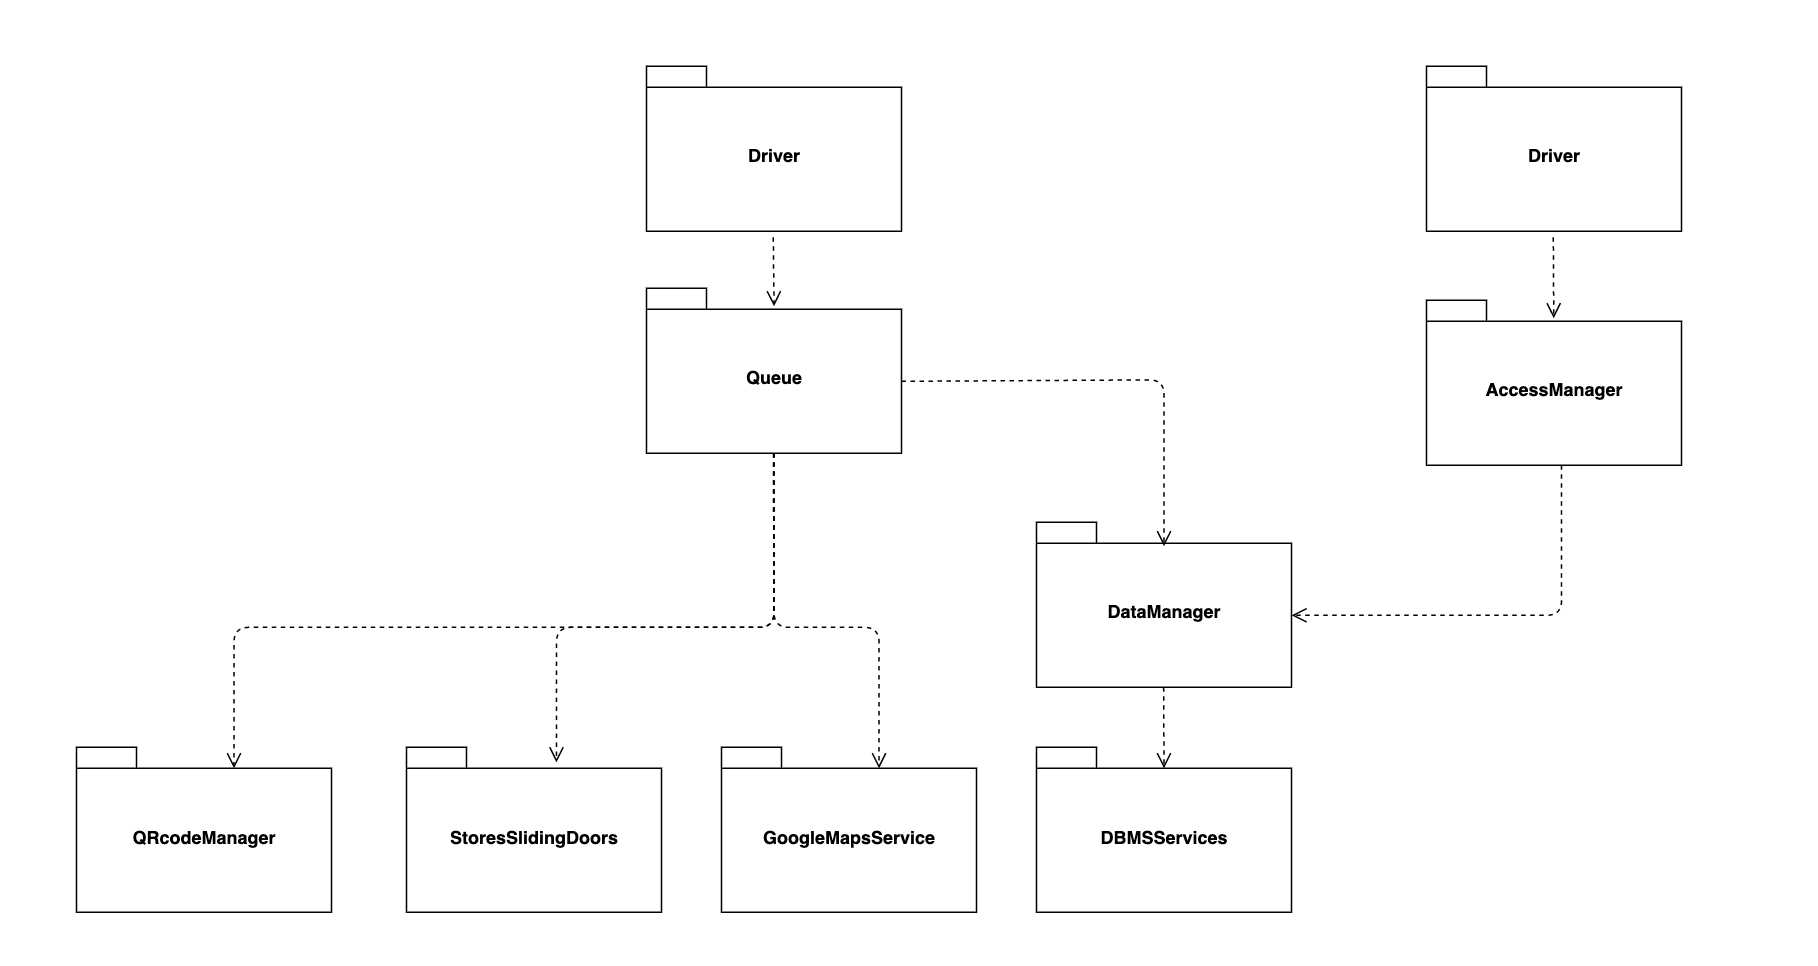
\includegraphics[scale=0.55]{Testing/Testing3.png}
					\caption{}
					\label{fig:Testing}
				\end{figure}
\noindent
When the Queue subsystem has been determined successfully working, the Visit subsystem is the next one to be treated, as it is directly connected with the previously mentioned one. These tests need to be accurately checked as the lining up of a user and his booking procedure have to be as bug-free as possible to guarantee a proper navigation experience.
				\begin{figure}[H]
					\centering
					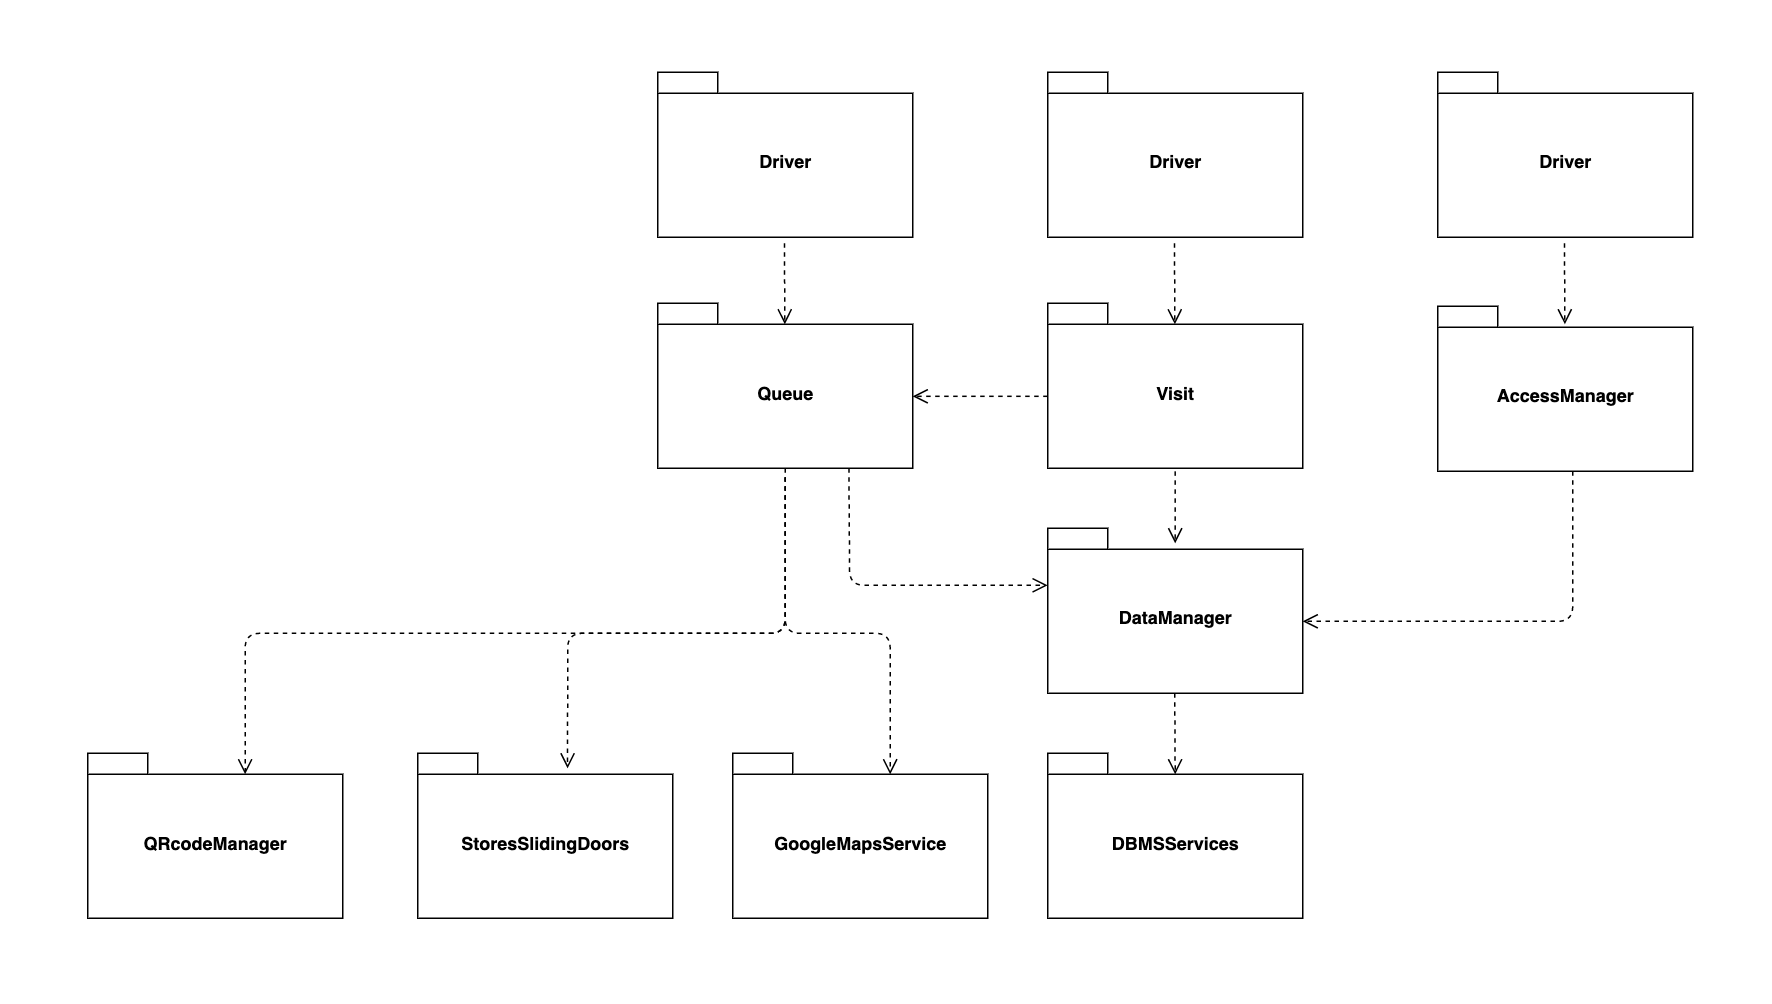
\includegraphics[scale=0.5]{Testing/Testing4.png}
					\caption{}
					\label{fig:Testing}
				\end{figure}
\noindent
Once that these integrations are made, both the Customer Handler and Store Handler components can be unit tested and integrated. Notice that also here the integration with the GoogleMaps Service needs to be made, as the external component is assumed to be perfectly working as we were doing in the previous step. Drivers are properly added to make sure that the step by step integration can be made without any problem, fulfilling all the possible functionalities that a component needs to be ready to deal with.
				\begin{figure}[H]
					\centering
					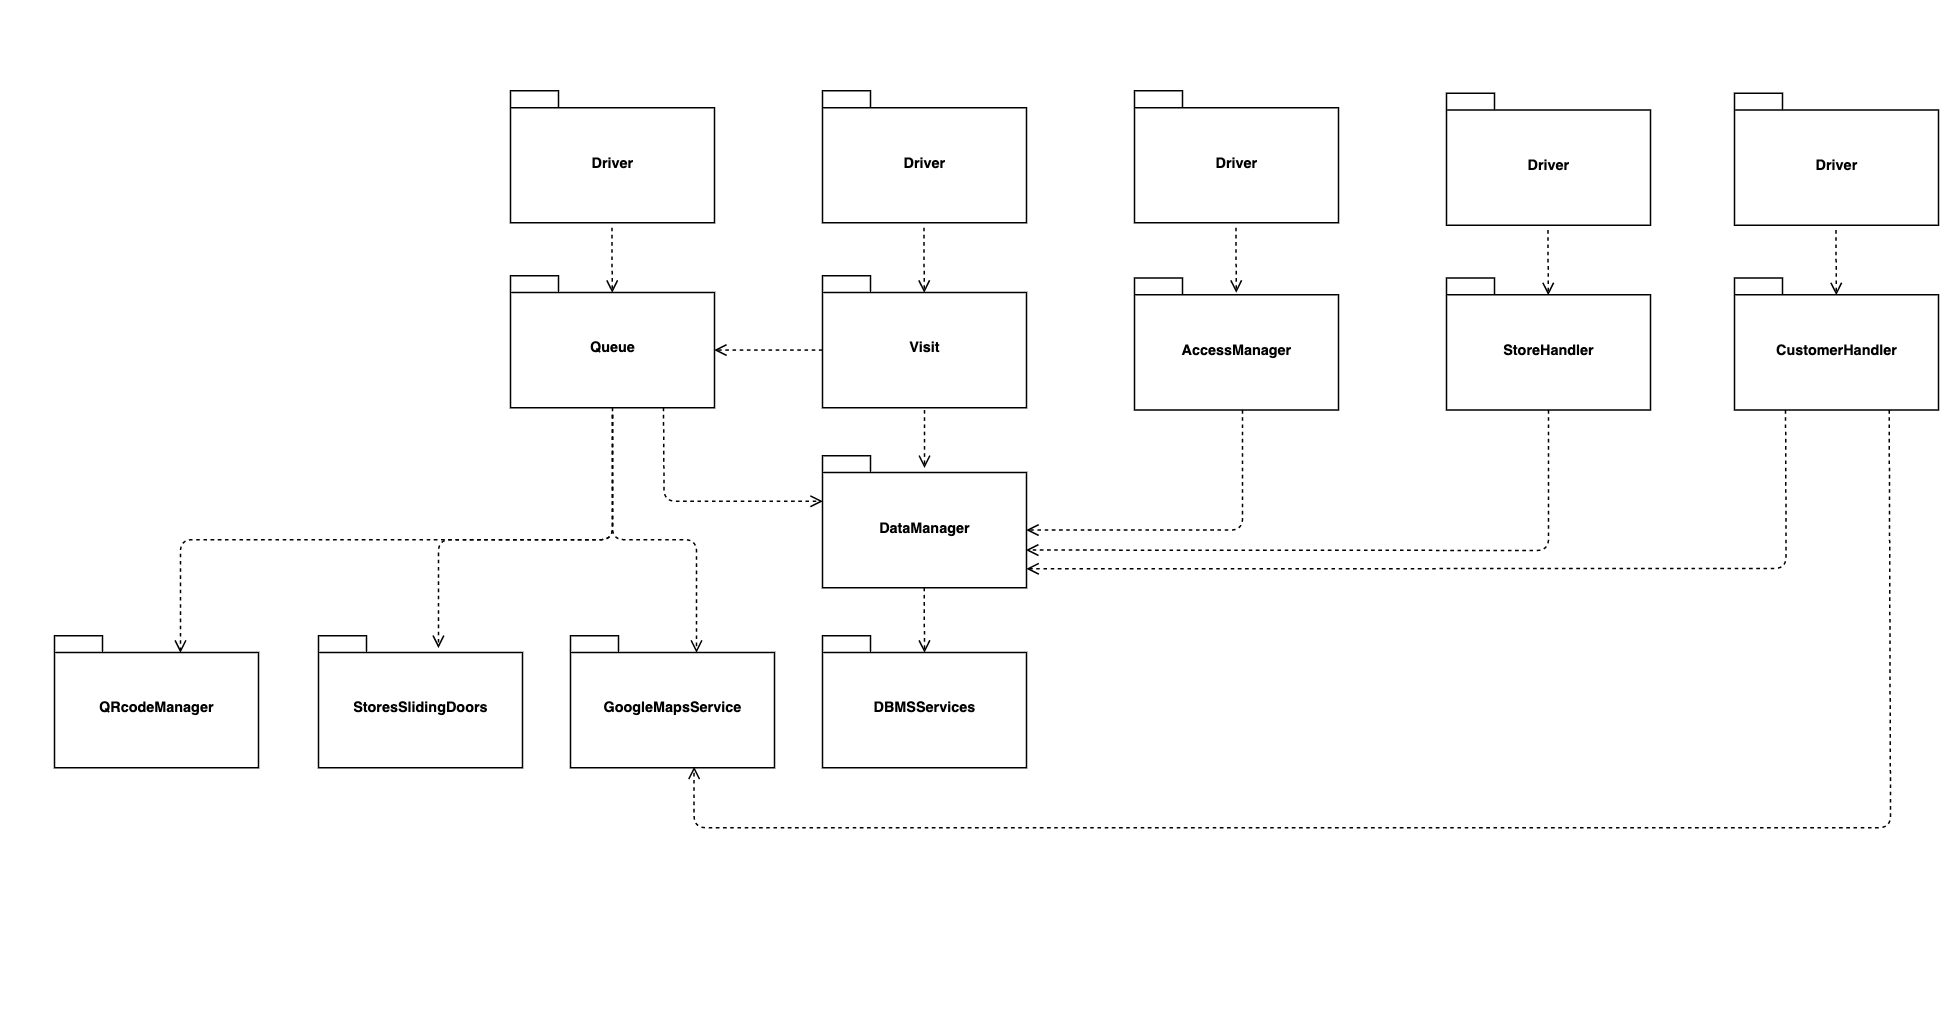
\includegraphics[scale=0.48]{Testing/Testing5.png}
					\caption{}
					\label{fig:Testing}
				\end{figure}
\noindent
To complete the Application Manager the last component that has to be implemented, unit-tested and then added is the Router, that substitutes all the drivers that were drawn in the previous diagram. It allows to make possible the flow of the called methods from the client to the server and dispatch them to the right component.
				\begin{figure}[H]
					\centering
					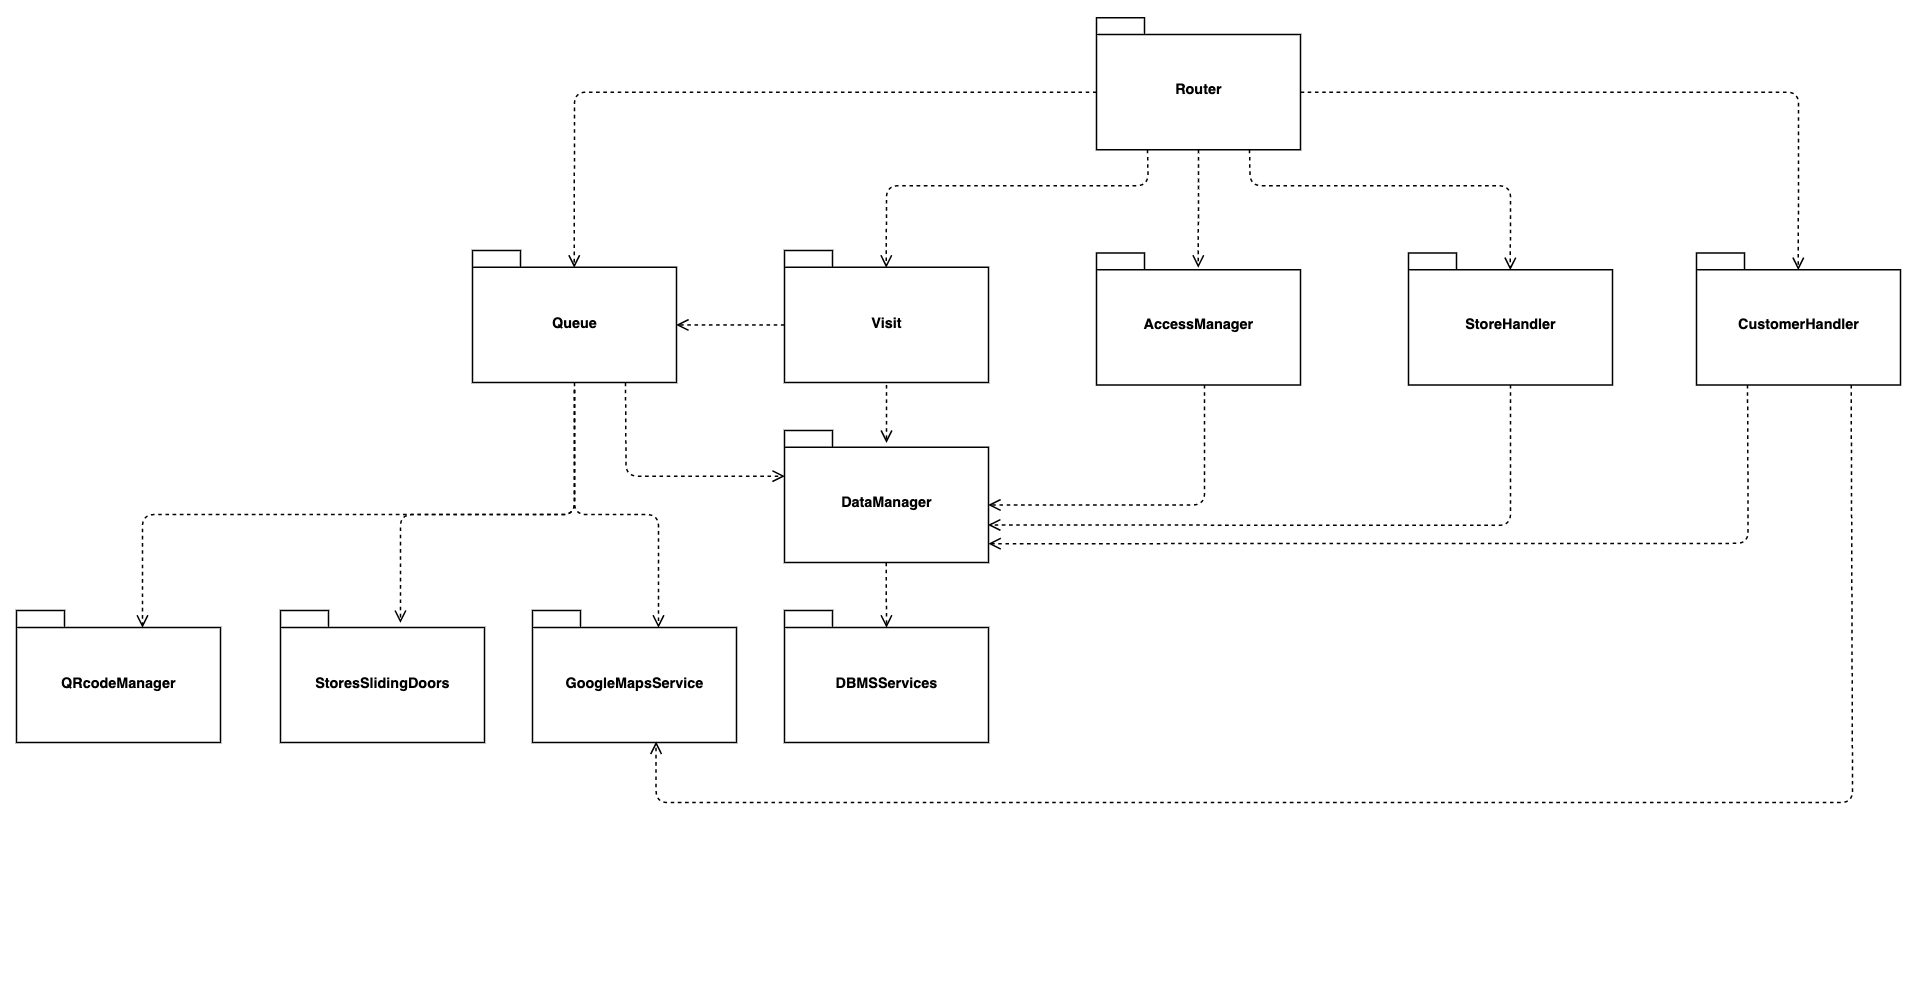
\includegraphics[scale=0.48]{Testing/Testing6.png}
					\caption{}
					\label{fig:Testing}
				\end{figure}
			\newpage
\noindent
In conclusion, Client side components, which can be implemented in parallel to the application server ones, are unit tested and integrated to the whole application system. 
In this way, a final testing session can be performed to validate the overall system.
				\begin{figure}[H]
					\centering
					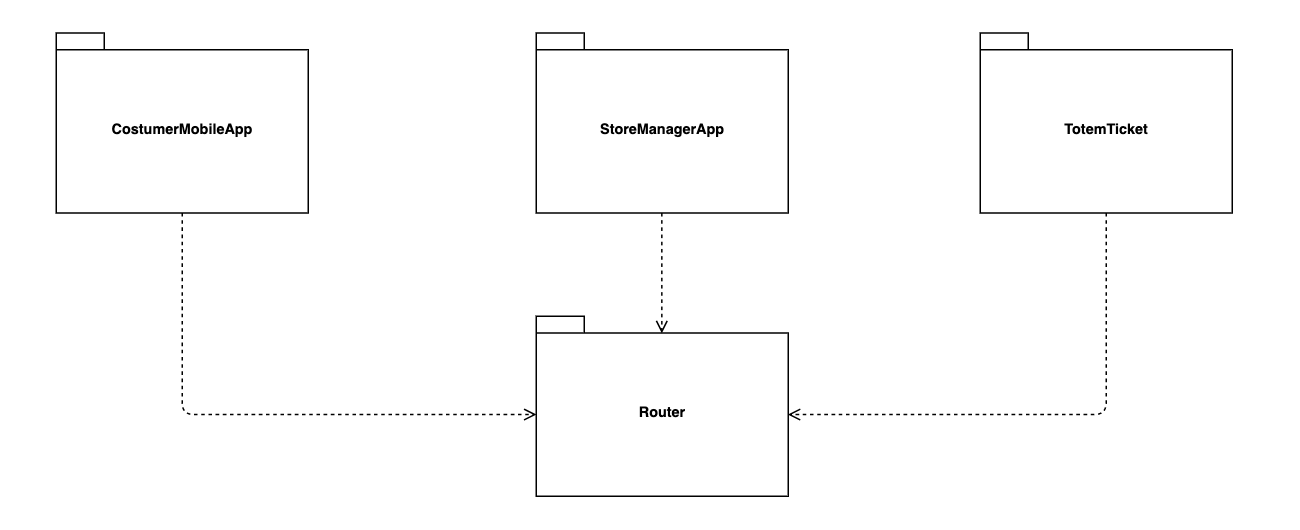
\includegraphics[scale=0.7]{Testing/Testing7.png}
					\caption{}
					\label{fig:Testing}
				\end{figure}


				\subsection{System Testing}
				\medskip
As the integration of the various components of the system has been managed, the whole system testing concerns the check of functional and non-functional requirements, where the testing environment should be as close as possible to the production environment.\\
\textbf{Functional testing}, as the name suggests, verifies the satisfaction of the functional requirements of the system. It’s a good indicator for the correct implementation of the system.\\
Moreover, the \textbf{Load testing}  and \textbf{Performance testing} have a main role in this system: memory leaks, mismanagement of memory and the identification of the upper limits of the components can be made by increasing the load of the system for a long period; what’s more, identifying bottlenecks affecting response time, utilization and throughput makes possible to find inefficient algorithms, optimize queries and if there are any hardware/network issues.\\
\textbf{Stress testing} allows to assure that the system recovers correctly after failure.\\ \newpage



			 
		\section{Effort spent}
			
			\medskip
			\textbf{\large Antonio Ercolani:} \\ \newline
			\begin{tabular}{|l|c|}
				\hline
				\begin{minipage}[t]{10cm}
				Purpose and Document Structure
				\end{minipage} 
				& \textbf{1h} \\ \hline
				\rowcolor[HTML]{DCDCDC} 
				User Interface Design & \textbf{10h} \\ \hline
				Component view discussion & \textbf{3h} \\ \hline
				\rowcolor[HTML]{DCDCDC} 
				Component view & \textbf{3h} \\ \hline
				Deployment view & \textbf{4h} \\ \hline
				\rowcolor[HTML]{DCDCDC} 
				Sequence diagrams & \textbf{6h} \\ \hline
				Requirement traceability table \& discussion & \textbf{2h} \\ \hline
				\rowcolor[HTML]{DCDCDC} 
				Selected architectural styles and patterns  & \textbf{3h} \\ \hline
				Review meetings  & \textbf{7h} \\ \hline
				\rowcolor[HTML]{DCDCDC} 
				Various fixes  & \textbf{3h} \\ \hline
				
			\end{tabular}
			\newline
			\newline
			
			\medskip
			\textbf{\large Vittorio Fabris:} \\ \newline
			\begin{tabular}{|l|c|}
				\hline
				\begin{minipage}[t]{10cm}
					Scope and organization of chapter 1
				\end{minipage} 
				& \textbf{1,5h} \\ \hline
				\rowcolor[HTML]{DCDCDC} 
				 Architectural Design Overview & \textbf{3h} \\ \hline
				 Component view discussion & \textbf{3h} \\ \hline
				\rowcolor[HTML]{DCDCDC} 
				Component View & \textbf{8h} \\ \hline
				Validation and Testing & \textbf{12h} \\ \hline
				\rowcolor[HTML]{DCDCDC} 
				Review meetings & \textbf{7h} \\ \hline
				Various fixes & \textbf{2h} \\ \hline
			\end{tabular}
		\newline \newline
		\newpage
		\medskip
		\textbf{\large Riccardo Nannini:} \\ \newline
		\begin{tabular}{|l|c|}
			\hline
			\begin{minipage}[t]{10cm}
				Component view discussion
			\end{minipage} 
			& \textbf{3h} \\ \hline
			\rowcolor[HTML]{DCDCDC} 
			Component view & \textbf{3h} \\ \hline
			Component interfaces & \textbf{3,5h} \\ \hline
			\rowcolor[HTML]{DCDCDC} 
			UML model & \textbf{2h} \\ \hline
			Runtime view & \textbf{4,5h} \\ \hline
			\rowcolor[HTML]{DCDCDC} 
			Algorithms and data structures & \textbf{4,5h} \\ \hline
			Review meetings & \textbf{7h} \\ \hline
			\rowcolor[HTML]{DCDCDC} 
			Various fixes & \textbf{2,5h} \\ \hline
		\end{tabular}
		\bigskip
			
			\section{References}	
				\begin{itemize}
				\item Mockups were made using \textit{www.justinmind.com}
				\item VCS Git + Hosting with GitHub \textit{github.com}
				\item The diagrams were made using \textit{www.draw.io}
				\item Software Engineering 2 course material - Politecnico di Milano 2020-2021
			\end{itemize}
			
	

				
\end{document}
